\documentclass[10pt]{article}
\usepackage[vietnamese]{babel}
\usepackage[utf8]{inputenc}
\usepackage[T5]{fontenc}
\usepackage{amsmath}
\usepackage{amsfonts}
\usepackage{amssymb}
\usepackage[version=4]{mhchem}
\usepackage{stmaryrd}
\usepackage{graphicx}
\usepackage[export]{adjustbox}
\graphicspath{ {./images/} }
\usepackage{caption}
\usepackage{multirow}

\title{Bài 6. XU HƯÓNG BIẾN ĐỔI MỘT SỐ TÍNH CHẤT CỦA NGUYÊN TƯ CÁC NGUYÊN TỐ TRONG MỘT CHU Kİ VÀ TRONG MỘT NHÓM }

\author{}
\date{}


\begin{document}
\maketitle
\captionsetup{singlelinecheck=false}
\section*{CHUONG 1 CẤU TAO NGUYÊN TỬ}
\section*{Bài 1. THÀNH PHẦN CỦA NGUYÊN TỬ}
\section*{NHẬN BIÉT}
1.1. Phát biểu nào sau đây không đúng?\\
A. Nguyên tử được cấu thành từ các hạt cơ bản là proton, neutron và electron.\\
B. Nguyên tử có cấu trúc đặc khít, gồm vỏ nguyên tử và hạt nhân nguyên tử.\\
C. Hạt nhân nguyên tử cấu thành từ các hạt proton và neutron.\\
D. Vỏ nguyên tử cấu thành từ các hạt electron.\\
1.2. Trường hợp nào sau đây có sự tương ứng giữa hạt cơ bản với khối lượng và điện tích của chúng?\\
A. Proton, $\mathrm{m} \approx 0,00055$ amu, $\mathrm{q}=+1$.\\
B. Neutron, $\mathrm{m} \approx 1 \mathrm{amu}, \mathrm{q}=0$.\\
C. Electron, $\mathrm{m} \approx 1 \mathrm{amu}, \mathrm{q}=-1$.\\
D. Proton, $\mathrm{m} \approx 1 \mathrm{amu}, \mathrm{q}=-1$.\\
1.3. Nếu đường kính của nguyên tử khoảng $10^{2} \mathrm{pm}$ thì đường kính của hạt nhân khoảng\\
A. $10^{2} \mathrm{pm}$.\\
B. $10^{-4} \mathrm{pm}$.\\
C. $10^{-2} \mathrm{pm}$.\\
D. $10^{4} \mathrm{pm}$.\\
1.4. Viết lại bảng sau vào vở và điền thông tin còn thiếu vào các ô trống:

\begin{center}
\begin{tabular}{|c|c|c|c|c|c|c|}
\hline
Nguyên tố & Kí hiệu & Z & Số e & Số $\mathbf{p}$ & Số n & Số khối \\
\hline
Carbon & C & 6 & 6 & $?$ & 6 & $?$ \\
\hline
Nitrogen & N & 7 & $?$ & 7 & $?$ & 14 \\
\hline
Oxygen & O & 8 & 8 & $?$ & 8 & $?$ \\
\hline
Sodium (natri) & Na & 11 & $?$ & 11 & $?$ & 23 \\
\hline
\end{tabular}
\end{center}

\section*{THÔNG HIỂU}
1.5. Bằng cách nào có thể tạo ra chùm electron? Nêu khối lượng và điện tích của electron.\\
1.6. Fluorine và hợp chất của nó được sử dụng làm chất chống sâu răng, chất cách điện, chất làm lạnh, vật liệu chống dính,... Nguyên tử fluorine chứa 9 electron và có số khối là 19. Tổng số hạt proton, electron và neutron trong nguyên tử fluorine là\\
A. 19 .\\
B. 28 .\\
C. 30 .\\
D. 32 .\\
1.7. Khối lượng của nguyên tử magnesium là $39,8271 \cdot 10^{-27} \mathrm{~kg}$. Khối lượng của magnesium theo amu là\\
A. 23,978 .\\
B. $66,133 \cdot 10^{-51}$.\\
C. 24,000 .\\
D. $23,985 \cdot 10^{-3}$.\\
1.8. Khối lượng tuyệt đối của một nguyên tử oxygen bằng $26,5595 \cdot 10^{-27} \mathrm{~kg}$. Hãy tính khối lượng nguyên tử (theo amu) và khối lượng mol nguyên tử (theo g ) của nguyên tử này.

\section*{VẬN DỤNG}
1.9. Tổng số các hạt proton, neutron và electron trong nguyên tử của nguyên tố X là 10 . Số khối của nguyên tử nguyên tố X là\\
A. 3 .\\
B. 4 .\\
C. 6 .\\
D. 7 .\\
1.10. Nguyên tử helium có 2 proton, 2 neutron và 2 electron. Khối lượng của các electron chiếm bao nhiêu \% khôi lượng nguyên tử helium?\\
A. $2,72 \%$.\\
B. $0,272 \%$.\\
C. $0,0272 \%$.\\
D. $0,0227 \%$.\\
1.11. Hợp kim chứa nguyên tố X nhẹ và bền, dùng chế tạo vỏ máy bay, tên lửa. Nguyên tố X còn được sử dụng trong xây dựng, ngành điện và đồ gia dụng. Nguyên tử của nguyên tố X có tổng số hạt (proton, electron, neutron) là 40 . Tổng số hạt mang điện nhiều hơn tổng số hạt không mang điện là 12 .\\
a) Tính số mỗi loại hạt (proton, electron, neutron) trong nguyên tử X .\\
b) Tính số khối của nguyên tử X .\\
1.12. Nguyên tử aluminium (nhôm) gồm 13 proton và 14 neutron. Tính khối lượng proton, neutron, electron có trong 27 g nhôm.\\
1.13. Xác định khối lượng của hạt nhân nguyên tử boron chứa 5 proton, 6 neutron và khối lượng nguyên tử boron. So sánh hai kết quả tính được và nêu nhận xét.

\section*{Bài 2. NGUYÊN TỐ HOÁ HỌC}
\section*{NHẬN BIẾT}
2.1. Phát biểu nào sau đây không đúng?\\
A. Số hiệu nguyên tử bằng số đơn vị điện tích hạt nhân nguyên tử.\\
B. Số khối của hạt nhân bằng tổng số proton và số neutron.\\
C. Trong nguyên tử, số đơn vị điện tích hạt nhân bằng số proton và bằng số neutron.\\
D. Nguyên tố hoá học là những nguyên tử có cùng số đơn vị điện tích hạt nhân.\\
2.2. Số hiệu nguyên tử cho biết thông tin nào sau đây?\\
A. Số proton.\\
B. Số neutron.\\
C. Số khối.\\
D. Nguyên tử khối.\\
2.3. Dãy nào sau đây gồm các đồng vị của cùng một nguyên tố hoá học?\\
A. ${ }_{6}^{14} \mathrm{X},{ }_{7}^{14} \mathrm{Y},{ }_{8}^{14} \mathrm{Z}$.\\
B. ${ }_{9}^{19} \mathrm{X},{ }_{10}^{19} \mathrm{Y},{ }_{10}^{20} \mathrm{Z}$.\\
C. ${ }_{14}^{28} \mathrm{X},{ }_{14}^{29} \mathrm{Y},{ }_{14}^{30} \mathrm{Z}$.\\
D. ${ }_{18}^{40} X,{ }_{19}^{40} Y,{ }_{20}^{40} Z$.\\
2.4. Kí hiệu nguyên tử nào sau đây viết đúng?\\
A. ${ }_{7}^{15} \mathrm{~N}$.\\
B. ${ }^{16} \mathrm{O}$.\\
C. 16 S .\\
D. $\mathrm{Mg}_{12}^{24}$.\\
2.5. Thông tin nào sau đây không đúng về ${ }_{82}^{206} \mathrm{~Pb}$ ?\\
A. Số đơn vị điện tích hạt nhân là 82 .\\
B. Số proton và neutron là 82 .\\
C. Số neutron là 124 .\\
D. Số khối là 206 .

\section*{THÔNG HIỂU}
2.6. Cho kí hiệu các nguyên tử sau:

$$
{ }_{6}^{14} \mathrm{X},{ }_{7}^{14} \mathrm{Y},{ }_{8}^{16} \mathrm{Z},{ }_{9}^{19} \mathrm{~T},{ }_{8}^{17} \mathrm{Q},{ }_{9}^{16} \mathrm{M},{ }_{10}^{19} \mathrm{E},{ }_{7}^{16} \mathrm{G},{ }_{8}^{18} \mathrm{~L} .
$$

Dãy nào sau đây gồm các nguyên tử thuộc cùng một nguyên tố hoá học?\\
A. ${ }_{6}^{14} \mathrm{X},{ }_{7}^{14} \mathrm{Y},{ }_{8}^{16} \mathrm{Z}$.\\
B. ${ }_{8}^{16} \mathrm{Z},{ }_{9}^{16} \mathrm{M},{ }_{7}^{16} \mathrm{G}$.\\
C. ${ }_{8}^{17} \mathrm{Q},{ }_{9}^{16} \mathrm{M},{ }_{10}^{19} \mathrm{E}$.\\
D. ${ }_{8}^{16} \mathrm{Z},{ }_{8}^{17} \mathrm{Q},{ }_{8}^{18} \mathrm{~L}$.\\
2.7. Nitrogen có hai đồng vị bền là ${ }_{7}^{14} \mathrm{~N}$ và ${ }_{7}^{15} \mathrm{~N}$. Oxygen có ba đồng vị bền là ${ }_{8}^{16} \mathrm{O},{ }_{8}^{17} \mathrm{O}$ và ${ }_{8}^{18} \mathrm{O}$. Số hợp chất $\mathrm{NO}_{2}$ tạo bởi các đồng vị trên là\\
A. 3 .\\
B. 6 .\\
C. 9.\\
D. 12 .\\
2.8. Trong tự nhiên, bromine có hai đồng vị bền là ${ }_{35}^{79} \mathrm{Br}$ chiếm $50,69 \%$ số nguyên tử và ${ }_{35}^{81} \mathrm{Br}$ chiếm $49,31 \%$ số nguyên tử. Nguyên tử khối trung bình của bromine là\\
A. 80,00 .\\
B. 80,112 .\\
C. 80,986 .\\
D. 79,986 .\\
2.9. Oxygen có ba đồng vị với tỉ lệ \% số nguyên tử tương ứng là ${ }^{16} \mathrm{O}(99,757 \%)$, ${ }^{17} \mathrm{O}(0,038 \%),{ }^{18} \mathrm{O}(0,205 \%)$. Nguyên tử khối trung bình của oxygen là\\
A. 16,0 .\\
B. 16,2 .\\
C. 17,0 .\\
D. 18,0 .

\section*{VẬN DỤNG}
2.10. Nguyên tố $R$ có hai đồng vị, nguyên tử khối trung bình là 79,91 . Một trong hai đồng vị là ${ }^{79} \mathrm{R}$ (chiếm $54,5 \%$ ). Nguyên tử khối của đồng vị thứ hai là\\
A. 80 .\\
B. 81 .\\
C. 82.\\
D. 80,5 .\\
2.11. Boron là nguyên tố có nhiều tác dụng đối với cơ thể người như: làm lành vết thương, điều hoà nội tiết sinh dục, chống viêm khớp,... Do ngọn lửa cháy có màu lục đặc biệt nên boron vô định hình được dùng làm pháo hoa. Boron có hai đồng vị là ${ }^{10} \mathrm{~B}$ và ${ }^{11} \mathrm{~B}$, nguyên tử khối trung bình là 10,81 . Tính phần trăm số nguyên tử mỗi đồng vị của boron.\\
2.12. Đồng vị phóng xạ cobalt (Co-60) phát ra tia $\gamma$ có khả năng đâm xuyên mạnh, dùng điều trị các khối u ở sâu trong cơ thể. Cobalt có ba đồng vị: ${ }_{27}^{59} \mathrm{Co}$ (chiếm $98 \%$ ), ${ }_{27}^{58} \mathrm{Co}$ và ${ }_{27}^{60} \mathrm{Co}$; nguyên tử khối trung bình là 58,982 . Xác định hàm lượng \% của đồng vị phóng xạ Co-60.

\section*{Bài 3. CẤU TRÚC LỚP VỎ ELECTRON NGUYÊN TỬ}
\section*{NHẬN BIẾT}
3.1. Orbital nguyên tử là\\
A. đám mây chứa electron có dạng hình cầu.\\
B. đám mây chứa electron có dạng hình số 8 nổi.\\
C. khu vực không gian xung quanh hạt nhân mà tại đó xác suất có mặt electron lớn nhất.\\
D. quỹ đạo chuyển động của electron quay quanh hạt nhân có kích thước và năng lượng xác định.\\
3.2. Sự phân bố electron trong một orbital dựa vào nguyên lí hay quy tắc nào sau đây?\\
A. Nguyên lí vững bền.\\
B. Quy tắc Hund.\\
C. Nguyên lí Pauli.\\
D. Quy tắc Pauli.\\
3.3. Sự phân bố electron trên các phân lớp thuộc các lớp electron dựa vào nguyên lí hay quy tắc nào sau đây?\\
A. Nguyên lí vững bền và nguyên lí Pauli.\\
B. Nguyên lí vững bền và quy tắc Hund.\\
C. Nguyên lí Pauli và quy tắc Hund.\\
D. Nguyên lí vững bền và quy tắc Pauli.\\
3.4. Sự phân bố electron vào các lớp và phân lớp căn cứ vào\\
A. nguyên tử khối tăng dần.\\
B. điện tích hạt nhân tăng dần.\\
C. số khối tăng dần.\\
D. mức năng lượng electron.\\
3.5. Ở trạng thái cơ bản, trong nguyên tử, electron chiểm các mức năng lượng\\
A. lần lượt từ cao đến thấp.\\
B. lần lượt từ thấp đến cao.\\
C. bất kì.\\
D. từ mức thứ hai trở đi.\\
3.6. Các lớp electron được đánh số từ trong ra ngoài bằng các số nguyên dương: $\mathrm{n}=1,2,3, \ldots$ với tên gọi là các chữ cái in hoa là\\
A. $\mathrm{K}, \mathrm{L}, \mathrm{M}, \mathrm{O}, \ldots$\\
B. $L, M, N, O, \ldots$\\
C. $\mathrm{K}, \mathrm{L}, \mathrm{M}, \mathrm{N}, \ldots$\\
D. $\mathrm{K}, \mathrm{M}, \mathrm{N}, \mathrm{O}, \ldots$\\
3.7. Các phân lớp trong mỗi lớp electron được kí hiệu bằng các chữ cái viết thường, theo thứ tự là\\
A. $s, d, p, f, \ldots$\\
B. s, p, d, f,\\
C. s, p, f, d, ...\\
D. $\mathrm{f}, \mathrm{d}, \mathrm{p}, \mathrm{s}, \ldots$\\
3.8. Phát biểu nào sau đây đúng?\\
A. Những electron ở lớp K có mức năng lượng thấp nhất.\\
B. Những electron ở gần hạt nhân có mức năng lượng cao nhất.\\
C. Electron ở orbital 3 p có mức năng lượng thấp hơn electron ở orbital 3 s .\\
D. Các electron trong cùng một lớp có năng lượng bằng nhau.\\
3.9. Mỗi orbital nguyên tử chứa tối đa\\
A. 1 electron.\\
B. 2 electron.\\
C. 3 electron.\\
D. 4 electron.\\
3.10. Số orbital trong các phân lớp $\mathrm{s}, \mathrm{p}, \mathrm{d}$ lần lượt bằng\\
A. $1,3,5$.\\
B. $1,2,4$.\\
C. $3,5,7$.\\
D. $1,2,3$.

\section*{THÔNG HIỂU}
3.11. Phân lớp 3d có số electron tối đa là\\
A. 6 .\\
B. 18 .\\
C. 14.\\
D. 10 .\\
3.12. Lớp L có số phân lớp electron bằng\\
A. 1 .\\
B. 2 .\\
C. 3 .\\
D. 4 .\\
3.13. Lớp M có số orbital tối đa bằng\\
A. 3 .\\
B. 4 .\\
C. 9.\\
D. 18 .\\
3.14. Lớp M có số electron tối đa bằng\\
A. 3 .\\
B. 4 .\\
C. 9.\\
D. 18 .\\
3.15. Các electron của nguyên tử nguyên tố X được phân bố trên ba lớp, lớp thứ ba có 6 electron. Số đơn vị điện tích hạt nhân của nguyên tử nguyên tố X là\\
A. 6 .\\
B. 8 .\\
C. 14.\\
D. 16 .\\
3.16. Nguyên tố X có $\mathrm{Z}=17$. Electron lớp ngoài cùng của nguyên tử nguyên tố X thuộc lớp\\
A. K.\\
B. L.\\
C. M.\\
D. N.\\
3.17. Cách biểu diễn electron trong AO nào sau đây không tuân theo nguyên lí Pauli?\\
A. $\square$ B. $\square$ C. $\square$ D. $\square$\\
$\square$\\
3.18. Sự phân bố electron theo ô orbital nào dưới đây là đúng?\\
A. $\square$ .\\
C.\\
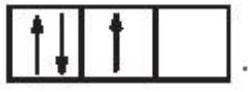
\includegraphics[max width=\textwidth, center]{2025_10_23_daab5c8457c85b365b9eg-06(1)}\\
B.\\
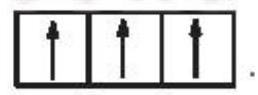
\includegraphics[max width=\textwidth, center]{2025_10_23_daab5c8457c85b365b9eg-06(2)}\\
D.\\
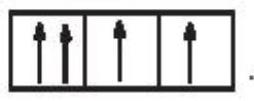
\includegraphics[max width=\textwidth, center]{2025_10_23_daab5c8457c85b365b9eg-06}\\
3.19. Dùng ô orbital để mô tả cách sắp xếp electron trong orbital s .\\
3.20. Trường hợp trong orbital p có chứa hai electron thì có những cách nào biểu diễn electron trong orbital đó? Cách nào tuân theo quy tắc Hund?\\
3.21. Nêu mối quan hệ về năng lượng của electron trên các orbital, các phân lớp, các lớp electron.\\
3.22. Cho biết tổng số electron tối đa chứa trong:\\
a) Phân lớp p ;\\
b) Phân lớp d;\\
c) Lớp K ;\\
d) Lớp M.

\section*{VÂN DỤNG}
3.23. Nguyên tố X có $\mathrm{Z}=12$ và nguyên tố Y có $\mathrm{Z}=17$.

Viết cấu hình electron nguyên tử của nguyên tố X và Y . Khi nguyên tử của nguyên tố X nhường đi hai electron và nguyên tử của nguyên tố Y nhận thêm một electron thì lớp electron ngoài cùng của chúng có đặc điểm gi?\\
3.24. Viết cấu hình electron theo ô orbital của nguyên tử các nguyên tố có $Z=9, Z=14$ và $Z=21$. Chúng là nguyên tố kim loại, phi kim hay khí hiếm?\\
3.25. Hợp chất A có công thức $\mathrm{M}_{4} \mathrm{X}_{3}$. Tổng số hạt proton, electron và neutron trong phân tử A là 214 . Tổng số hạt proton, neutron, electron của $[\mathrm{M}]_{4}$ nhiều hơn so với $[\mathrm{X}]_{3}$ trong A là 106 .\\
a) Xác định công thức hoá học của A .\\
b) Viết cấu hình electron của các nguyên tử tạo nên A .

\section*{Bài 4. ÔN TẬP CHƯƠNG 1}
\section*{NHẬN BIẾT}
4.1. Số proton, neutron và electron của ${ }_{24}^{52} \mathrm{Cr}^{3+}$ lần lượt là\\
A. $24,28,24$.\\
B. $24,28,21$.\\
C. $24,30,21$.\\
D. $24,28,27$.\\
4.2. Tổng số hạt neutron, proton, electron trong ion ${ }_{17}^{35} \mathrm{Cl}^{-}$là\\
A. 52.\\
B. 35 .\\
C. 53.\\
D. 51 .\\
4.3. Nguyên tử của nguyên tố M có số hiệu nguyên tử bằng 20. Cấu hình electron của ion $\mathrm{M}^{2+}$ là\\
A. $1 s^{2} 2 s^{2} 2 p^{6} 3 s^{2} 3 p^{6}$.\\
B. $1 s^{2} 2 s^{2} 2 p^{6} 3 s^{2} 3 p^{6} 4 s^{1}$.\\
C. $1 \mathrm{~s}^{2} 2 \mathrm{~s}^{2} 2 \mathrm{p}^{6} 3 \mathrm{~s}^{2} 3 \mathrm{p}^{6} 3 \mathrm{~d}^{1}$.\\
D. $1 s^{2} 2 s^{2} 2 p^{6} 3 s^{2} 3 p^{6} 4 s^{2}$.\\
4.4. Anion $\mathrm{X}^{2-}$ có cấu hình electron là $1 \mathrm{~s}^{2} 2 \mathrm{~s}^{2} 2 \mathrm{p}^{6}$. Cấu hình electron của X là\\
A. $1 \mathrm{~s}^{2} 2 \mathrm{~s}^{2}$.\\
B. $1 s^{2} 2 s^{2} 2 p^{6} 3 s^{2}$.\\
C. $1 s^{2} 2 s^{2} 2 p^{4}$.\\
D. $1 s^{2} 2 s^{2} 2 p^{5} 3 s^{1}$.\\
4.5. Ion $\mathrm{O}^{2-}$ không có cùng số electron với nguyên tử hoặc ion nào sau đây?\\
A. Ne .\\
B. $\mathrm{F}^{-}$.\\
C. $\mathrm{Cl}^{-}$.\\
D. $\mathrm{Mg}^{2+}$.\\
4.6. Anion $\mathrm{X}^{2-}$ có cấu hình electron lớp ngoài cùng là $3 \mathrm{~s}^{2} 3 \mathrm{p}^{6}$. Tổng số electron ở lớp vỏ của $\mathrm{X}^{2-}$ là\\
A. 18 .\\
B. 16 .\\
C. 9.\\
D. 20 .

\section*{THÔNG HIỂU}
4.7. Nguyên tử của nguyên tố M có cấu hình electron là $1 \mathrm{~s}^{2} 2 \mathrm{~s}^{2} 2 \mathrm{p}^{4}$. Số electron độc thân của M là\\
A. 3 .\\
B. 2.\\
C. 1.\\
D. 0 .\\
4.8. Nguyên tố Q có số hiệu nguyên tử bằng 14. Electron cuối cùng của nguyên tử nguyên tố Q điền vào lớp, phân lớp nào sau đây?\\
A. $\mathrm{K}, \mathrm{s}$.\\
B. $\mathrm{L}, \mathrm{p}$.\\
C. M, p.\\
D. N, d.\\
4.9. Nguyên tử của nguyên tố Y có 14 electron ở lớp thứ ba. Thứ tự các lớp và phân lớp electron theo chiều tăng của năng lượng là: 1 s 2 s 2 p 3 s 3 p 4 s 3 d ... Cấu hình electron của nguyên tử Y là\\
A. $1 s^{2} 2 s^{2} 2 p^{6} 3 s^{2} 3 p^{6} 4 s^{2} 3 d^{6}$.\\
B. $1 s^{2} 2 s^{2} 2 p^{6} 3 s^{2} 3 p^{6} 3 d^{6} 4 s^{2}$.\\
C. $1 s^{2} 2 s^{2} 2 p^{6} 3 s^{2} 3 p^{6} 3 d^{8}$.\\
D. $1 s^{2} 2 s^{2} 2 p^{6} 3 s^{2} 3 p^{6} 3 d^{6}$.\\
4.10. Nguyên tử của nguyên tố X có cấu hình electron đă xây dựng đến phân lớp $3 \mathrm{~d}^{2}$. Tổng số electron của nguyên tử nguyên tố X là\\
A. 18 .\\
B. 20 .\\
C. 22.\\
D. 24 .\\
4.11. Ion nào sau đây không có cấu hình electron của khí hiếm?\\
A. $\mathrm{Na}^{+}$.\\
B. $\mathrm{Al}^{3+}$.\\
C. $\mathrm{Cl}^{-}$.\\
D. $\mathrm{Fe}^{2+}$.\\
4.12. Nguyên tử của nguyên tố X có electron cuối cùng điền vào phân lớp $3 \mathrm{p}^{1}$. Nguyên tử của nguyên tố Y có electron cuối cùng điền vào phân lớp $3 \mathrm{p}^{3}$. Số proton của $X$ và $Y$ lần lượt là\\
A. 13 và 15 .\\
B. 12 và 14 .\\
C. 13 và 14 .\\
D. 12 và 15 .\\
4.13. Cho các nguyên tố có điện tích hạt nhân như sau: $Z=7 ; Z=14$ và $Z=21$. Biểu diễn cấu hình electron của nguyên tử theo ô orbital. Tại sao lại phân bố như vậy?\\
4.14. Cho các nguyên tố có điện tích hạt nhân như sau: $Z=9 ; Z=16 ; Z=18$; $Z=20$ và $Z=29$.\\
Các nguyên tố trên là kim loại, phi kim hay khí hiếm?

\section*{VÂN DỤNG}
4.15. Tổng số hạt cơ bản của nguyên tử X là 13. Cấu hình electron của nguyên tử X là\\
A. $1 s^{2} 2 s^{2} 2 p^{3}$.\\
B. $1 \mathrm{~s}^{2} 2 \mathrm{~s}^{2} 2 \mathrm{p}^{2}$.\\
C. $1 s^{2} 2 s^{2} 2 p^{1}$.\\
D. $1 \mathrm{~s}^{2} 2 \mathrm{~s}^{2}$.\\
4.16. Cho nguyên tử R có tổng số hạt cơ bản là 46 , số hạt mang điện nhiều hơn số hạt không mang điện là 14 . Cấu hình electron nguyên tử của R là\\
A. $[\mathrm{Ne}] 3 \mathrm{~s}^{2} 3 \mathrm{p}^{3}$.\\
B. $[\mathrm{Ne}] 3 \mathrm{~s}^{2} 3 \mathrm{p}^{5}$.\\
C. $[\mathrm{Ar}] 3 \mathrm{~d}^{1} 4 \mathrm{~s}^{2}$.\\
D. $[\mathrm{Ar}] 4 \mathrm{~s}^{2}$.\\
4.17. Nguyên tố X được sử dựng rộng rãi trong đời sống: đúc tiền, làm đồ trang sức, làm răng giả,... Muối iodide của X được sử dụng nhằm tụ mây tạo ra mưa nhân tạo. Tổng số hạt cơ bản trong nguyên tử nguyên tố X là 155 , số hạt mang điện nhiều hơn số hạt không mang điện là 33 hạt. Xác định nguyên tố X .\\
4.18. Nguyên tử nguyên tố X có tổng số hạt cơ bản là 82 . Số hạt mang điện nhiều hơn số hạt không mang điện là 22 .\\
a) Viết kí hiệu nguyên tử của nguyên tố $X$.\\
b) Xác định số lượng các hạt cơ bản trong ion $\mathrm{X}^{2+}$ và viết cấu hình electron của ion đó.\\
4.19. Trong tự nhiên, hợp chất X tồn tại ở dạng quẳng có công thức $\mathrm{ABY}_{2}$. X được khai thác và sử dụng nhiều trong luyện kim hoặc sản xuất acid. Trong phân tử X , nguyên tử của hai nguyên tố A và B đều có phân lớp ngoài cùng là 4 s , các ion $\mathrm{A}^{2+}, \mathrm{B}^{2+}$ có số electron lớp ngoài cùng lần lượt là 17 và 14 . Tô̂ng số proton trong X là 87 .\\
a) Viết cấu hình electron nguyên tử của $A$ và $B$.\\
b) Xác định $X$.

\section*{Bài 5. CẤU TẠO CỦA BẢNG TUẦN HOÀN CÁC NGUYÊN TỐ HOÁ HỌC}
\section*{NHẬN BIẾT}
5.1. Bảng tuần hoàn hiện nay không áp dụng nguyên tắc sắp xếp nào sau đây?\\
A. Mỗi nguyên tố hoá học được xếp vào một ô trong bảng tuần hoàn.\\
B. Các nguyên tố được sắp xếp theo chiều tăng dần khối lượng nguyên tử.\\
C. Các nguyên tố có cùng số lớp electron trong nguyên tử được xếp thành một hàng.\\
D. Các nguyên tố có cùng số electron hoa trị trong nguyên tử được xếp thành một cột.\\
5.2. Ô nguyên tố không cho biết thông tin nào sau đây?\\
A. Kí hiệu nguyên tố.\\
B. Tên nguyên tố.\\
C. Số hiệu nguyên tử.\\
D. Số khối của hạt nhân.\\
5.3. Chu kì là dãy các nguyên tố được xếp theo chiều điện tích hạt nhân tăng dần, nguyên tử của chúng có cùng\\
A. số electron.\\
B. số lớp electron.\\
C. số electron hoá trị.\\
D. số electron ở lớp ngoài cùng.\\
5.4. Bảng tuần hoàn hiện nay có số chu kì và số hàng ngang lần lượt là\\
A. 7 và 9 .\\
B. 7 và 8 .\\
C. 7 và 7 .\\
D. 6 và 7 .\\
5.5. Nguyên tố $\mathrm{Al}(\mathrm{Z}=13)$ thuộc chu kì 3 , có số lớp electron là\\
A. 1 .\\
B. 2 .\\
C. 3 .\\
D. 4 .\\
5.6. Nguyên tử của các nguyên tố trong cùng một nhóm A (trừ He) có cùng\\
A. số electron.\\
B. số lớp electron.\\
C. số electron hoá trị.\\
D. số electron ở lớp ngoài cùng.\\
5.7. Bảng tuần hoàn hiện nay có số cột, số nhóm A và số nhóm B lần lượt là\\
A. $18,8,8$.\\
B. $18,8,10$.\\
C. $18,10,8$.\\
D. $16,8,8$.\\
5.8. Số thứ tự của nhóm (trừ hai cột 9,10 của nhóm VIIIB) bằng\\
A. số electron.\\
B. số lớp electron.\\
C. số electron hoá trị.\\
D. số electron ở lớp ngoài cùng.\\
5.9. Nguyên tố $\mathrm{Cl}(\mathrm{Z}=17)$ thuộc nhóm VIIA, có số electron hoá trị là\\
A. 4 .\\
B. 5.\\
C. 6 .\\
D. 7 .\\
5.10. Vị trí của nguyên tố có $\mathrm{Z}=15$ trong bảng tuần hoàn là\\
A. chu kì 4, nhóm VIB.\\
B. chu kì 3, nhóm VA.\\
C. chu kì 4 , nhóm IIA.\\
D. chu kì 3 , nhóm IIB.

\section*{THÔNG HIỂU}
5.11. Sự phân bố electron trong nguyên tử của ba nguyên tố như sau:\\
$\mathrm{X}:(2,8,1)$;\\
$Y:(2,5)$,\\
$Z:(2,8,8,1)$.

Hãy xác định vị trí các nguyên tố này trong bảng tuần hoàn.\\
5.12. Anion $\mathrm{X}^{-}$và cation $\mathrm{Y}^{2+}$ đều có cấu hình electron lớp ngoài cùng là $3 \mathrm{~s}^{2} 3 \mathrm{p}^{6}$. Hãy xác định vị trí của các nguyên tố $\mathrm{X}, \mathrm{Y}$ trong bảng tuần hoàn.\\
5.13. Cation $\mathrm{M}^{3+}$ và anion $\mathrm{Y}^{2-}$ đều có cấu hình electron lớp ngoài cùng là $2 s^{2} 2 p^{6}$. Hãy xác định vị trí của các nguyên tố $\mathrm{M}, \mathrm{Y}$ trong bảng tuần hoàn.\\
5.14. Hãy xác định vị trí của nguyên tố có $Z=26$ trong bảng tuần hoàn và giải thich.

\section*{VẬN DỤNG}
5.15. Nguyên tử nguyên tố X có tổng số proton, neutron, electron là 18. Hãy xác định vị trí của X trong bảng tuần hoàn và giải thích.\\
5.16. Hợp chất ion XY được sử dựng để bảo quản mẫu tế bào trong việc nghiên cứu dược phẩm và hoá sinh vì ion $\mathrm{Y}^{-}$ngăn cản sự thuỷ phân glycogen. Trong phân tử XY , số electron của cation bằng số electron của anion và tổng số electron trong XY là 20 . Biết trong mọi hợp chất, Y chỉ có một mức oxi hoá duy nhất. Hãy xác định vị trí của $X, Y$ trong bảng tuần hoàn.\\
5.17. Nguyên tử nguyên tố $R$ có tổng số hạt mang điện và không mang điện là 34 . Trong đó số hạt mang điện nhiều hơn số hạt không mang điện là 10 . Xác định kí hiệu và vị trí của $R$ trong bảng tuần hoàn.\\
5.18. $\mathrm{A}, \mathrm{B}$ là hai nguyên tố thuộc cùng một nhóm A ở hai chu kì liên tiếp trong bảng tuần hoàn và $\mathrm{Z}_{\mathrm{A}}+\mathrm{Z}_{\mathrm{B}}=32$. Hãy xác định vị trí của $\mathrm{A}, \mathrm{B}$ trong bảng tuần hoàn.

\section*{NHẬN BIẾT}
6.1. Đại lượng nào sau đây trong nguyên tử của các nguyên tố biến đổi tuần hoàn theo chiều tăng của điện tích hạt nhân nguyên tử?\\
A. Số lớp electron.\\
B. Số electron ở lớp ngoài cùng.\\
C. Nguyên tử khối.\\
D. Số electron trong nguyên tử.\\
6.2. Cấu hình electron hoá trị của nguyên tử các nguyên tố nhóm IIA trong bảng tuần hoàn đều là\\
A. $n p^{2}$.\\
B. $\mathrm{ns}^{2}$.\\
C. $\mathrm{ns}^{2} \mathrm{np}^{2}$.\\
D. $n s^{2} n p^{4}$.\\
6.3. Trong một chu kì, theo chiều tăng của điện tích hạt nhân nguyên tử,\\
A. bán kính nguyên tử và độ âm điện đều giảm.\\
B. bán kính nguyên tử và độ âm điện đều tăng.\\
C. bán kính nguyên tử tăng, độ âm điện giảm.\\
D. bán kính nguyên tử giảm, độ âm điện tăng.\\
6.4. Nguyên tố Y thuộc chu kì 4, nhóm IA của bảng tuần hoàn. Phát biểu nào sau đây về Y là đúng?\\
A. Y có độ âm điện lớn nhất và bán kính nguyên tử lớn nhất trong chu kì 4 .\\
B. Y có độ âm điện lớn nhất và bán kính nguyên tử nhỏ nhất trong chu kì 4 .\\
C. Y có độ âm điện nhỏ nhất và bán kính nguyên tử lớn nhất trong chu kì 4 .\\
D. Y có độ âm điện nhỏ nhất và bán kính nguyên tử nhỏ nhất trong chu kì 4 .\\
6.5. Trong một nhóm A (trừ nhóm VIIIA), theo chiều tăng của điện tích hạt nhân nguyên tử,\\
A. tính kim loại tăng dần, độ âm điện tăng dần.\\
B. tính phi kim giảm dần, bán kính nguyên tử tăng dần.\\
C. độ âm điện giảm dần, tính phi kim tăng dần.\\
D. tính kim loại tăng dần, bán kính nguyên tử giảm dần.\\
6.6. Phát biểu nào sau đây không đúng?\\
A. Nguyên tử có $Z=11$ có bán kính nhỏ hơn nguyên tử có $Z=19$.\\
B. Nguyên tử có $Z=12$ có bán kính lớn hơn nguyên tử có $Z=10$.\\
C. Nguyên tử có $Z=11$ có bán kính nhỏ hơn nguyên tử có $Z=13$.\\
D. Các nguyên tố kim loại kiềm có bán kính nguyên tử lớn nhất trong chu kì.\\
6.7. Cho các nguyên tố sau: $\mathrm{Li}, \mathrm{Na}, \mathrm{K}, \mathrm{Ca}$. Nguyên tử của nguyên tố có bán kính bé nhất là\\
A. Li .\\
B. Na .\\
C. K.\\
D. Cs.\\
6.8. Phát biểu nào sau đây không đúng?\\
A. Nguyên tử có bán kính nhỏ nhất có $Z=1$.\\
B. Kim loại yếu nhất trong nhóm IA có $\mathrm{Z}=3$.\\
C. Nguyên tố có độ âm điện lớn nhất có $Z=9$.\\
D. Phi kim mạnh nhất trong nhóm VA có $Z=7$.

\section*{THÔNG HIỂU}
6.9. Thứ tự tăng dần bán kính nguyên tử là\\
A. $\mathrm{Li}, \mathrm{Be}, \mathrm{F}, \mathrm{Cl}$.\\
B. $\mathrm{Be}, \mathrm{Li}, \mathrm{F}, \mathrm{Cl}$.\\
C. F, Be, Li, Cl.\\
D. $\mathrm{Cl}, \mathrm{F}, \mathrm{Li}, \mathrm{Be}$.\\
6.10. Cho các nguyên tố sau: $3 \mathrm{Li}, 8 \mathrm{O}, 9 \mathrm{~F}, 11 \mathrm{Na}$.

Dãy gồm các nguyên tố được sắp xếp theo chiều tăng dần bán kính nguyên tử từ trái sang phải là\\
A. F, O, Li, Na.\\
B. F, Na, O, Li.\\
C. F, Li, O, Na.\\
D. $\mathrm{Li}, \mathrm{Na}, \mathrm{O}, \mathrm{F}$.\\
6.11. Cho các nguyên tố sau: $\mathrm{K}(\mathrm{Z}=19), \mathrm{N}(\mathrm{Z}=7), \mathrm{Si}(\mathrm{Z}=14), \mathrm{Mg}(\mathrm{Z}=12)$.

Dãy gồm các nguyên tố được sắp xếp theo chiều giảm dần bán kính nguyên tử từ trái sang phải là\\
A. $\mathrm{N}, \mathrm{Si}, \mathrm{Mg}, \mathrm{K}$.\\
B. $\mathrm{Mg}, \mathrm{K}, \mathrm{Si}, \mathrm{N}$.\\
C. $\mathrm{K}, \mathrm{Mg}, \mathrm{N}, \mathrm{Si}$.\\
D. $\mathrm{K}, \mathrm{Mg}, \mathrm{Si}, \mathrm{N}$.\\
6.12. Độ âm điện của các nguyên tố $\mathrm{Mg}, \mathrm{Al}, \mathrm{B}$ và N xếp theo chiều tăng dần là\\
A. $\mathrm{Mg}<\mathrm{B}<\mathrm{Al}<\mathrm{N}$.\\
B. $\mathrm{Mg}<\mathrm{Al}<\mathrm{B}<\mathrm{N}$.\\
C. $\mathrm{B}<\mathrm{Mg}<\mathrm{Al}<\mathrm{N}$.\\
D. $\mathrm{Al}<\mathrm{B}<\mathrm{Mg}<\mathrm{N}$.\\
6.13. Độ âm điện của các nguyên tố $\mathrm{F}, \mathrm{Cl}, \mathrm{Br}$ và I xếp theo chiều giảm dần là\\
A. $\mathrm{Cl}>\mathrm{F}>\mathrm{I}>\mathrm{Br}$.\\
B. $\mathrm{I}>\mathrm{Br}>\mathrm{Cl}>\mathrm{F}$.\\
C. $\mathrm{F}>\mathrm{Cl}>\mathrm{Br}>\mathrm{I}$.\\
D. I $>\mathrm{Br}>\mathrm{F}>\mathrm{Cl}$.\\
6.14. Nguyên tử của nguyên tố X có bán kính rất lớn. Phát biểu nào sau đây về X là đúng?\\
A. Độ âm điện của X rất lớn và X là phi kim.\\
B. Độ âm điện của X rất nhỏ và X là phi kim.\\
C. Độ âm điện của X rất lớn và X là kim loại.\\
D. Độ âm điện của X rất nhỏ và X là kim loại.\\
6.15. Cho các nguyên tố $X, Y, Z$ có số hiệu nguyên tử lần lượt là $6,9,14$. Thứ tự tính phi kim tăng dần của các nguyên tố đó là\\
A. $\mathrm{X}<\mathrm{Z}<\mathrm{Y}$.\\
B. $\mathrm{Z}<\mathrm{X}<\mathrm{Y}$.\\
C. $\mathrm{Z}<\mathrm{Y}<\mathrm{X}$.\\
D. $\mathrm{Y}<\mathrm{X}<\mathrm{Z}$.\\
6.16. Dãy nguyên tố nào sau đây được xếp theo chiều tăng dần tính phi kim?\\
A. N, P, As, Bi.\\
B. F, Cl, Br, I.\\
C. C, Si, Ge, Sn.\\
D. $\mathrm{Te}, \mathrm{Se}, \mathrm{S}, \mathrm{O}$.\\
6.17. Trong bảng tuần hoàn, hai nguyên tố X và Y có cùng số thứ tự nhóm. $X$ thuộc nhóm $A$ và $Y$ thuộc nhóm $B$. So sánh số electron hoá trị và tính chất của $\mathrm{X}, \mathrm{Y}$. Minh hoạ bằng nguyên tố Cl và Mn ở nhóm VII.\\
6.18. Cho cấu hình electron của nguyên tử hai nguyên tố sau:\\
$\mathrm{X}: 1 \mathrm{~s}^{2} 2 \mathrm{~s}^{2} 2 \mathrm{p}^{6} 3 \mathrm{~s}^{2} 3 \mathrm{p}^{3} ; \mathrm{Y}: 1 \mathrm{~s}^{2} 2 \mathrm{~s}^{2} 2 \mathrm{p}^{6} 3 \mathrm{~s}^{2} 3 \mathrm{p}^{6} 3 \mathrm{~d}^{3} 4 \mathrm{~s}^{2}$.\\
a) $X, Y$ có ở trong cùng một nhóm nguyên tố không? Giải thích.\\
b) $\mathrm{X}, \mathrm{Y}$ cách nhau bao nhiêu nguyên tố hoá học? Có cùng chu kì không?

\section*{VẬN DỤNG}
6.19. Cho các nguyên tố sau: $\mathrm{K}(\mathrm{Z}=19), \mathrm{N}(\mathrm{Z}=7), \mathrm{Si}(\mathrm{Z}=14), \mathrm{Mg}(\mathrm{Z}=12)$. Hãy sắp xếp các nguyên tố trên theo chiều giảm dần bán kính nguyên tử.\\
6.20. Cho các nguyên tố $X, Y, Z$ và $T$ với số hiệu nguyên tử lần lượt là 9,17 , 33 và 35 . Hãy sắp xếp thứ tự tăng dần độ âm điện và giải thích.\\
6.21. Cho các nguyên tố cùng thuộc chu kì $3:{ }_{11} \mathrm{Na},{ }_{13} \mathrm{Al}$ và ${ }_{17} \mathrm{Cl}$ và các giá trị độ âm điện là: 3,$16 ; 1,61 ; 0,93$. Hãy gán mỗi giá trị độ âm điện cho mỗi nguyên tố và giải thích.\\
6.22. Cho các nguyên tố $X, Y, Z$ có số hiệu nguyên tử lần lượt là $6,9,14$.\\
a) Xác định vị trí của các nguyên tố đó trong bảng tuần hoàn.\\
b) Xếp các nguyên tố đó theo thứ tự bán kính nguyên tử tăng dần.\\
c) Xếp các nguyên tố đó theo thứ tự độ âm điện giảm dần.\\
d) Xếp các nguyên tố đó theo thứ tự tính phi kim tăng dần.\\
6.23. Cho các nguyên tố $\mathrm{X}, \mathrm{Y}, \mathrm{Z}$ có số hiệu nguyên tử lần lượt là $11,13,19$.\\
a) Xác định vị trí của các nguyên tố đó trong bảng tuần hoàn.\\
b) Xếp các nguyên tố đó theo thứ tự bán kính nguyên tử tăng dần.\\
c) Gán các giá trị độ âm điện $(0,82 ; 1,31$ và 0,93$)$ cho $X, Y, Z$.\\
d) Xếp các nguyên tố đó theo thứ tự tính kim loại giảm dần.\\
6.24. So sánh tính kim loại của các nguyên tố: $\mathrm{Al}, \mathrm{Ca}, \mathrm{Rb}$.

\section*{Bài 7. XU HƯỚNG BIẾN ĐỔI THÀNH PHẦN \\
 VÀ MỘT SỐ TÍNH CHẤT CỦA HỘP CHẤT \\
 TRONG MỘT CHU Kİ }
\section*{NHẬN BIẾT}
7.1. X là nguyên tố nhóm IIIA. Công thức oxide ứng với hoá trị cao nhất của X là\\
A. XO .\\
B. $\mathrm{XO}_{2}$.\\
C. $\mathrm{X}_{2} \mathrm{O}$.\\
D. $\mathrm{X}_{2} \mathrm{O}_{3}$.\\
7.2. Cho các oxide sau: $\mathrm{Na}_{2} \mathrm{O}, \mathrm{Al}_{2} \mathrm{O}_{3}, \mathrm{MgO}, \mathrm{SiO}_{2}$.

Thứ tự giảm dần tính base là\\
A. $\mathrm{Na}_{2} \mathrm{O}>\mathrm{Al}_{2} \mathrm{O}_{3}>\mathrm{MgO}>\mathrm{SiO}_{2}$.\\
B. $\mathrm{Al}_{2} \mathrm{O}_{3}>\mathrm{SiO}_{2}>\mathrm{MgO}>\mathrm{Na}_{2} \mathrm{O}$.\\
C. $\mathrm{Na}_{2} \mathrm{O}>\mathrm{MgO}>\mathrm{Al}_{2} \mathrm{O}_{3}>\mathrm{SiO}_{2}$.\\
D. $\mathrm{MgO}>\mathrm{Na}_{2} \mathrm{O}>\mathrm{Al}_{2} \mathrm{O}_{3}>\mathrm{SiO}_{2}$.\\
7.3. Dãy nào sau đây sắp xếp theo thứ tự tăng dần tính acid?\\
A. $\mathrm{Cl}_{2} \mathrm{O}_{7} ; \mathrm{Al}_{2} \mathrm{O}_{3} ; \mathrm{SO}_{3} ; \mathrm{P}_{2} \mathrm{O}_{5}$.\\
B. $\mathrm{Al}_{2} \mathrm{O}_{3} ; \mathrm{P}_{2} \mathrm{O}_{5} ; \mathrm{SO}_{3} ; \mathrm{Cl}_{2} \mathrm{O}_{7}$.\\
C. $\mathrm{P}_{2} \mathrm{O}_{5} ; \mathrm{SO}_{3} ; \mathrm{Al}_{2} \mathrm{O}_{3} ; \mathrm{Cl}_{2} \mathrm{O}_{7}$.\\
D. $\mathrm{Al}_{2} \mathrm{O}_{3} ; \mathrm{SO}_{3} ; \mathrm{P}_{2} \mathrm{O}_{5} ; \mathrm{Cl}_{2} \mathrm{O}_{7}$.\\
7.4. Ba nguyên tố với số hiệu nguyên tử $Z=11, Z=12, Z=13$ có hydroxide tương úng là $\mathrm{X}, \mathrm{Y}, \mathrm{T}$. Chiều tăng dần tính base của các hydroxide này là\\
A. $X, Y, T$.\\
B. $X, T, Y$.\\
C. $T, X, Y$.\\
D. $T, Y, X$.\\
7.5. Trong các hydroxide của các nguyên tố chu kì 3 , acid mạnh nhất là\\
A. $\mathrm{H}_{2} \mathrm{SO}_{4}$.\\
B. $\mathrm{HClO}_{4}$.\\
C. $\mathrm{H}_{2} \mathrm{SiO}_{3}$.\\
D. $\mathrm{H}_{3} \mathrm{PO}_{4}$.\\
7.6. Dãy nào sau đây sắp xếp theo thứ tự giảm dần tính base?\\
A. $\mathrm{Al}(\mathrm{OH})_{3} ; \mathrm{NaOH} ; \mathrm{Mg}(\mathrm{OH})_{2} ; \mathrm{Si}(\mathrm{OH})_{4}$.\\
B. $\mathrm{NaOH} ; \mathrm{Mg}(\mathrm{OH})_{2} ; \mathrm{Si}(\mathrm{OH})_{4} ; \mathrm{Al}(\mathrm{OH})_{3}$.\\
C. $\mathrm{NaOH} ; \mathrm{Mg}(\mathrm{OH})_{2} ; \mathrm{Al}(\mathrm{OH})_{3} ; \mathrm{Si}(\mathrm{OH})_{4}$.\\
D. $\mathrm{Si}(\mathrm{OH})_{4} ; \mathrm{NaOH} ; \mathrm{Mg}(\mathrm{OH})_{2} ; \mathrm{Al}(\mathrm{OH})_{3}$.\\
7.7. Dãy nào sau đây sắp xếp theo thứ tự tăng dần tính acid?\\
A. $\mathrm{H}_{3} \mathrm{PO}_{4} ; \mathrm{H}_{2} \mathrm{SO}_{4} ; \mathrm{H}_{3} \mathrm{AsO}_{4}$.\\
B. $\mathrm{H}_{2} \mathrm{SO}_{4} ; \mathrm{H}_{3} \mathrm{AsO}_{4} ; \mathrm{H}_{3} \mathrm{PO}_{4}$.\\
C. $\mathrm{H}_{3} \mathrm{PO}_{4} ; \mathrm{H}_{3} \mathrm{AsO}_{4} ; \mathrm{H}_{2} \mathrm{SO}_{4}$.\\
D. $\mathrm{H}_{3} \mathrm{AsO}_{4} ; \mathrm{H}_{3} \mathrm{PO}_{4} ; \mathrm{H}_{2} \mathrm{SO}_{4}$.

\section*{THÔNG HIỂU}
7.8. Nguyên tố R có cấu hình electron: $1 \mathrm{~s}^{2} 2 \mathrm{~s}^{2} 2 \mathrm{p}^{3}$. Công thức hợp chất oxide ứng với hoá trị cao nhất của $R$ và hydride (hợp chất của $R$ với hydrogen) tương ứng là\\
A. $\mathrm{RO}_{2}$ và $\mathrm{RH}_{4}$.\\
B. $\mathrm{R}_{2} \mathrm{O}_{5}$ và $\mathrm{RH}_{3}$.\\
C. $\mathrm{RO}_{3}$ và $\mathrm{RH}_{2}$.\\
D. $\mathrm{R}_{2} \mathrm{O}_{3}$ và $\mathrm{RH}_{3}$.\\
7.9. Nguyên tố X ở ô thứ 17 của bảng tuần hoàn. Có các phát biểu sau:\\
(1) X có độ âm điện lớn và là một phi kim mạnh.\\
(2) X có thể tạo thành ion bền có dạng $\mathrm{X}^{+}$.\\
(3) Oxide cao nhất của X có công thức $\mathrm{X}_{2} \mathrm{O}_{5}$ và là acidic oxide.\\
(4) Hydroxide của X có công thức $\mathrm{HXO}_{4}$ và là acid mạnh.

Trong các phát biểu trên, số phát biểu đúng là\\
A. 1 .\\
B. 2 .\\
C. 3 .\\
D. 4 .\\
7.10. a) Nêu quan hệ giữa hoá trị của các nguyên tố hoá học với thành phần của các oxide và hydroxide của chúng.\\
b) Nêu sự biến đổi hoá trị của các nguyên tố hoá học trong chu kì 3 .\\
7.11. Hãy nêu sự biến đổi tính chất acid - base của các oxide và hydroxide của các nguyên tố trong chu kì 3 khi đi từ trái sang phải.\\
7.12. Cho các hợp chất sau: $\mathrm{Al}_{2} \mathrm{O}_{3}, \mathrm{Na}_{2} \mathrm{O}, \mathrm{SiO}_{2}, \mathrm{MgO}, \mathrm{SO}_{3}, \mathrm{P}_{2} \mathrm{O}_{5}, \mathrm{Cl}_{2} \mathrm{O}_{7}$. Hãy sắp xếp theo xu hướng biến đổi tính acid-base. Giải thích.\\
7.13. Sắp xếp các hợp chất sau theo xu hướng biến đổi tính acid - base: NaOH , $\mathrm{H}_{2} \mathrm{SiO}_{3}, \mathrm{HClO}_{4}, \mathrm{Mg}(\mathrm{OH})_{2}, \mathrm{Al}(\mathrm{OH})_{3}, \mathrm{H}_{2} \mathrm{SO}_{4}$.\\
7.14. So sánh tính base của các hydroxide trong mỗi dãy sau và giải thích ngắn gọn:\\
a) Calcium hydroxide, strontium hydroxide và barium hydroxide;\\
b) Sodium hydroxide và aluminium hydroxide;\\
c) Calcium hydroxide và caesium hydroxide.\\
7.15. Hãy so sánh tính acid của các chất trong mỗi dãy sau và giải thích ngắn gọn:\\
a) Carbonic acid và silixic acid.\\
b) Sulfuric acid, selenic acid và teluric acid.\\
c) Silixic acid, phosphoric acid và sulfuric acid.\\
7.16. Cho các oxide sau: $\mathrm{Na}_{2} \mathrm{O}, \mathrm{SO}_{3}, \mathrm{Cl}_{2} \mathrm{O}_{7}, \mathrm{CO}_{2}, \mathrm{CaO}, \mathrm{N}_{2} \mathrm{O}_{5}$.

Viết các phương trình hoá học biểu diễn phản ứng với nước (nếu có) của các oxide trên và nhận xét về tính chất acid - base của chúng.

\section*{VÂN DỤNG}
7.17. Nguyên tố X nằm ở chu kì 3 của bảng tuần hoàn và M là nguyên tố s có electron lớp ngoài cùng là $n \mathrm{~s}^{1}$. $X$ có công thức oxide ứng với hoá trị cao nhất là $\mathrm{XO}_{3}$. Một hợp chất của M và X , trong đó M chiếm $58,97 \%$ về khối lượng, là một hoá chất công nghiệp quan trọng, được sử dụng trong sản xuất giấy Kraft, thuốc nhuộm, thuộc da, dầu mỏ, xử lí ô nhiễm kim loại nặng,...\\
a) Xác định công thức hoá học của hợp chất giữa $M$ và $X$.\\
b) Viết công thức oxide ứng với hoá trị cao nhất và hydroxide tương ứng của $M$, của $X$ và nêu tính acid - base của chúng.\\
7.18. Nguyên tử của nguyên tố X có cấu hình electron lớp ngoài cùng là $\mathrm{ns}^{2} \mathrm{np}^{4}$. Trong hợp chất hydride (hợp chất của X với hydrogen), nguyên tố X chiếm $94,12 \%$ khối lượng.\\
a) Xác định phần trăm khối lượng của X trong oxide cao nhất.\\
b) Viết công thức oxide ứng với hoá trị cao nhất của X , hydroxide tương ứng và nêu tính chất acid-base của chúng.\\
7.19. Hai nguyên tố X và Y ở hai nhóm A liên tiếp trong bảng tuần hoàn. Ở trạng thái đơn chất, X và Y không phản ứng với nhau. Tổng số proton trong hạt nhân X và Y bằng 23 .\\
a) Xác định $X, Y$.\\
b) Viết công thức các hợp chất oxide ứng với hoá trị cao nhất, hydroxide tương ứng của $X, Y$ và nêu tính acid - base của chúng.\\
7.20. Nguyên tố X có electron phân lớp ngoài cùng là $\mathrm{np}^{2}$, nguyên tố Y có electron phân lớp ngoài cùng là $n p^{3}$. Hợp chất khí với hydrogen của X chứa $\mathrm{a} \%$ khối lượng X , oxide ứng với hoá trị cao nhất của Y chứa $\mathrm{b} \%$ khối lượng Y . Tỉ số $\mathrm{a}: \mathrm{b}=3,365$. Hợp chất A tạo bởi X và Y có nhiều ứng dụng chỉnh hình trong lĩnh vực y khoa, vật liệu này cũng là một sự thay thế cho PEEK (polyether ether ketone) và titan, được sử dụng cho các thiết bị tổng hợp tuỷ sống. Khối lượng mol của A là $140 \mathrm{~g} / \mathrm{mol}$.\\
a) Xác định $X, Y$.\\
b) Viết công thức hợp chất khí với hydrogen của X , oxide ứng với hoá trị cao nhất, hydroxide tương ứng của $X, Y$ và nêu tính acid - base của chúng.

\section*{Bài 8. ĐỊNH LUẬT TUẦN HOÀN. Ý NGHÍA CỦA BẢNG TUẦN HOÀN CÁC NGUYÊN TỐ HOÁ HỌC}
\section*{NHẬN BIẾT}
8.1. Nguyên tố X ở chu kì 3 , nhóm IIA của bảng tuần hoàn. Cấu hình electron của nguyên tử nguyên tố X là\\
A. $1 s^{2} 2 s^{2} 2 p^{6}$.\\
B. $1 s^{2} 2 s^{2} 2 p^{6} 3 s^{2} 3 p^{1}$.\\
C. $1 s^{2} 2 s^{2} 2 p^{6} 3 s^{3}$.\\
D. $1 s^{2} 2 s^{2} 2 p^{6} 3 s^{2}$.\\
8.2. Chromium được sử dụng nhiều trong luyện kim để chế tạo hợp kim chống ăn mòn và đánh bóng bề mặt. Nguyên tử chromium có cấu hình electron viết gọn là $[\mathrm{Ar}] 3 \mathrm{~d}^{5} 4 \mathrm{~s}^{1}$. Vị trí của chromium trong bảng tuần hoàn là\\
A. ô số 17 , chu kì 4 , nhóm IA.\\
B. ô số 24, chu kì 4, nhóm VIB.\\
C. ô số 24 , chu kì 3 , nhóm VB.\\
D. ô số 27 , chu kì 4 , nhóm IB.\\
8.3. Cho cấu hình electron nguyên tử của các nguyên tố sau:

$$
X\left(1 s^{2} 2 s^{2} 2 p^{6} 3 s^{1}\right) ; Y\left(1 s^{2} 2 s^{2} 2 p^{6} 3 s^{2}\right) \text { và } Z\left(1 s^{2} 2 s^{2} 2 p^{6} 3 s^{2} 3 p^{1}\right)
$$

Dãy các nguyên tố xếp theo chiều tăng dần tính kim loại từ trái sang phải là\\
A. $Z, Y, X$.\\
B. $X, Y, Z$.\\
C. $Y, Z, X$.\\
D. $Z, X, Y$.\\
8.4. Anion $\mathrm{X}^{2-}$ có cấu hình electron $[\mathrm{Ne}] 3 \mathrm{~s}^{2} 3 \mathrm{p}^{6}$. Nguyên tố X có tính chất nào sau đây?\\
A. Kim loại.\\
B. Phi kim.\\
C. Trơ của khí hiếm.\\
D. Lưỡng tính.\\
8.5. Cation $\mathrm{R}^{3+}$ có cấu hình electron ở phân lớp ngoài cùng là $2 \mathrm{p}^{6}$. Công thức oxide ứng với hoá trị cao nhất, hydroxide tương úng của $R$ và tính acid - base của chúng là\\
A. $\mathrm{R}_{2} \mathrm{O}_{3}, \mathrm{R}(\mathrm{OH})_{3}$ (đều lưỡng tính).\\
B. $\mathrm{RO}_{3}$ (acidic oxide), $\mathrm{H}_{2} \mathrm{RO}_{4}$ (acid).\\
C. $\mathrm{RO}_{2}$ (acidic oxide), $\mathrm{H}_{2} \mathrm{RO}_{3}$ (acid).\\
D. RO (basic oxide), $\mathrm{R}(\mathrm{OH})_{2}$ (base).

\section*{THÔNG HIỂU}
8.6. Nguyên tử nguyên tố X có phân lớp electron ngoài cùng là $3 \mathrm{p}^{4}$. Công thức oxide ứng với hoá trị cao nhất của X , hydroxide tương ứng và tính acid - base của chúng là\\
A. $\mathrm{X}_{2} \mathrm{O}_{3}, \mathrm{X}(\mathrm{OH})_{3}$, tính lưỡng tính.\\
B. $\mathrm{XO}_{3}, \mathrm{H}_{2} \mathrm{XO}_{4}$, tính acid.\\
C. $\mathrm{XO}_{2}, \mathrm{H}_{2} \mathrm{XO}_{3}$, tính acid.\\
D. $\mathrm{XO}, \mathrm{X}(\mathrm{OH})_{2}$, tính base.\\
8.7. $X, Y$ và $Z$ là các nguyên tố thuộc cùng chu kì của bảng tuần hoàn. Oxide của X tan trong nước tạo thành dung dịch làm hồng giấy quỳ tím. Oxide của Y phản ứng với nước tạo thành dung dịch làm xanh quỳ tím. Oxide của Z phản ứng được với cả acid lẫn base. Cách phân loại $\mathrm{X}, \mathrm{Y}, \mathrm{Z}$ nào sau đây là đúng?\\
A. X là kim loại; Y là chất lưỡng tính; Z là phi kim.\\
B. X là phi kim; Y là chất lưỡng tính; Z là kim loại.\\
C. X là kim loại, Z là chất lưỡng tính, Y là phi kim.\\
D. X là phi kim, Z là chất lưỡng tính, Y là kim loại.\\
8.8. Nguyên tố X nằm ở chu kì 4 , nhóm VIIA của bảng tuần hoàn.\\
a) Viết cấu hình electron nguyên tử của X .\\
b) Nguyên tử của X có bao nhiêu electron thuộc lớp ngoài cùng?\\
c) Electron lớp ngoài cùng thuộc những phân lớp nào?\\
d) X là kim loại hay phi kim?\\
8.9. Các nguyên tố $\mathrm{X}, \mathrm{Y}, \mathrm{Z}, \mathrm{T}$ có số hiệu nguyên tử lần lượt là $5,11,13,19$.\\
a) Viết cấu hình electron của chúng và xác định vị trí mỗi nguyên tố trong bảng tuần hoàn.\\
b) Xếp các nguyên tố trên theo thứ tự tính kim loại tăng dần. Giải thích.\\
8.10. Các nguyên tố $\mathrm{A}, \mathrm{D}, \mathrm{E}, \mathrm{G}$ có số hiệu nguyên tử lần lượt là $6,9,14,17$.\\
a) Viết cấu hình electron của chúng và xác định vị trí mỗi nguyên tố trong bảng tuần hoàn.\\
b) Xếp các nguyên tố trên theo thứ tự tính phi kim giảm dần (biết độ âm điện của G lớn hơn A ).\\
8.11. Cấu hình electron theo lớp của năm nguyên tố $\mathrm{X}, \mathrm{Q}, \mathrm{Z}, \mathrm{A}, \mathrm{D}$ như sau:\\
X: 2, 2,\\
Q: $2,8,8,2$;\\
Z: 2, 7;\\
A: $2,8,8,7 ;$\\
D: 2 .\\
a) Nêu vị trí mỗi nguyên tố trong bảng tuần hoàn.\\
b) Xác định kim loại mạnh nhất, phi kim mạnh nhất, nguyên tố kém hoạt động nhất trong số chúng. Giải thích.

\section*{VÂN DỤNG}
8.12. Một nguyên tử A có tổng số các hạt là 108 . Số hạt mang điện nhiều hơn số hạt không mạng điện là 24 hạt.\\
a) Viết cấu hình electron của nguyên tử A . Xác định vị trí của A trong bảng tuần hoàn.\\
b) Viết công thức oxide ứng với hoá trị cao nhất, hydroxide tương ứng của A và nêu tính acid - base của chúng.\\
8.13. Ion $\mathrm{M}^{3+}$ có phân lớp electron ngoài cùng là $3 \mathrm{~d}^{5}$. Ion $\mathrm{Y}^{-}$có cấu hình electron ngoài cùng là $4 \mathrm{p}^{6}$.\\
a) Xác định cấu hình electron của nguyên tử $M$ và nguyên tử $Y$.\\
b) Xác định vị trí của $\mathrm{M}, \mathrm{Y}$ trong bảng tuần hoàn.\\
8.14. Nguyên tố A là thành phần thiết yếu cho mọi sự sông. D là nguyên tố rất quan trọng trong nhiều ngành công nghiệp: đồ gốm, men sứ, thuỷ tinh, vật liệu bán dẫn, vật liệu y tế,... Oxide ứng với hoá trị cao nhất của hai nguyên tố A và D đều có dạng $\mathrm{RO}_{2}$. Hợp chất khí với hydrogen của A chứa $25 \%$ hydrogen về khối lượng, còn hợp chất khí với hydrogen của $D$ chứa $87,5 \%$ D về khối lượng.\\
a) Viết công thức hợp chất khí với hydrogen của các nguyên tố A và D .\\
b) Viết công thức oxide ưng với hoá trị cao nhât của $\mathrm{A}, \mathrm{D}$ và hydroxide tương ứng. So sánh tính acid - base giữa các oxide, hydroxide đó. Giải thích.\\
8.15. Kim loại M thuộc nhóm IIA của bảng tuần hoàn, là một thành phần dinh dưỡng quan trọng. Sự thiếu hụt rất nhỏ của nó đã ảnh hưởng tới sự hình thành và phát triển của xương và răng. Thừa M có thể dẫn đến sỏi thận. Cho $1,2 \mathrm{~g} \mathrm{M}$ tác dụng hết với dung dịch HCl , thu được $0,7437 \mathrm{~L}$ khí (đo ở $25^{\circ} \mathrm{C}$ và 1 bar).\\
a) Xác định M và cho biết vị trí của M trong bảng tuần hoàn.\\
b) So sánh tính kim loại của M với 19 K và 12 Mg . Giải thích.

\section*{Bài 9. ÔN TẬP CHƯƠNG 2}
\section*{NHẬN BIÉT}
9.1. Nguyên tử X có $\mathrm{Z}=15$. Trong bảng tuần hoàn, nguyên tố X thuộc chu kì\\
A. 4 .\\
B. 2 .\\
C. 5.\\
D. 3 .\\
9.2. Nguyên tố X thuộc nhóm IA , còn nguyên tố Z thuộc nhóm VIIA của bảng tuần hoàn. Cấu hình electron hoá trị của nguyên tử các nguyên tố $\mathrm{X}, \mathrm{Z}$ lần lượt là\\
A. $n s^{1}$ và $n s^{2} n p^{5}$.\\
B. $\mathrm{ns}{ }^{1}$ và $\mathrm{ns}^{2} \mathrm{np}^{7}$.\\
C. $n s^{1}$ và $n s^{2} n p^{3}$.\\
D. $\mathrm{ns}^{2}$ và $\mathrm{ns}^{2} \mathrm{np}^{5}$.\\
9.3. Cho các nguyên tố sau: $11 \mathrm{Na}, 13 \mathrm{Al}$ và 17 Cl .

Các giá trị bán kính nguyên tử (pm) tương ứng trong trường hợp nào sau đây là đúng?\\
A. Na (157); Al (125); Cl (99).\\
B. Na (99); Al (125); Cl (157).\\
C. Na (157); Al (99); Cl (125).\\
D. Na (125); Al (157); Cl (99).\\
9.4. Cho các nguyên tố sau: $14 \mathrm{Si}, 15 \mathrm{P}$ và 16 S .

Các giá trị độ âm điện tương ứng trong trường hợp nào sau đây là đúng?\\
A. ${ }_{14} \mathrm{Si}(2,19) ;{ }_{15} \mathrm{P}(1,90) ;{ }_{16} \mathrm{~S}(2,58)$.\\
B. ${ }_{14} \mathrm{Si}(2,58) ;{ }_{15} \mathrm{P}(2,19) ;{ }_{16} \mathrm{~S}(1,90)$.\\
C. ${ }_{14} \mathrm{Si}(1,90) ;{ }_{15} \mathrm{P}(2,19) ;{ }_{16} \mathrm{~S}(2,58)$.\\
D. $14 \mathrm{Si}(1,90) ;{ }_{15} \mathrm{P}(2,58) ;{ }_{16} \mathrm{~S}(2,19)$.\\
9.5. Dãy nào sau đây được xếp theo thứ tự tăng dần tính acid?\\
A. $\mathrm{NaOH} ; \mathrm{Al}(\mathrm{OH})_{3} ; \mathrm{Mg}(\mathrm{OH})_{2} ; \mathrm{H}_{2} \mathrm{SiO}_{3}$.\\
B. $\mathrm{H}_{2} \mathrm{SiO}_{3} ; \mathrm{Al}(\mathrm{OH})_{3} ; \mathrm{H}_{3} \mathrm{PO}_{4} ; \mathrm{H}_{2} \mathrm{SO}_{4}$.\\
C. $\mathrm{Al}(\mathrm{OH})_{3} ; \mathrm{H}_{2} \mathrm{SiO}_{3} ; \mathrm{H}_{3} \mathrm{PO}_{4} ; \mathrm{H}_{2} \mathrm{SO}_{4}$.\\
D. $\mathrm{H}_{2} \mathrm{SiO}_{3} ; \mathrm{Al}(\mathrm{OH})_{3} ; \mathrm{Mg}(\mathrm{OH})_{2} ; \mathrm{H}_{2} \mathrm{SO}_{4}$.\\
9.6. Dãy nào sau đây được xếp theo thứ tự tăng dần tính base?\\
A. $\mathrm{K}_{2} \mathrm{O} ; \mathrm{Al}_{2} \mathrm{O}_{3} ; \mathrm{MgO} ; \mathrm{CaO}$.\\
B. $\mathrm{Al}_{2} \mathrm{O}_{3} ; \mathrm{MgO} ; \mathrm{CaO} ; \mathrm{K}_{2} \mathrm{O}$.\\
C. $\mathrm{MgO} ; \mathrm{CaO} ; \mathrm{Al}_{2} \mathrm{O}_{3} ; \mathrm{K}_{2} \mathrm{O}$.\\
D. $\mathrm{CaO} ; \mathrm{Al}_{2} \mathrm{O}_{3} ; \mathrm{K}_{2} \mathrm{O} ; \mathrm{MgO}$.

\section*{THÔNG HIỂU}
9.7. Nêu mối quan hệ giữa xu hướng biến đổi bán kính nguyên tử với độ âm điện của các nguyên tố trong bảng tuần hoàn và giải thích.\\
9.8. Dựa vào xu hướng biến đổi tính kim loại và phi kim của các nguyên tố trong bảng tuần hoàn, cho biết:\\
a) Nguyên tố nào có tính kim loại mạnh nhất. Nguyên tố nào có tính phi kim mạnh nhất.\\
b) Các nguyên tố kim loại và phi kim được phân bố ở khu vực nào trong bảng tuần hoàn.\\
c) Những nhóm nào gồm các kim loại mạnh nhất và phi kim mạnh nhất.\\
9.9. Methadone ( $\mathrm{C}_{21} \mathrm{H}_{27} \mathrm{NO}$ ), thường được sử dụng để giảm đau và được xem như là chất thay thế cho heroin (thuốc chữa cai nghiện).\\
a) Nêu vị trí các nguyên tố tạo nên methadone trong bảng tuần hoàn.\\
b) So sánh bán kính nguyên tử, độ âm điện và tính phi kim của các nguyên tố đó. Giải thích.\\
9.10. Nguyên tử X có kí hiệu ${ }_{16}^{32} \mathrm{X}$.\\
a) Xác định các giá trị: số proton, số electron, số neutron, số đơn vị điện tích hạt nhân và số khối của X .\\
b) Viết cấu hình electron nguyên tử X và nêu vị trí của X trong bảng tuần hoàn.\\
c) X là kim loại, phi kim hay khí hiếm? Giải thích.\\
d) Xác định công thức oxide ứng với hoá trị cao nhất, hydroxide tương ứng của $X$ và nêu tính acid- base của chúng.\\
9.11. Cho hai nguyên tố có số hiệu nguyên tử $Z=15$ và $Z=62$.\\
a) Xác định vị trí của hai nguyên tố đó trong bảng tuần hoàn.\\
b) Viết cấu hình electron nguyên tử của hai nguyên tố đó và cho biết chúng là nguyên tố s, p, d hay f.\\
c) Viết công thức oxide ứng với hoá trị cao nhất và hydroxide tương ứng của mỗi nguyên tố.\\
d) Nêu tính chất đơn chất và tính chất mỗi hợp chất trên.

\section*{VẬN DỤNG}
9.12. Hãy so sánh và giải thích kích thước tương đối của:\\
a) nguyên tử lithium và nguyên tử fluorine.\\
b) nguyên tử lithium và ion của nó ( $\mathrm{Li}^{+}$).\\
c) nguyên tử oxygen và ion của nó $\left(\mathrm{O}^{2-}\right)$.\\
d) ion nitride ( $\mathrm{N}^{3-}$ ) và ion fluoride ( $\mathrm{F}^{-}$).\\
9.13. Ba nguyên tố $\mathrm{X}, \mathrm{Y}, \mathrm{Z}$ thuộc cùng một chu kì và có tổng số hiệu nguyên tử là 39 . Số hiệu của nguyên tử Y bằng trung bình cộng số hiệu của nguyên tử X và Z . Nguyên tử của ba nguyên tố này hầu như không phản ứng với $\mathrm{H}_{2} \mathrm{O}$ ở điều kiện thường.\\
a) Hãy xác định vị trí của $\mathrm{X}, \mathrm{Y}, \mathrm{Z}$ trong bảng tuần hoàn. Viết cấu hình electron nguyên tử và gọi tên từng nguyên tố.\\
b) So sánh độ âm điện, bán kính nguyên tử của $\mathrm{X}, \mathrm{Y}, \mathrm{Z}$.\\
c) So sánh tính base của các hydroxide của $\mathrm{X}, \mathrm{Y}, \mathrm{Z}$.\\
9.14. Quá trình sản xuất aluminium từ quặng bauxite gồm tinh chế bauxite và trộn $\mathrm{Al}_{2} \mathrm{O}_{3}$ thu được với cryolite $\left(\mathrm{Na}_{3} \mathrm{AlF}_{6}\right)$ rồi điện phân nóng chảy. Trường hợp bể điện phân chưa đúng tiêu chuẩn, sản phẩm là Al có lẫn Na . Cho $1,0 \mathrm{~g}$ hỗn hợp sản phẩm phản ứng với dung dịch sulfuric acid loãng, dư, thoát ra $1336,7 \mathrm{~mL}$ khí hydrogen ( $25^{\circ} \mathrm{C}$ và 1 bar).\\
a) Xác định độ tinh khiết của aluminium trong sản phẩm.\\
b) Viết công thức oxide ứng với hoá trị cao nhất, hydroxide tương ứng của các kim loại trên.\\
c) So sánh tính acid- base giữa các oxide, hydroxide tương ứng đó. Giải thích.\\
9.15. Oxide ứng với hoá trị cao nhất của một nguyên tố có công thức thực nghiệm là $\mathrm{R}_{2} \mathrm{O}_{5}$. Oxide này là một chất hút nước mạnh, được sử dụng trong tổng hợp chất hữu cơ. Khả năng hút ẩm của nó đủ mạnh để chuyển nhiều acid vô cơ thành các alhydrite (oxide tương ứng) của chúng. Hợp chất khí của $R$ với hydrogen có chứa $8,82 \%$ khối lượng hydrogen và là chất khí không màu, rất độc, kém bền, sinh ra trong quá trình phân huỷ xác động thực vật.\\
a) Nêu vị trí của $R$ trong bảng tuần hoàn.\\
b) Viết cấu hình electron theo ô orbital của nguyên tử $R$.\\
c) Nêu một số tính chất hoá học cơ bản của $R$ và hợp chất.\\
9.16. Hoà $\tan$ hết $2,3 \mathrm{~g}$ hỗn hợp có chứa kim loại barium và hai kim loại kiềm kế tiếp nhau trong nhóm IA của bảng tuần hoàn vào nước, thu được dung dịch X và 611 mL khí ( $25^{\circ} \mathrm{C}$ và 1 bar). Nếu thêm $1,278 \mathrm{~g} \mathrm{Na} \mathrm{SO}_{4}$ vào dung dịch X và khuấy đều thì sau khi phản ứng kết thúc, nước lọc vẫn còn ion $\mathrm{Ba}^{2+}$. Nếu thêm $1,491 \mathrm{~g} \mathrm{Na}_{2} \mathrm{SO}_{4}$ vào dung dịch X và khuấy đều thì sau khi phản ứng kết thúc, nước lọc có mặt ion $\mathrm{SO}_{4}^{2-}$. Dựa vào bảng tuần hoàn, hãy xác định tên hai kim loại kiềm ở trên.

\section*{CHUONG 3 LIÊN KẾT HOÁ HỌC}
\section*{Bài 10. QUY TẮC OCTET}
\section*{NHẬN BIÉT}
10.1. Liên kết hoá học là\\
A. sự kết hợp của các hạt cơ bản hình thành nguyên tử bền vững.\\
B. sự kết hợp giữa các nguyên tử tạo thành phân tử hay tinh thể bền vững hơn.\\
C. sự kết hợp của các phân tử hình thành các chất bền vững.\\
D. sự kết hợp của chất tạo thành vật thể bền vững.\\
10.2. Theo quy tắc octet, khi hình thành liên kết hoá học, các nguyên tử có xu hướng nhường, nhận hoặc góp chung electron để đạt tới cấu hình electron bền vững giống như\\
A. kim loại kiềm gần kề.\\
B. kim loại kiềm thổ gần kề.\\
C. nguyên tử halogen gần kề.\\
D. nguyên tử khí hiếm gần kề.\\
10.3. Khi hình thành liên kết hoá học, nguyên tử có số hiệu nào sau đây có xu hướng nhường 2 electron để đạt cấu hình electron bền vững theo quy tắc octet?\\
A. $(\mathrm{Z}=12)$.\\
B. $(\mathrm{Z}=9)$.\\
C. $(\mathrm{Z}=11)$.\\
D. $(\mathrm{Z}=10)$.\\
10.4. Công thức cấu tạo nào sau đây không đủ electron theo quy tắc octet?

\begin{figure}[h]
\begin{center}
\captionsetup{labelformat=empty}
\caption{A.}
  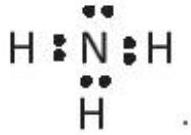
\includegraphics[width=\textwidth]{2025_10_23_daab5c8457c85b365b9eg-25}
\end{center}
\end{figure}

B.\\
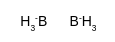
\includegraphics{smile-aa7a8abd3fa2e635398434bc8338ea526de69aef}

C.\\
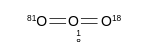
\includegraphics{smile-64cac004bef7980918624e4cec81e76728478487}

D.\\
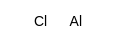
\includegraphics{smile-bef21e608748f21dbf05933718c9022cd676912e}

\section*{THÔNG HIỂU}
10.5. Trong công thức $C S_{2}$, tổng số cặp electron lớp ngoài cùng của C và S chưa tham gia liên kết là\\
A. 2 .\\
B. 3 .\\
C. 4.\\
D. 5 .\\
10.6. Phân tử nào sau đây có các nguyên tử đều đã đạt cấu hình electron bão hoà theo quy tắc octet?\\
A. $\mathrm{BeH}_{2}$.\\
B. $\mathrm{AlCl}_{3}$.\\
C. $\mathrm{PCl}_{5}$.\\
D. $\mathrm{SiF}_{4}$\\
10.7. Quy tắc octet không đúng với trường hợp phân tử chất nào sau đây?\\
A. $\mathrm{H}_{2} \mathrm{O}$.\\
B. $\mathrm{NO}_{2}$.\\
C. $\mathrm{CO}_{2}$.\\
D. $\mathrm{Cl}_{2}$.\\
10.8. Trong tự nhiên, các khí hiếm tồn tại dưới dạng nguyên tử tự do. Các nguyên tử của khí hiếm không liên kết với nhau tạo thành phân tử và rất khó liên kết với các nguyên tử của các nguyên tố khác. Ngược lại nguyên tử các nguyên tố khác lại liên kết với nhau tạo thành phân tử hay tinh thể. Giải thích.\\
10.9. Cấu hình electron lớp ngoài cùng của nguyên tử potassium (kali) là $4 \mathrm{~s}^{1}$, cấu hình electron lớp ngoài cùng của nguyên tử bromine là $4 \mathrm{~s}^{2} 4 \mathrm{p}^{5}$. Làm thế nào các nguyên tử potassium và bromine có được cấu hình electron của nguyên tử khí hiếm theo quy tắc octet.\\
10.10. Khi hình thành liên kết $\mathrm{H}+\mathrm{Cl} \rightarrow \mathrm{HCl}$ và khi phá vỡ liên kết $\mathrm{HCl} \rightarrow \mathrm{H}+\mathrm{Cl}$ thì hệ thu năng lượng hay toả năng lượng. Năng lượng phân tử HCl lớn hơn hay nhỏ hơn năng lượng hệ hai nguyên tử H và Cl riêng rẽ? Trong hai hệ đó thì hệ nào bền hơn?\\
10.11. Trong phân tử $\mathrm{Na}_{2} \mathrm{~S}$, cấu hình electron của các nguyên tử có tuân theo quy tắc octet không?

\section*{VẬN DỤNG}
10.12. Vận dụng quy tắc octet để giải thích sự hình thành liên kết trong các phân tử: $\mathrm{O}_{2}, \mathrm{CO}_{2}, \mathrm{CaCl}_{2}, \mathrm{KBr}$.\\
10.13. Đá vôi (thành phần chính là $\mathrm{CaCO}_{3}$ ) được dùng để sản xuất vôi, trong lĩnh vực xây dựng,... Barium nitrate $\mathrm{Ba}\left(\mathrm{NO}_{3}\right)_{2}$ có trong thành phần của kính quang học, gốm, men,... Phèn đơn aluminium sulfate (thành phần chính là $\mathrm{Al}_{2}\left(\mathrm{SO}_{4}\right)_{3}$ ) được sử dưng rộng rãi trong xử lí nước thải, trong công nghệ sản xuất giấy, công nghệ nhuộm vải và công nghệ lọc nước và nuôi trồng thuỷ sản,... Dựa vào quy tắc octet, đề xuất công thức cấu tạo của các chất trên.\\
10.14. Hợp chất $X$ tạo bởi hai nguyên tố $A, D$ có khối lượng phân tử là $76 . X$ là dung môi không phân cực, thường được sử dựng làm nguyên liệu trong tổng hợp chất hữu cơ chứa lưu huỳnh và được sử dụng rộng rãi trong sản xuất vải viscoza mềm. A có công thức hydride dạng $\mathrm{AH}_{4}$ và D có công thức oxide ứng với hoá trị cao nhất dạng $\mathrm{DO}_{3}$.\\
a) Hãy thiết lập công thức phân tử của X . Biết rằng A có số oxi hoá cao nhất trong X .\\
b) Đề xuất công thức cấu tạo của X và cho biết các nguyên tử thành phần của X khi liên kết có đủ electron theo quy tắc octet không.

\section*{Bài 11. LIÊN KẾT ION}
\section*{NHẬN BIÉT}
11.1. Liên kết ion được tạo thành giữa hai nguyên tử bằng\\
A. một hay nhiều cặp electron dùng chung.\\
B. một hay nhiều cặp electron dùng chung chỉ do một nguyên tử đóng góp.\\
C. lực hút tĩnh điện giữa các ion mang điện tích trái dấu.\\
D. một hay nhiều cặp electron dùng chung và các cặp electron này lệch về nguyên tử có độ âm điện lớn hơn.\\
11.2. Liên kết ion là loại liên kết hoá học được hình thành nhờ lực hút tĩnh điện giữa các phần tử nào sau đây?\\
A. cation và anion.\\
B. các anion.\\
C. cation và electron tự do.\\
D. electron và hạt nhân nguyên tử.\\
11.3. Biểu diễn sự tạo thành ion nào sau đây đúng?\\
A. $\mathrm{Na}+\mathrm{le} \rightarrow \mathrm{Na}^{+}$.\\
B. $\mathrm{Cl}_{2} \rightarrow 2 \mathrm{Cl}^{-}+2 \mathrm{e}$.\\
C. $\mathrm{O}_{2}+2 \mathrm{e} \rightarrow 2 \mathrm{O}^{2-}$.\\
D. $\mathrm{Al} \rightarrow \mathrm{Al}^{3+}+3 \mathrm{e}$.\\
11.4. Số electron và số proton trong ion $\mathrm{NH}_{4}^{+}$là\\
A. 11 electron và 11 proton.\\
B. 10 electron và 11 proton.\\
C. 11 electron và 10 proton.\\
D. 11 electron và 12 proton.\\
11.5. Cặp nguyên tử nào sau đây không tạo hợp chất dạng $\mathrm{X}_{2}^{+} \mathrm{Y}^{2-}$ hoặc $\mathrm{X}^{2+} \mathrm{Y}_{2}^{-}$?\\
A. Na và O .\\
B. K và S .\\
C. Ca và O .\\
D. Ca và Cl .\\
11.6. Tính chất nào sau đây là tính chất của hợp chất ion?\\
A. Hợp chất ion có nhiệt độ nóng chảy thấp.\\
B. Hợp chất ion có nhiệt độ nóng chảy cao.\\
C. Hợp chất ion dễ hoá lỏng.\\
D. Hợp chất ion có nhiệt độ sôi không xác định.

\section*{THÔNG HIỂU}
11.7. Cho các phân tử sau: $\mathrm{HCl}, \mathrm{NaCl}, \mathrm{CaCl}_{2}, \mathrm{AlCl}_{3}$.

Phân tử có liên kết mang nhiều tính chất ion nhất là\\
A. HCl .\\
B. NaCl .\\
C. $\mathrm{CaCl}_{2}$.\\
D. $\mathrm{AlCl}_{3}$.\\
11.8. Dãy gồm các phân tử đều có liên kết ion là\\
A. $\mathrm{Cl}_{2}, \mathrm{Br}_{2}, \mathrm{I}_{2}, \mathrm{HCl}$.\\
B. $\mathrm{HCl}, \mathrm{H}_{2} \mathrm{~S}, \mathrm{NaCl}, \mathrm{N}_{2} \mathrm{O}$.\\
C. $\mathrm{Na}_{2} \mathrm{O}, \mathrm{KCl}, \mathrm{BaCl}_{2}, \mathrm{Al}_{2} \mathrm{O}_{3}$.\\
D. $\mathrm{MgO}, \mathrm{H}_{2} \mathrm{SO}_{4}, \mathrm{H}_{3} \mathrm{PO}_{4}, \mathrm{HCl}$.\\
11.9. Cho các ion sau: $\mathrm{K}^{+} ; \mathrm{Be}^{2+} ; \mathrm{Cr}^{3+} ; \mathrm{F}^{-} ; \mathrm{Se}^{2-} ; \mathrm{N}^{3-}$.

Viết phương trình biểu diễn sự hình thành mỗi ion trên.\\
11.10. Cho các ion sau: $20 \mathrm{Ca}^{2+} ; 13 \mathrm{Al}^{3+} ; 9 \mathrm{~F}^{-} ; 16 \mathrm{~S}^{2-} ; 7 \mathrm{~N}^{3-}$.\\
a) Viết cấu hình electron của mỗi ion.\\
b) Mỗi cấu hình đă viết giống với cấu hình electron của nguyên tử nào?\\
11.11. Vì sao các hợp chất ion thường là chất rắn ở nhiệt độ phòng?\\
11.12. Cho các chất sau: $\mathrm{K}_{2} \mathrm{O}, \mathrm{H}_{2} \mathrm{O}, \mathrm{H}_{2} \mathrm{~S}, \mathrm{SO}_{2}, \mathrm{NaCl}, \mathrm{K}_{2} \mathrm{~S}, \mathrm{CaF}_{2}, \mathrm{HCl}$. Trong phân tử chất nào có liên kết ion?\\
11.13. Kể ra những hợp chất ion tạo thành từ các ion sau: $\mathrm{F}^{-}, \mathrm{K}^{+}, \mathrm{O}^{2-}, \mathrm{Ca}^{2+}$.

\section*{VẬN DỤNG}
11.14. Dùng sơ đồ để biểu diễn sự hình thành liên kết trong mỗi hợp chất ion sau đây:\\
a) magnesium fluoride $\left(\mathrm{MgF}_{2}\right)$;\\
b) potassium fluoride (KF);\\
c) sodium oxide ( $\mathrm{Na}_{2} \mathrm{O}$ );\\
d) calcium oxide ( CaO ).\\
11.15. Anion $\mathrm{X}^{-}$có cấu hình electron nguyên tử ở phân lớp ngoài cùng là $3 \mathrm{p}^{6}$.\\
a) Viết cấu hình electron của nguyên tử X . Cho biết X là nguyên tố kim loại hay phi kim.\\
b) Giải thích bản chất liên kết giữa X với barium.\\
11.16. Nguyên tố X tích luỹ trong các tế bào thực vật nên rau và trái cây tươi là nguồn cung cấp tốt nguyên tố X cho cơ thể. Các nghiên cứu chỉ ra khẩu phần ăn chứa nhiều X có thể giảm nguy cơ cao huyết áp và đột quỵ. Nguyên tố Z được dùng chế tạo dược phẩm, phẩm nhuộm và chất nhạy với ánh sáng. Nguyên tử $X$ chỉ có 7 electron trên phân lớp s ; còn nguyên tử Z chỉ có 17 electron trên phân lớp p .\\
a) Viết công thức hoá học của hợp chất tạo bởi $X$ và $Z$.\\
b) Hợp chất tạo bởi X và Z có tính dẫn điện không? Vì sao?\\
c) Trong thực tế cuộc sông, hợp chất tạo bởi X và Z được dùng để làm gi ?

\section*{Bài 12. LIÊN KẾT CỘNG HOÁ TR!}
\section*{NHẬN BIÉT}
12.1. Liên kết cộng hoá trị là liên kết hoá học được hình thành giữa hai nguyên tử bằng\\
A. một electron chung.\\
B. sự cho - nhận electron.\\
C. một cặp electron góp chung.\\
D. một hay nhiều cặp electron dùng chung.\\
12.2. Hợp chất nào sau đây có liên kết cộng hoá trị không phân cực?\\
A. LiCl .\\
B. $\mathrm{CF}_{2} \mathrm{Cl}_{2}$.\\
C. $\mathrm{CHCl}_{3}$.\\
D. $\mathrm{N}_{2}$.\\
12.3. Hợp chất nào sau đây có liên kết cộng hoá trị phân cực?\\
A. $\mathrm{H}_{2}$.\\
B. $\mathrm{CHCl}_{3}$.\\
C. $\mathrm{CH}_{4}$.\\
D. $\mathrm{N}_{2}$.\\
12.4. Liên kết $\sigma$ là liên kết hình thành do\\
A. sự xen phủ bên của hai orbital.\\
B. cặp electron dùng chung.\\
C. lực hút tĩnh điện giữa hai ion.\\
D. sự xen phủ trục của hai orbital.\\
12.5. Liên kết $\pi$ là liên kết hình thành do\\
A. sự xen phủ bên của hai orbital.\\
B. cặp electron dùng chung.\\
C. lực hút tĩnh điện giữa hai ion.\\
D. sự xen phủ trục của hai orbital.\\
12.6. Liên kết trong phân tử nào sau đây được hình thành nhờ sự xen phủ orbital $\mathrm{p}-\mathrm{p}$ ?\\
A. $\mathrm{H}_{2}$.\\
B. $\mathrm{Cl}_{2}$.\\
C. $\mathrm{NH}_{3}$.\\
D. HCl .\\
12.7. Liên kết trong phân tử nào sau đây được hình thành nhờ sự xen phủ orbital $\mathrm{s}-\mathrm{s}$ ?\\
A. $\mathrm{H}_{2}$.\\
B. $\mathrm{Cl}_{2}$.\\
C. $\mathrm{NH}_{3}$.\\
D. HCl .\\
12.8. Liên kết trong phân tử nào sau đây được hình thành nhờ sự xen phủ orbital $\mathrm{s}-\mathrm{p}$ ?\\
A. $\mathrm{H}_{2}$.\\
B. $\mathrm{Cl}_{2}$.\\
C. $\mathrm{NH}_{3}$.\\
D. $\mathrm{O}_{2}$.

\section*{THÔNG HIỂU}
12.9. Các liên kết trong phân tử oxygen gồm\\
A. 2 liên kết $\pi$.\\
B. 2 liên kết $\sigma$.\\
C. 1 liên kết $\sigma, 1$ liên kết $\pi$.\\
D. 1 liên kết $\sigma$.\\
12.10. Số liên kết $\sigma$ và $\pi$ có trong phân tử $\mathrm{C}_{2} \mathrm{H}_{2}$ lần lượt là\\
A. 2 và 3 .\\
B. 3 và 1 .\\
C. 2 và 2 .\\
D. 3 và 2 .\\
12.11. Dãy nào sau đây gồm các chất chỉ có liên kết cộng hoá trị?\\
A. $\mathrm{BaCl}_{2}, \mathrm{NaCl}, \mathrm{NO}_{2}$.\\
B. $\mathrm{SO}_{2}, \mathrm{CO}_{2}, \mathrm{Na}_{2} \mathrm{O}_{2}$.\\
C. $\mathrm{SO}_{3}, \mathrm{H}_{2} \mathrm{~S}, \mathrm{H}_{2} \mathrm{O}$.\\
D. $\mathrm{CaCl}_{2}, \mathrm{~F}_{2} \mathrm{O}, \mathrm{HCl}$.\\
12.12. Cho hai nguyên tố $X(Z=20)$ và $Y(Z=17)$. Công thức hợp chất tạo thành từ nguyên tố $\mathrm{X}, \mathrm{Y}$ và liên kết trong phân tử là\\
A. XY : liên kết cộng hoá trị.\\
B. $\mathrm{X}_{2} \mathrm{Y}_{3}$ : liên kết cộng hoá trị.\\
C. $X_{2} Y$ : liên kết ion.\\
D. $\mathrm{XY}_{2}$ : liên kết ion.\\
12.13. Độ âm điện của nitrogen gần bằng độ âm điện của chlorine nhưng ở điều kiện thường $\mathrm{N}_{2}$ hoạt động kém $\mathrm{Cl}_{2}$. Giải thích.

\section*{VÂN DỤNG}
12.14. Cho các phân tử sau: $\mathrm{F}_{2}, \mathrm{~N}_{2}, \mathrm{H}_{2} \mathrm{O}, \mathrm{CO}_{2}$.\\
a) Hãy viết công thức Lewis của các phân tử đó.\\
b) Hãy cho biết phân tử nào chứa liên kết cộng hoá trị phân cực và phân tử nào chứa liên kết cộng hoá trị không phân cực; phân tử nào phân cực và phân tử nào không phân cực.\\
12.15. Cho các phân tử sau: $\mathrm{Br}_{2}, \mathrm{H}_{2} \mathrm{~S}, \mathrm{CH}_{4}, \mathrm{NH}_{3}, \mathrm{C}_{2} \mathrm{H}_{4}, \mathrm{C}_{2} \mathrm{H}_{2}$.\\
a) Phân tử nào có liên kết cộng hoá trị không phân cực? Phân tử nào có liên kết cộng hoá trị phân cực?\\
b) Phân tử nào chỉ có liên kết đơn? Phân tử nào có liên kết đôi? Phân tử nào có liên kết ba?\\
12.16. Ghép nhiệt độ nóng chảy với chất tương ứng và giải thích.

\begin{center}
\begin{tabular}{|l|l|}
\hline
Chất & Nhiệt độ nóng chảy ( ${ }^{\circ} \mathrm{C}$ ) \\
\hline
a) Nước & 1) -138 \\
\hline
b) Muối ăn & 2) 80 \\
\hline
c) Băng phiến & 3) 0 \\
\hline
d) Butane & 4) 801 \\
\hline
\end{tabular}
\end{center}

\section*{Bài 13. LIÊN KẾT HYDROGEN VÀ TƯƠNG TÁC VAN DER WAALS}
\section*{NHẬN BIẾT}
13.1. Liên kết hydrogen là loại liên kết hoá học được hình thành giữa các nguyên tử nào sau đây?\\
A. Phi kim và hydrogen trong hai phân tử khác nhau.\\
B. Phi kim và hydrogen trong cùng một phân tử.\\
C. Phi kim có độ âm điện lớn và nguyên tử hydrogen.\\
D. $\mathrm{F}, \mathrm{O}, \mathrm{N}, \ldots$ có độ âm điện lớn, đồng thời có cặp electron hoá trị chưa liên kết và nguyên tử hydrogen linh động.\\
13.2. Tương tác van der Waals được hình thành do\\
A. tương tác tĩnh điện lưỡng cực - lưỡng cực giữa các nguyên tử.\\
B. tương tác tĩnh điện lưỡng cực - lưỡng cực giữa các phân tử.\\
C. tương tác tĩnh điện lưỡng cực - lưỡng cực giữa các nguyên tử hay phân tử.\\
D. lực hút tĩnh điện giữa các phân tử phân cực.\\
13.3. Chất nào sau đây có thể tạo liên kết hydrogen?\\
A. $\mathrm{PF}_{3}$.\\
B. $\mathrm{CH}_{4}$.\\
C. $\mathrm{CH}_{3} \mathrm{OH}$.\\
D. $\mathrm{H}_{2} \mathrm{~S}$.\\
13.4. Chất nào sau đây không thể tạo được liên kết hydrogen?\\
A. $\mathrm{H}_{2} \mathrm{O}$.\\
B. $\mathrm{CH}_{4}$.\\
C. $\mathrm{CH}_{3} \mathrm{OH}$.\\
D. $\mathrm{NH}_{3}$.\\
13.5. Tương tác van der Waals tồn tai giữa những\\
A. ion.\\
B. hạt proton.\\
C. hạt neutron.\\
D. phân tử.\\
13.6. Cho các chất sau: $\mathrm{F}_{2}, \mathrm{Cl}_{2}, \mathrm{Br}_{2}, \mathrm{I}_{2}$.

Chất có nhiệt độ nóng chảy thấp nhất là\\
A. $F_{2}$\\
B. $\mathrm{Cl}_{2}$.\\
C. $\mathrm{Br}_{2}$.\\
D. $\mathrm{I}_{2}$.\\
13.7. Cho các chất sau: $\mathrm{F}_{2}, \mathrm{Cl}_{2}, \mathrm{Br}_{2}, \mathrm{I}_{2}$.

Chất có nhiệt độ sôi cao nhất là\\
A. $F_{2}$.\\
B. $\mathrm{Cl}_{2}$.\\
C. $\mathrm{Br}_{2}$.\\
D. $\mathrm{I}_{2}$.\\
13.8. Dãy chất nào sau đây xếp theo thứ tự nhiệt độ sôi tăng dần?\\
A. $\mathrm{H}_{2} \mathrm{O}, \mathrm{H}_{2} \mathrm{~S}, \mathrm{CH}_{4}$.\\
B. $\mathrm{H}_{2} \mathrm{~S}, \mathrm{CH}_{4}, \mathrm{H}_{2} \mathrm{O}$.\\
C. $\mathrm{CH}_{4}, \mathrm{H}_{2} \mathrm{O}, \mathrm{H}_{2} \mathrm{~S}$.\\
D. $\mathrm{CH}_{4}, \mathrm{H}_{2} \mathrm{~S}, \mathrm{H}_{2} \mathrm{O}$.

\section*{THÔNG HIỂU}
13.9. Cho các khí hiếm sau: $\mathrm{He}, \mathrm{Ne}, \mathrm{Ar}, \mathrm{Kr}, \mathrm{Xe}$.

Khí hiếm có nhiệt độ nóng chảy thấp nhất và cao nhất lần lượt là\\
A. Xe và He .\\
B. Ar và Ne .\\
C. He và Xe.\\
D. He và Kr .\\
13.10. Cho các chất sau: $\mathrm{C}_{2} \mathrm{H}_{6} ; \mathrm{H}_{2} \mathrm{O} ; \mathrm{NH}_{3} ; \mathrm{PF}_{3} ; \mathrm{C}_{2} \mathrm{H}_{5} \mathrm{OH}$. Số chất tạo được liên kết hydrogen là\\
A. 2 .\\
B. 3 .\\
C. 4 .\\
D. 5 .\\
13.11. Giữa $\mathrm{H}_{2} \mathrm{O}$ và HF có thể tạo ra it nhất bao nhiêu kiểu liên kết hydrogen?\\
A. 2 .\\
B. 3 .\\
C. 4 .\\
D. 5 .\\
13.12. Nhiệt độ sôi của từng chất methane, ethane, propane và butane là một trong bốn nhiệt độ sau: $0^{\circ} \mathrm{C} ;-164^{\circ} \mathrm{C} ;-42^{\circ} \mathrm{C}$ và $-88^{\circ} \mathrm{C}$. Nhiệt độ sôi $-88^{\circ} \mathrm{C}$ là của chất nào sau đây?\\
A. methane.\\
B. propane.\\
C. ethane.\\
D. butane.\\
13.13. Cho các chất sau: $\mathrm{C}_{2} \mathrm{H}_{6} ; \mathrm{CH}_{3} \mathrm{OH} ; \mathrm{CH}_{3} \mathrm{COOH}$.

Chất nào có thể tạo được liên kết hydrogen? Vì sao?\\
13.14. Khối lượng $\mathrm{mol}(\mathrm{g} / \mathrm{mol})$ của nước, ammonia và methane lần lượt bằng 18,17 và 16. Nước sôi ở $100^{\circ} \mathrm{C}$, còn ammonia sôi ở $-33,35^{\circ} \mathrm{C}$ và methane sôi ở $-161,58^{\circ} \mathrm{C}$. Giải thích vì sao các chất trên có khối lượng mol xấp xỉ nhau nhưng nhiệt độ sôi của chúng lại chênh lệch nhau.

\section*{VẬN DỤNG}
13.15. Trong dung dịch ethanol $\left(\mathrm{C}_{2} \mathrm{H}_{5} \mathrm{OH}\right)$ có những kiểu liên kết hydrogen nào? Kiểu nào bền nhất và kém bền nhất? Mô tả bằng hình vẽ.\\
13.16. Trong phân tử nước và ammonia, phân tử nào có thể tạo nhiều liên kết hydrogen hơn? Vì sao?\\
13.17. Dầu mỏ chứa hỗn hợp nhiều hydrocarbon như: octane $\left(\mathrm{C}_{8} \mathrm{H}_{18}\right)$ có trong xăng; butane $\left(\mathrm{C}_{4} \mathrm{H}_{10}\right)$ có trong gas. Khi chưng cất dầu mỏ, octane hay butane sẽ bay hơi trước? Giải thích.\\
13.18. Cho các chất và các trị số nhiệt độ sôi $\left({ }^{\circ} \mathrm{C}\right)$ sau: $\mathrm{H}_{2} \mathrm{O}, \mathrm{H}_{2} \mathrm{~S}, \mathrm{H}_{2} \mathrm{Se}, \mathrm{H}_{2} \mathrm{Te}$ và $-42 ;-2 ; 100 ;-61$.\\
Ghép các trị số nhiệt độ sôi vào mỗi chất sao cho phù hợp và giải thích.

\section*{Bài 14. ÔN TẬP CHƯƠNG 3}
\section*{NHẬN BIÉT}
14.1. Quy tắc octet không đúng với trường hợp phân tử chất nào sau đây?\\
A. $\mathrm{H}_{2} \mathrm{~S}$.\\
B. $\mathrm{PCl}_{5}$.\\
C. $\mathrm{SiO}_{2}$.\\
D. $\mathrm{Br}_{2}$.\\
14.2. Phát biểu nào sau đây không đúng về liên kết có trong phân tử HCl ?\\
A. Giữa nguyên tử H và Cl có một liên kết đơn.\\
B. Các electron tham gia liên kết đồng thời bị hút về phía hai hạt nhân.\\
C. Phân tử có một momen lưỡng cực.\\
D. Một electron của nguyên tử hydrogen và một electron của nguyên tử chlorine được góp chung và cách đều hai nguyên tử.\\
14.3. Liên kết ion khác với liên kết cộng hoá trị ở điểm nào sau đây?\\
A. Tính bão hoà lớp electron ở vỏ nguyên tử.\\
B. Tuân theo quy tắc octet.\\
C. Tạo ra hợp chất bền vững hơn.\\
D. Tính không định hướng.\\
14.4. Cho chất hữu cơ A có công thức cấu tạo sau:\\
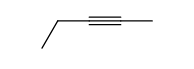
\includegraphics{smile-3ebd5113c46e76d4b747ac128c0dac6bcfd60367}

Số liên kết $\sigma$ trong phân tử A là\\
A. 6 .\\
B. 8 .\\
C. 9 .\\
D. 11 .\\
14.5. Cho giá trị độ âm điện của một số nguyên tố sau: $\mathrm{Na}(0,93) ; \mathrm{Li}(0,98)$; $\mathrm{Mg}(1,31) ; \mathrm{Al}(1,61) ; \mathrm{P}(2,19) ; \mathrm{S}(2,58) ; \mathrm{Br}(2,96)$ và $\mathrm{Cl}(3,16)$. Phân tử nào sau đây có liên kết ion?\\
A. $\mathrm{Na}_{3} \mathrm{P}$.\\
B. MgS .\\
C. $\mathrm{AlCl}_{3}$.\\
D. LiBr .\\
14.6. Cho hai chất hữu cơ X và Y có công thức cấu tạo sau:\\
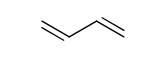
\includegraphics{smile-0b352f25a70ec0798b6ee6fc501bd3194b845cec}

(X)\\
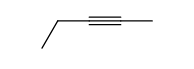
\includegraphics{smile-e9d0bffc73de7f89a010f40db89a7c535810b02c}

(Y)

Nhận xét nào sau đây là đúng?\\
A. $X$ và $Y$ có số liên kết $\sigma$ và số liên kết $\pi$ bằng nhau.\\
B. X có số liên kết $\sigma$ và số liên kết $\pi$ nhiều hơn Y .\\
C. $X$ có số liên kết $\sigma$ nhiều hơn, nhưng số liên kết $\pi$ it hơn $Y$.\\
D. $X$ có số liên kết $\sigma$ it hơn, nhưng số liên kết $\pi$ nhiều hơn $Y$.\\
14.7. Nguyên tố X ở nhóm IA và nguyên tố Y ở nhóm VIIA của bảng tuần hoàn. X và $Y$ có thể tạo thành hợp chất $R$. Liên kết giữa các nguyên tử trong $R$ thuộc loại liên kết nào sau đây?\\
A. Ion.\\
B. Cộng hoá trị phân cực.\\
C. Cộng hoá trị không phân cực.\\
D. Hydrogen.

\section*{THÔNG HIỂU}
14.8. $\mathrm{X}, \mathrm{Y}, \mathrm{Z}$ là những nguyên tố có số hiệu nguyên tử lần lượt là $8,19,16$. Các cặp nguyên tố có thể tạo thành liên kết ion và cộng hoá trị phân cực lần lượt là\\
A. $(\mathrm{X}, \mathrm{Y}) ;(\mathrm{X}, \mathrm{Z})$ và $(\mathrm{Y}, \mathrm{Z})$.\\
B. $(\mathrm{X}, \mathrm{Z}) ;(\mathrm{Y}, \mathrm{Z})$ và $(\mathrm{X}, \mathrm{Y})$.\\
C. $(\mathrm{X}, \mathrm{Y}) ;(\mathrm{Y}, \mathrm{Z})$ và $(\mathrm{X}, \mathrm{Z})$.\\
D. $(\mathrm{Z}, \mathrm{Y}) ;(\mathrm{Y}, \mathrm{X})$ và $(\mathrm{X}, \mathrm{Z})$.\\
14.9. Cho các chất sau: $\mathrm{N}_{2}, \mathrm{H}_{2}, \mathrm{NH}_{3}, \mathrm{NaCl}, \mathrm{HCl}, \mathrm{H}_{2} \mathrm{O}$.

Số chất mà phân tử chỉ chứa liên kết cộng hoá trị không phân cực là\\
A. 2 .\\
B. 4 .\\
C. 5.\\
D. 3 .\\
14.10. Cho các chất sau: (1) $\mathrm{H}_{2} \mathrm{~S}$;\\
(2) $\mathrm{SO}_{2}$;\\
(3) NaCl ;\\
(4) CaO ;\\
(5) $\mathrm{NH}_{3}$; (6) $\mathrm{HBr} ; \quad$ (7) $\mathrm{CO}_{2} ; \quad$ (8) $\mathrm{K}_{2} \mathrm{~S}$.

Dãy nào sau đây gồm các chất có liên kết cộng hoá trị?\\
A. (1); (2); (3); (4); (7).\\
B. (1); (2); (5); (6); (7).\\
C. (1); (3); (5); (6); (7).\\
D. (1); (2); (5); (7); (8).\\
14.11. Dùng công thức Lewis để biểu diễn phân tử $\mathrm{SO}_{3}$ sao cho phù hợp với quy tắc octet. Chỉ rõ các liên kết trong phân tử thuộc loại liên kết nào.\\
14.12. Hợp chất NaClO là thành phần của chất tẩy rửa, sát trùng có tên gọi là "Nước Javen". Áp dụng quy tắc octet để giải thích sự hình thành các liên kết trong hợp chất đó.

\section*{VẬN DỤNG}
14.13. Tính số liên kết $\sigma$ và liên kết $\pi$ trong các phân tử sau:\\
a) $\mathrm{C}_{2} \mathrm{H}_{4}$;\\
b) $\mathrm{C}_{2} \mathrm{H}_{2}$;\\
c) HCN ;\\
d) HCOOH .\\
14.14. Dựa vào giá trị của độ âm điện ở Bảng 6.2 trong sách giáo khoa Hoá học 10, hãy nêu bản chất liên kết trong các phân tử và ion sau: HClO , $\mathrm{KHS}, \mathrm{HCO}_{3}^{-}, \mathrm{K}_{2} \mathrm{SO}_{4}$.\\
14.15. Cho dãy các chất kèm theo nhiệt độ sôi $\left({ }^{\circ} \mathrm{C}\right)$ sau:

$$
\mathrm{HF}(19,5) ; \mathrm{HCl}(-85) ; \mathrm{HBr}(-66) ; \mathrm{HI}(-35)
$$

a) Nêu xu hướng biến đổi nhiệt độ sôi trong dãy chất trên.\\
b) Đề xuất lí do nhiệt độ sôi của HF không theo xu hướng này.\\
14.16. Cho biết tổng số electron trong anion $\mathrm{AB}_{3}^{2-}$ là 42. Trong các hạt nhân A cũng như B có số proton bằng số neutron.\\
a) Tính số khối của $A, B$.\\
b) Đề xuất cấu tạo Lewis cho anion $\mathrm{AB}_{3}^{2-}$ sao cho phù hợp với quy tắc octet.\\
14.17. Hợp chất X được sử dụng làm thuốc pháo, ngòi nổ, thuốc đầu diêm, thuốc giúp nhãn ra hoa,... X có khối lượng mol bằng $122,5 \mathrm{~g} / \mathrm{mol}$, chứa ba nguyên tố, trong đó nguyên tố s có 7 electron s, nguyên tố p có 11 electron p và nguyên tố p có 4 electron p . Thành phần phần trăm khối lượng nguyên tố có 4 electron p trong X bằng $39,19 \%$.\\
a) Xác định công thức phân tử của X .\\
b) Viết công thức cấu tạo Lewis, chỉ rõ loại liên kết có trong $X$.

\section*{CHUONG 4 PHẢN ÚNG OXI HOÁ - KHƯ}
\section*{Bài 15. PHẢN ÚNG OXI HOÁ - KHƯ}
\section*{NHẬN BIẾT}
15.1. Số oxi hoá là một số đại số đặc trưng cho đại lượng nào sau đây của nguyên tử trong phân tử?\\
A. Hoá trị.\\
B. Điện tích.\\
C. Khối lượng.\\
D. Số hiệu.\\
15.2. Trong hợp chất $\mathrm{SO}_{3}$, số oxi hoá của sulfur (lưu huỳnh) là\\
A. +2 .\\
B. +3 .\\
C. +5 .\\
D. +6 .\\
15.3. $\mathrm{Fe}_{2} \mathrm{O}_{3}$ là thành phần chính của quặng hematite đỏ, dùng để luyện gang. Số oxi hoá của iron (sắt) trong $\mathrm{Fe}_{2} \mathrm{O}_{3}$ là\\
A. +3 .\\
B. $3+$.\\
C. 3.\\
D. -3 .\\
15.4. Ammonia $\left(\mathrm{NH}_{3}\right)$ là nguyên liệu để sản xuất nitric acid và nhiều loại phân bón. Số oxi hoá của nitrogen trong ammonia là\\
A. 3 .\\
B. 0 .\\
C. +3 .\\
D. -3 .\\
15.5. Chromium có số oxi hoá +2 trong hợp chất nào sau đây?\\
A. $\mathrm{Cr}(\mathrm{OH})_{3}$.\\
B. $\mathrm{Na}_{2} \mathrm{CrO}_{4}$.\\
C. $\mathrm{CrCl}_{2}$.\\
D. $\mathrm{Cr}_{2} \mathrm{O}_{3}$.\\
15.6. Phản ứng oxi hoá - khử là phản ứng có sự nhường và nhận\\
A. electron.\\
B. neutron.\\
C. proton.\\
D. cation.\\
15.7. Dấu hiệu để nhận ra một phản ứng oxi hoá - khử là dựa trên sự thay đổi đại lượng nào sau đây của nguyên tử?\\
A. Số khối.\\
B. Số oxi hoá.\\
C. Số hiệu.\\
D. Số mol.\\
15.8. Trong phản ứng oxi hoá - khử, chất oxi hoá là chất\\
A. nhường electron.\\
B. nhận electron.\\
C. nhận proton.\\
D. nhường proton.\\
15.9. Dẫn khí $\mathrm{H}_{2}$ đi qua ống sứ đựng bột CuO nung nóng để thực hiện phản ứng hoá học sau:

$$
\mathrm{CuO}+\mathrm{H}_{2} \xrightarrow{\mathrm{t}^{\circ}} \mathrm{Cu}+\mathrm{H}_{2} \mathrm{O} \text {. }
$$

Trong phản ứng trên, chất đóng vai trò chất khử là\\
A. CuO\\
B. Cu .\\
C. $\mathrm{H}_{2}$.\\
D. $\mathrm{H}_{2} \mathrm{O}$.\\
15.10. Phản ứng nào sau đây là phản ứng oxi hoá - khử?\\
A. $2 \mathrm{Ca}+\mathrm{O}_{2} \xrightarrow{\mathrm{t}^{\circ}} 2 \mathrm{CaO}$.\\
B. $\mathrm{CaCO}_{3} \xrightarrow{\mathrm{t}^{\circ}} \mathrm{CaO}+\mathrm{CO}_{2}$.\\
C. $\mathrm{CaO}+\mathrm{H}_{2} \mathrm{O} \longrightarrow \mathrm{Ca}(\mathrm{OH})_{2}$.\\
D. $\mathrm{Ca}(\mathrm{OH})_{2}+\mathrm{CO}_{2} \longrightarrow \mathrm{CaCO}_{3}+\mathrm{H}_{2} \mathrm{O}$.

\section*{THÔNG HIỂU}
15.11. Cho các chất sau: $\mathrm{Cl}_{2}, \mathrm{HCl}, \mathrm{NaCl}, \mathrm{KClO}_{3}, \mathrm{HClO}_{4}$.

Số oxi hoá của nguyên tử Cl trong phân tử các chất trên lần lượt là\\
A. $0 ;+1 ;+1 ;+5 ;+7$.\\
B. $0 ;-1 ;-1 ;+5 ;+7$.\\
C. $1 ;-1 ;-1 ;-5 ;-7$.\\
D. $0 ; 1 ; 1 ; 5 ; 7$.\\
15.12. Thuốc tím chứa ion permanganate $\left(\mathrm{MnO}_{4}^{-}\right)$có tính oxi hoá mạnh, được dùng để sát trùng, diệt khuẩn trong y học, đời sông và nuôi trồng thuỷ sản. Số oxi hoá của manganse trong ion permanganate là\\
A. +2 .\\
B. +3 .\\
C. +7.\\
D. +6 .\\
15.13. Cho các phân tử có công thức cấu tạo sau:\\
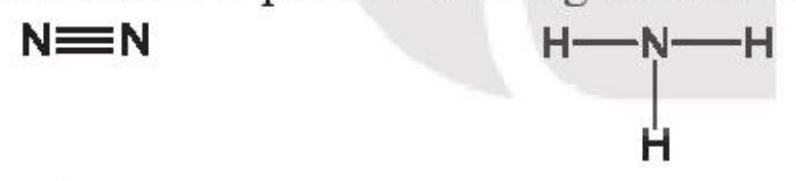
\includegraphics[max width=\textwidth, center]{2025_10_23_daab5c8457c85b365b9eg-37}\\
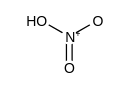
\includegraphics{smile-05a586121601408a2bcf8ebfbfb55f3298ad3186}

Số oxi hoá của nguyên tử N trong các phân tử trên lần lượt là\\
A. $0 ;-3 ;-4$.\\
B. $0 ;+3 ;+5$.\\
C. $-3 ;-3 ;+4$.\\
D. $0 ;-3 ;+5$.\\
15.14. Carbon đóng vai trò chất oxi hoá ở phản ứng nào sau đây?\\
A. $\mathrm{C}+\mathrm{O}_{2} \xrightarrow{\mathrm{t}^{\circ}} \mathrm{CO}_{2}$.\\
B. $\mathrm{C}+\mathrm{CO}_{2} \xrightarrow{\mathrm{t}^{\circ}} 2 \mathrm{CO}$.\\
C. $\mathrm{C}+\mathrm{H}_{2} \mathrm{O} \xrightarrow{\mathrm{t}^{\circ}} \mathrm{CO}+\mathrm{H}_{2}$.\\
D. $\mathrm{C}+2 \mathrm{H}_{2} \xrightarrow{\mathrm{t}^{\circ}} \mathrm{CH}_{4}$.\\
15.15. Thực hiện các phản ứng hoá học sau:\\
(a) $\mathrm{S}+\mathrm{O}_{2} \xrightarrow{\mathrm{t}^{\circ}} \mathrm{SO}_{2}$;\\
(b) $\mathrm{Hg}+\mathrm{S} \longrightarrow \mathrm{HgS}$;\\
(c) $\mathrm{H}_{2}+\mathrm{S} \xrightarrow{\mathrm{t}^{\circ}} \mathrm{H}_{2} \mathrm{~S}$;\\
(d) $\mathrm{S}+3 \mathrm{~F}_{2} \xrightarrow{\mathrm{t}^{\circ}} \mathrm{SF}_{6}$.

Số phản ứng sulfur đóng vai trò chất oxi hoá là\\
A. 4 .\\
B. 2 .\\
C. 3.\\
D. 1 .\\
15.16. Khi tham gia các phản ứng đốt cháy nhiên liệu, oxygen đóng vai trò là\\
A. chất khử.\\
B. acid.\\
C. chất oxi hoá.\\
D. base.\\
15.17. Chlorine vừa đóng vai trò chất oxi hoá, vừa đóng vai trò chất khử trong phản ứng nào sau đây?\\
A. $2 \mathrm{Na}+\mathrm{Cl}_{2} \xrightarrow{\mathrm{t}^{\circ}} 2 \mathrm{NaCl}$.\\
B. $\mathrm{H}_{2}+\mathrm{Cl}_{2} \xrightarrow{\text { as }} 2 \mathrm{HCl}$.\\
C. $2 \mathrm{FeCl}_{2}+\mathrm{Cl}_{2} \xrightarrow{\mathrm{t}^{\circ}} 2 \mathrm{FeCl}_{3}$.\\
D. $2 \mathrm{NaOH}+\mathrm{Cl}_{2} \longrightarrow \mathrm{NaCl}+\mathrm{NaClO}+\mathrm{H}_{2} \mathrm{O}$.\\
15.18. Cho các phản ứng hoá học sau:\\
(a) $\mathrm{CaCO}_{3} \xrightarrow{\mathrm{t}^{\circ}} \mathrm{CaO}+\mathrm{CO}_{2}$.\\
(b) $\mathrm{CH}_{4} \xrightarrow[\mathrm{xt}]{\mathrm{t}^{\circ}} \mathrm{C}+2 \mathrm{H}_{2}$.\\
(c) $2 \mathrm{Al}(\mathrm{OH})_{3} \xrightarrow{\mathrm{t}^{\circ}} \mathrm{Al}_{2} \mathrm{O}_{3}+3 \mathrm{H}_{2} \mathrm{O}$.\\
(d) $2 \mathrm{NaHCO}_{3} \xrightarrow{\mathrm{t}^{\circ}} \mathrm{Na}_{2} \mathrm{CO}_{3}+\mathrm{CO}_{2}+\mathrm{H}_{2} \mathrm{O}$.

Số phản ứng có kèm theo sự thay đổi số oxi hoá của các nguyên tử là\\
A. 2 .\\
B. 3 .\\
C. 1.\\
D. 4 .\\
15.19. Khí thiên nhiên nén ( CNG - Compressed Natural Gas) có thành phần chính là methane $\left(\mathrm{CH}_{4}\right)$, là nhiên liệu sạch, thân thiện với môi trường.\\
Xét phản ứng đốt cháy methane trong buồng đốt động cơ xe buýt sử dụng nhiên liệu $\mathrm{CNG}: \mathrm{CH}_{4}+\mathrm{O}_{2} \xrightarrow{\mathrm{t}^{\circ}} \mathrm{CO}_{2}+\mathrm{H}_{2} \mathrm{O}$.\\
a) Xác định các nguyên tử có sự thay đổi số oxi hoá. Viết quá trình oxi hoá, quá trình khử.\\
b) Lập phương trình hoá học của phản ứng theo phương pháp thăng bằng electron.\\
15.20. Xét phản ứng sản xuất $\mathrm{Cl}_{2}$ trong công nghiệp:

$$
\mathrm{NaCl}+\mathrm{H}_{2} \mathrm{O} \xrightarrow[\operatorname{mnx}]{\text { dpdd }} \mathrm{NaOH}+\mathrm{Cl}_{2}+\mathrm{H}_{2} .
$$

a) Xác định các nguyên tử có sự thay đổi số oxi hoá. Chỉ rõ chất oxi hoá, chất khử.\\
b) Lập phương trình hoá học của phản ứng theo phương pháp thăng bằng electron.

\section*{VÂN DỤNG}
15.21. Trên thế giới, zinc (kẽm) được sản xuất chủ yếu từ quặng zinc blende có thành phần chính là ZnS . Ở giai đoạn đầu của quá trình sản xuất, quặng zinc blende được nung trong không khí để thực hiện phản ứng:

$$
\mathrm{ZnS}+\mathrm{O}_{2} \xrightarrow{\mathrm{t}^{\circ}} \mathrm{ZnO}+\mathrm{SO}_{2}
$$

a) Xác định các nguyên tử có sự thay đổi số oxi hoá. Viết các quá trình oxi hoá, quá trình khử.\\
b) Lập phương trình hoá học của phản ứng theo phương pháp thăng bằng electron.\\
15.22. Khí đốt hoá lỏng thường gọi là gas, có thành phần gồm propane $\left(\mathrm{C}_{3} \mathrm{H}_{8}\right)$ và butane $\left(\mathrm{C}_{4} \mathrm{H}_{10}\right)$. Xét phản ứng đốt cháy butane khi đun bếp gas:

$$
\mathrm{C}_{4} \mathrm{H}_{10}+\mathrm{O}_{2} \xrightarrow{\mathrm{t}^{\circ}} \mathrm{CO}_{2}+\mathrm{H}_{2} \mathrm{O} .
$$

a) Xác định các nguyên tử có sự thay đổi số oxi hoá. Chỉ rõ chất oxi hoá, chất khử.\\
b) Lập phương trình hoá học của phản ứng theo phương pháp thăng bằng electron.\\
15.23. Hàm lượng iron(II) sulfate được xác định qua phản úng oxi hoá - khử với potassium permanganate:

$$
\mathrm{FeSO}_{4}+\mathrm{KMnO}_{4}+\mathrm{H}_{2} \mathrm{SO}_{4} \longrightarrow \mathrm{Fe}_{2}\left(\mathrm{SO}_{4}\right)_{3}+\mathrm{K}_{2} \mathrm{SO}_{4}+\mathrm{MnSO}_{4}+\mathrm{H}_{2} \mathrm{O}
$$

a) Lập phương trình hoá học của phản ưng theo phương pháp thăng bằng electron. Chỉ rõ chất oxi hoá, chất khử.\\
b) Tính thể tích dung dịch $\mathrm{KMnO}_{4} 0,02 \mathrm{M}$ để phản ứng vừa đủ với 20 mL dung dịch $\mathrm{FeSO}_{4} 0,10 \mathrm{M}$.\\
15.24. Cho $2,34 \mathrm{~g}$ kim loại M (hoá trị n ) tác dụng với dung dịch $\mathrm{H}_{2} \mathrm{SO}_{4}$ (đặc, nóng, dư) thu được $3,2227 \mathrm{~L}$ khí $\mathrm{SO}_{2}$ (điều kiện chuẩn). Xác định kim loại M .

\section*{Bài 16. ÔN TẬP CHƯƠNG 4}
\section*{NHẬN BIẾT}
16.1. Trong phản ứng oxi hoá - khử, chất nhường electron được gọi là\\
A. chất khử.\\
B. chất oxi hoá.\\
C. acid.\\
D. base.\\
16.2. Iron có số oxi hoá +2 trong hợp chất nào sau đây?\\
A. $\mathrm{Fe}(\mathrm{OH})_{3}$.\\
B. $\mathrm{FeCl}_{3}$.\\
C. $\mathrm{FeSO}_{4}$.\\
D. $\mathrm{Fe}_{2} \mathrm{O}_{3}$.\\
16.3. Chromium(VI) oxide, $\mathrm{CrO}_{3}$, là chất rắn, màu đỏ thẫm, vừa là acidic oxide, vừa là chất oxi hoá mạnh. Số oxi hoá của chromium trong oxide trên là\\
A. 0 .\\
B. +6 .\\
C. +2 .\\
D. +3 .\\
16.4. Phản ứng kèm theo sự cho và nhận electron được gọi là phản ứng\\
A. đốt cháy.\\
B. phân huỷ.\\
C. trao đồi.\\
D. oxi hoá - khử.\\
16.5. Xét phản ứng điều chế $\mathrm{H}_{2}$ trong phòng thí nghiệm:

$$
\mathrm{Zn}+2 \mathrm{HCl} \longrightarrow \mathrm{ZnCl}_{2}+\mathrm{H}_{2} .
$$

Chất đóng vai trò chất khử trong phản ứng là\\
A. $\mathrm{H}_{2}$.\\
B. $\mathrm{ZnCl}_{2}$.\\
C. HCl .\\
D. Zn .

\section*{THÔNG HIỂU}
16.6. Cho các hợp chất sau: $\mathrm{NH}_{3}, \mathrm{NH}_{4} \mathrm{Cl}, \mathrm{HNO}_{3}, \mathrm{NO}_{2}$.

Số hợp chất chứa nguyên tử nitrogen có số oxi hoá -3 là\\
A. 1 .\\
B. 3 .\\
C. 2 .\\
D. 4 .\\
16.7. Nguyên tử sulfur chỉ thể hiện tính khử trong chất nào sau đây?\\
A. S.\\
B. $\mathrm{SO}_{2}$.\\
C. $\mathrm{H}_{2} \mathrm{SO}_{4}$.\\
D. $\mathrm{H}_{2} \mathrm{~S}$.\\
16.8. Nguyên tử carbon vừa có khả năng thể hiện tính oxi hoá, vừa có khả năng thể hiện tính khử trong chất nào sau đây?\\
A. C.\\
B. $\mathrm{CO}_{2}$.\\
C. $\mathrm{CaCO}_{3}$.\\
D. $\mathrm{CH}_{4}$.\\
16.9. Hợp chất nào sau đây chứa hai loại nguyên tử iron với số oxi hoá +2 và +3 ?\\
A. FeO .\\
B. $\mathrm{Fe}_{3} \mathrm{O}_{4}$.\\
C. $\mathrm{Fe}(\mathrm{OH})_{3}$.\\
D. $\mathrm{Fe}_{2} \mathrm{O}_{3}$.\\
16.10. Cho các phân tử sau: $\mathrm{H}_{2} \mathrm{~S}, \mathrm{SO}_{3}, \mathrm{CaSO}_{4}, \mathrm{Na}_{2} \mathrm{~S}, \mathrm{H}_{2} \mathrm{SO}_{4}$. Số oxi hoá của nguyên tử S trong các phân tứ trên lần lượt là\\
A. $0 ;+6 ;+4 ;+4 ;+6$.\\
B. $0 ;+6 ;+4 ;+2 ;+6$.\\
C. $+2 ;+6 ;+6 ;-2 ;+6$.\\
D. $-2 ;+6 ;+6 ;-2 ;+6$.

\section*{VẬN DỤNG}
16.11. Trong công nghiệp, một lượng zinc được sản xuất theo phương pháp nhiệt luyện ở khoảng $1200^{\circ} \mathrm{C}$ theo phản ứng:

$$
\mathrm{ZnO}+\mathrm{C} \xrightarrow{\mathrm{t}^{\circ}} \mathrm{Zn}+\mathrm{CO}
$$

a) Xác định các nguyên tử có sự thay đổi số oxi hoá. Viết quá trình oxi hoá, quá trình khử.\\
b) Lập phương trình hoá học của phản ứng theo phương pháp thăng bằng electron.\\
16.12. Dẫn khí $\mathrm{SO}_{2}$ vào 100 mL dung dịch $\mathrm{KMnO}_{4} 0,02 \mathrm{M}$ đến khi dung dịch vừa mất màu tím.\\
Phản ứng xảy ra theo sơ đồ sau:

$$
\mathrm{SO}_{2}+\mathrm{KMnO}_{4}+\mathrm{H}_{2} \mathrm{O} \longrightarrow \mathrm{H}_{2} \mathrm{SO}_{4}+\mathrm{K}_{2} \mathrm{SO}_{4}+\mathrm{MnSO}_{4}
$$

a) Lập phương trình hoá học của phản ứng theo phương pháp thăng bằng electron.\\
b) Xác định thể tích khí $\mathrm{SO}_{2}$ đă tham gia phản ứng ở điều kiện chuẩn.\\
16.13. Thực hiện các phản ứng sau:\\
(a) $\mathrm{C}+\mathrm{O}_{2} \xrightarrow{\mathrm{t}^{\circ}} \mathrm{CO}_{2}$\\
(b) $\mathrm{Al}+\mathrm{C} \xrightarrow{\mathrm{t}^{\circ}} \mathrm{Al}_{4} \mathrm{C}_{3}$\\
(c) $\mathrm{C}+\mathrm{CO}_{2} \xrightarrow{\mathrm{t}^{\circ}} \mathrm{CO}$\\
(d) $\mathrm{CaO}+\mathrm{C} \xrightarrow{\mathrm{t}^{\circ}} \mathrm{CaC}_{2}+\mathrm{CO}$

Xác định phản ứng trong đó carbon vừa đóng vai trò chất oxi hoá, vừa đóng vai trò khử. Lập phương trình hoá học của phản ứng đó theo phương pháp thăng bằng electron.\\
16.14. Đốt cháy hoàn toàn $2,52 \mathrm{~g}$ hỗn hợp gồm Mg và Al cần vừa đủ $2,479 \mathrm{~L}$ hỗn hợp khí X gồm $\mathrm{O}_{2}$ và $\mathrm{Cl}_{2}$ ở điều kiện chuẩn, thu được $8,84 \mathrm{~g}$ chất rắn.\\
a) Tính phần trăm thể tích mỗi khí trong $X$.\\
b) Xác định số mol electron các chất khử cho và số mol electron các chất oxi hoá nhận trong quá trình phản ứng.\\
16.15. Quặng pyrite có thành phần chính là $F e S_{2}$ được dùng làm nguyên liệu để sản xuất sulfuric acid.\\
Xét phản ứng đốt cháy:

$$
\mathrm{FeS}_{2}+\mathrm{O}_{2} \xrightarrow{\mathrm{t}^{\circ}} \mathrm{Fe}_{2} \mathrm{O}_{3}+\mathrm{SO}_{2}
$$

a) Lập phương trình hoá học của phản ứng theo phương pháp thăng bằng electron.\\
b) Tính thể tích không khí (chứa $21 \%$ thể tích oxygen, ở điều kiện chuẩn) cần dùng để đốt cháy hoàn toàn 2,4 tấn $\mathrm{FeS}_{2}$ trong quặng pyrite.

\section*{CHUONG 5 NĂNG LUỢNG HOÁ HỌC}
\section*{Bài 17. BIẾN THIÊN ENTHALPY TRONG PHẢN ÚNG HOÁ HỌC}
\section*{NHẬN BIẾT}
17.1. Phản ứng nào sau đây là phản ứng toả nhiệt?\\
A. Phản ứng nhiệt phân muối $\mathrm{KNO}_{3}$.\\
B. Phản ứng phân huỷ khí $\mathrm{NH}_{3}$.\\
C. Phản ứng oxi hoá glucose trong cơ thể.\\
D. Phản ứng hoà tan $\mathrm{NH}_{4} \mathrm{Cl}$ trong nước.\\
17.2. Phản ứng nào sau đây có thể tự xảy ra ở điều kiện thường?\\
A. Phản ứng nhiệt phân $\mathrm{Cu}(\mathrm{OH})_{2}$.\\
B. Phản ứng giữa $\mathrm{H}_{2}$ và $\mathrm{O}_{2}$ trong hỗn hợp khí.\\
C. Phản ứng giữa Zn và dung dịch $\mathrm{H}_{2} \mathrm{SO}_{4}$.\\
D. Phản ứng đốt cháy cồn.\\
17.3. Cho phản ứng hoá học xảy ra ở điều kiện chuẩn sau:

$$
2 \mathrm{NO}_{2}(\mathrm{~g}) \text { (đỏ nâu) } \rightarrow \mathrm{N}_{2} \mathrm{O}_{4}(\mathrm{~g}) \text { (không màu) }
$$

Biết $\mathrm{NO}_{2}$ và $\mathrm{N}_{2} \mathrm{O}_{4}$ có $\Delta_{\mathrm{f}} \mathrm{H}_{298}^{\circ}$ tương ứng là $33,18 \mathrm{~kJ} / \mathrm{mol}$ và $9,16 \mathrm{~kJ} / \mathrm{mol}$. Điều này chứng tỏ phản ứng\\
A. toả nhiệt, $\mathrm{NO}_{2}$ bền vững hơn $\mathrm{N}_{2} \mathrm{O}_{4}$.\\
B. thu nhiệt, $\mathrm{NO}_{2}$ bền vững hơn $\mathrm{N}_{2} \mathrm{O}_{4}$.\\
C. toả nhiệt, $\mathrm{N}_{2} \mathrm{O}_{4}$ bền vững hơn $\mathrm{NO}_{2}$.\\
D. thu nhiệt, $\mathrm{N}_{2} \mathrm{O}_{4}$ bền vững hơn $\mathrm{NO}_{2}$.\\
17.4. Nung $\mathrm{KNO}_{3}$ lên $550^{\circ} \mathrm{C}$ xảy ra phản ứng:

$$
\mathrm{KNO}_{3}(\mathrm{~s}) \rightarrow \mathrm{KNO}_{2}(\mathrm{~s})+\frac{1}{2} \mathrm{O}_{2}(\mathrm{~g}) \quad \Delta \mathrm{H}
$$

Phản ứng nhiệt phân $\mathrm{KNO}_{3}$ là\\
A. toả nhiệt, có $\Delta \mathrm{H}<0$.\\
B. thu nhiệt, có $\Delta \mathrm{H}>0$.\\
C. toả nhiệt, có $\Delta \mathrm{H}>0$.\\
D. thu nhiệt, có $\Delta \mathrm{H}<0$.\\
17.5. Nung nóng hai ống nghiệm chứa $\mathrm{NaHCO}_{3}$ và P , xảy ra các phản ứng sau:


\begin{align*}
& 2 \mathrm{NaHCO}_{3}(\mathrm{~s}) \rightarrow \mathrm{Na}_{2} \mathrm{CO}_{3}(\mathrm{~s})+\mathrm{CO}_{2}(\mathrm{~g})+\mathrm{H}_{2} \mathrm{O}(\mathrm{~g})  \tag{1}\\
& 4 \mathrm{P}(\mathrm{~s})+5 \mathrm{O}_{2}(\mathrm{~g}) \rightarrow 2 \mathrm{P}_{2} \mathrm{O}_{5}(\mathrm{~s}) \tag{2}
\end{align*}


Khi ngừng đun nóng, phản ứng (1) dừng lại còn phản ứng (2) tiếp tục xảy ra, chứng tỏ\\
A. phản ứng (1) toả nhiệt, phản ứng (2) thu nhiệt.\\
B. phản ứng (1) thu nhiệt, phản ứng (2) toả nhiệt.\\
C. cả 2 phản ứng đều toả nhiệt.\\
D. cả 2 phản ứng đều thu nhiệt.

\section*{THÔNG HIỂU}
17.6. Tiến hành quá trình ozone hoá 100 g oxi theo phản ứng sau:

$$
3 \mathrm{O}_{2}(\mathrm{~g}) \text { (oxygen) } \rightarrow 2 \mathrm{O}_{3}(\mathrm{~g}) \text { (ozone) }
$$

Hỗn hợp thu được có chứa $24 \%$ ozone về khối lượng, tiêu tốn $71,2 \mathrm{~kJ}$. Nhiệt tạo thành $\Delta_{\mathrm{f}} \mathrm{H}_{298}^{\circ}$ của ozone ( $\mathrm{kJ} / \mathrm{mol}$ ) có giá trị là\\
A. 142,4 .\\
B. 284,8 .\\
C. $-142,4$.\\
D. $-284,8$.\\
17.7. Cho phản ứng hydrogen hoá ethylene sau:

$$
\mathrm{H}_{2} \mathrm{C}=\mathrm{CH}_{2}(\mathrm{~g})+\mathrm{H}_{2}(\mathrm{~g}) \rightarrow \mathrm{H}_{3} \mathrm{C}-\mathrm{CH}_{3}(\mathrm{~g})
$$

Biết năng lượng liên kết trong các chất cho trong bảng sau:

\begin{center}
\begin{tabular}{|c|c|c|c|c|c|}
\hline
Liên kết & Phân tữ & \begin{tabular}{c}
$\mathbf{E}_{\mathbf{b}}$ \\
$(\mathbf{k J} /$ mol $)$ \\
\end{tabular} & Liên kết & Phân tử & \begin{tabular}{c}
$\mathbf{E}_{\mathbf{b}}$ \\
$(\mathbf{k J} /$ mol $)$ \\
\end{tabular} \\
\hline
$\mathrm{C}=\mathrm{C}$ & $\mathrm{C}_{2} \mathrm{H}_{4}$ & 612 & $\mathrm{C}-\mathrm{C}$ & $\mathrm{C}_{2} \mathrm{H}_{6}$ & 346 \\
\hline
$\mathrm{C}-\mathrm{H}$ & $\mathrm{C}_{2} \mathrm{H}_{4}$ & 418 & $\mathrm{C}-\mathrm{H}$ & $\mathrm{C}_{2} \mathrm{H}_{6}$ & 418 \\
\hline
$\mathrm{H}-\mathrm{H}$ & $\mathrm{H}_{2}$ & 436 &  &  &  \\
\hline
\end{tabular}
\end{center}

Biến thiên enthalpy ( kJ ) của phản ứng có giá trị là\\
A. 134 .\\
B. -134 .\\
C. 478.\\
D. 284 .\\
17.8. Cho phương trình phản ứng sau:

$$
2 \mathrm{H}_{2}(\mathrm{~g})+\mathrm{O}_{2}(\mathrm{~g}) \rightarrow 2 \mathrm{H}_{2} \mathrm{O}(\mathrm{l}) \quad \Delta \mathrm{H}=-572 \mathrm{~kJ}
$$

Khi cho 2 g khí $\mathrm{H}_{2}$ tác dụng hoàn toàn với 32 g khí $\mathrm{O}_{2}$ thì phản ứng\\
A. toả ra nhiệt lượng 286 kJ .\\
B. thu vào nhiệt lượng 286 kJ .\\
C. toả ra nhiệt lượng 572 kJ .\\
D. thu vào nhiệt lượng 572 kJ .\\
17.9. Tính biến thiên enthalpy theo các phương trình phản ứng sau, biết nhiệt sinh của $\mathrm{NH}_{3}$ bằng $-46 \mathrm{~kJ} / \mathrm{mol}$.


\begin{align*}
& \mathrm{N}_{2}(\mathrm{~g})+3 \mathrm{H}_{2}(\mathrm{~g}) \rightarrow 2 \mathrm{NH}_{3}(\mathrm{~g})  \tag{1}\\
& \frac{1}{2} \mathrm{~N}_{2}(\mathrm{~g})+\frac{3}{2} \mathrm{H}_{2}(\mathrm{~g}) \rightarrow \mathrm{NH}_{3}(\mathrm{~g}) \tag{2}
\end{align*}


So sánh $\Delta \mathrm{H}(1)$ và $\Delta \mathrm{H}(2)$. Khi tổng hợp được 1 tấn $\mathrm{NH}_{3}$ thì nhiệt lượng toả ra hay thu vào là bao nhiêu? Tính theo hai phương trình phản ứng trên thì kết quả thu được giống nhau hay khác nhau.\\
17.10. Cho các phản ứng sau:


\begin{align*}
& \mathrm{CaCO}_{3}(\mathrm{~s}) \rightarrow \mathrm{CaO}(\mathrm{~s})+\mathrm{CO}_{2}(\mathrm{~g})  \tag{1}\\
& \mathrm{C}(\text { graphite })+\mathrm{O}_{2}(\mathrm{~g}) \rightarrow \mathrm{CO}_{2}(\mathrm{~g}) \tag{2}
\end{align*}


Tính biến thiên enthalpy của các phản ứng trên. (Biết nhiệt sinh (kJ/mol) của $\mathrm{CaCO}_{3}, \mathrm{CaO}$ và $\mathrm{CO}_{2}$ lần lượt là $-1207,-635$ và $-393,5$ )\\
17.11. Cho các phản ứng sau và biến thiên enthalpy chuẩn:\\
(1) $2 \mathrm{NaHCO}_{3}(\mathrm{~s}) \rightarrow \mathrm{Na}_{2} \mathrm{CO}_{3}(\mathrm{~s})+\mathrm{H}_{2} \mathrm{O}(\mathrm{l})+\mathrm{CO}_{2}(\mathrm{~g}) \quad \Delta_{\mathrm{r}} \mathrm{H}_{298}^{\circ}=+20,33 \mathrm{~kJ}$\\
(2) $4 \mathrm{NH}_{3}(\mathrm{~g})+3 \mathrm{O}_{2}(\mathrm{~g}) \rightarrow 2 \mathrm{~N}_{2}(\mathrm{~g})+6 \mathrm{H}_{2} \mathrm{O}(\mathrm{l})$

$$
\Delta_{\mathrm{r}} \mathrm{H}_{298}^{\circ}=-1531 \mathrm{~kJ}
$$

Phản ứng nào toả nhiệt? Phản ứng nào thu nhiệt?

\section*{VẬN DỤNG}
17.12. Phản ứng giữa khí nitrogen và oxygen chỉ xảy ra ở nhiệt độ cao ( $3000^{\circ} \mathrm{C}$ ) hoặc nhờ tia lửa điện: $\mathrm{N}_{2}(\mathrm{~g})+\mathrm{O}_{2}(\mathrm{~g}) \rightarrow 2 \mathrm{NO}(\mathrm{g})$\\
a) Phản ứng trên toả nhiệt hay thu nhiệt?\\
b) Bằng kiến thức về năng lượng liên kết trong phân tử các chất, hãy giải thích vì sao phản ứng trên khó xảy ra.\\
17.13. Cho phản ứng nhiệt nhôm sau: $2 \mathrm{Al}(\mathrm{s})+\mathrm{Fe}_{2} \mathrm{O}_{3}(\mathrm{~s}) \rightarrow \mathrm{Al}_{2} \mathrm{O}_{3}(\mathrm{~s})+2 \mathrm{Fe}(\mathrm{s})$

Biết nhiệt tạo thành, nhiệt dung của các chất (nhiệt lượng cần cung cấp để 1 kg chất đó tăng lên 1 độ) được cho trong bảng sau:

\begin{center}
\begin{tabular}{|c|c|c|c|c|c|}
\hline
Chất & \begin{tabular}{c}
$\Delta_{\mathrm{r}} \mathbf{H}_{298}^{\circ}$ \\
$(\mathbf{k J} / \mathbf{m o l})$ \\
\end{tabular} & \begin{tabular}{c}
$\mathbf{C}$ \\
$(\mathbf{J} / \mathbf{g} \cdot \mathbf{K})$ \\
\end{tabular} & $\mathbf{C h a ̂ ́ t}$ & \begin{tabular}{c}
$\Delta_{\mathrm{r}} \mathbf{H}_{298}^{\circ}$ \\
$(\mathbf{k J} / \mathbf{g} \cdot \mathbf{K})$ \\
\end{tabular} & \begin{tabular}{c}
$\mathbf{C}$ \\
$(\mathbf{J} / \mathbf{g} \cdot \mathbf{K})$ \\
\end{tabular} \\
\hline
Al & 0 &  & $\mathrm{Al}_{2} \mathrm{O}_{3}$ & $-16,37$ & 0,84 \\
\hline
$\mathrm{Fe}_{2} \mathrm{O}_{3}$ & $-5,14$ &  & Fe & 0 & 0,67 \\
\hline
\end{tabular}
\end{center}

Giả thiết phản ứng xảy ra vừa đủ, hiệu suất $100 \%$; nhiệt độ ban đầu là $25^{\circ} \mathrm{C}$; nhiệt lượng toả ra bị thất thoát ra ngoài môi trường là $50 \%$. Tính nhiệt độ đạt được trong lò phản ứng nhiệt nhôm.\\
17.14. Cho phản ứng đốt cháy butane sau:


\begin{equation*}
\mathrm{C}_{4} \mathrm{H}_{10}(\mathrm{~g})+\mathrm{O}_{2}(\mathrm{~g}) \rightarrow \mathrm{CO}_{2}(\mathrm{~g})+\mathrm{H}_{2} \mathrm{O}(\mathrm{~g}) \tag{1}
\end{equation*}


Biết năng lượng liên kết trong các hợp chất cho trong bảng sau:

\begin{center}
\begin{tabular}{|l|l|l|l|l|l|}
\hline
Liên kết & Phân tử & $\mathbf{E}_{\mathbf{b}}$ (kJ/mol) & Liên kết & Phân tử & $\mathrm{E}_{\mathrm{b}}(\mathrm{kJ} / \mathrm{mol})$ \\
\hline
C-C & $\mathrm{C}_{4} \mathrm{H}_{10}$ & 346 & $\mathrm{C}=\mathrm{O}$ & $\mathrm{CO}_{2}$ & 799 \\
\hline
$\mathrm{C}-\mathrm{H}$ & $\mathrm{C}_{4} \mathrm{H}_{10}$ & 418 & $\mathrm{O}-\mathrm{H}$ & $\mathrm{H}_{2} \mathrm{O}$ & 467 \\
\hline
$\mathrm{O}=\mathrm{O}$ & $\mathrm{O}_{2}$ & 495 &  &  &  \\
\hline
\end{tabular}
\end{center}

a) Cân bằng phương trình phản ứng (1).\\
b) Xác định biến thiên enthalpy ( $\Delta_{\mathrm{r}} \mathrm{H}_{298}^{\circ}$ ) của phản ứng (1).\\
c) Một bình gas chứa 12 kg butane có thể đun sôi bao nhiêu ấm nước? (Giả thiết mỗi ấm nước chứa 2 L nước ở $25^{\circ} \mathrm{C}$, nhiệt dung của nước là $4,2 \mathrm{~J} / \mathrm{g} \cdot \mathrm{K}$, có $40 \%$ nhiệt đốt cháy butane bị thất thoát ra ngoài môi trường)

\section*{Bài 18. ÔN TẬP CHƯƠNG 5}
\section*{NHẬN BIẾT}
18.1. Phát biểu nào sau đây không đúng?\\
A. Các phản ứng phân huỷ thường là phản ứng thu nhiệt.\\
B. Phản ứng càng toả ra nhiều nhiệt càng dễ tự xảy ra.\\
C. Phản ứng oxi hoá chất béo cung cấp nhiệt cho cơ thể.\\
D. Các phản ứng khi đun nóng đều dễ xảy ra hơn.\\
18.2. Cho các phản ứng sau:\\
(1) $\mathrm{C}(\mathrm{s})+\mathrm{CO}_{2}(\mathrm{~g}) \rightarrow 2 \mathrm{CO}(\mathrm{g})$

$$
\Delta_{\mathrm{r}} \mathrm{H}^{\mathrm{o}}{ }_{500}=173,6 \mathrm{~kJ}
$$

(2) $\mathrm{C}(\mathrm{s})+\mathrm{H}_{2} \mathrm{O}(\mathrm{g}) \rightarrow \mathrm{CO}(\mathrm{g})+\mathrm{H}_{2}(\mathrm{~g})$\\
$\Delta_{\mathrm{r}} \mathrm{H}^{\mathrm{o}}{ }_{500}=133,8 \mathrm{~kJ}$\\
(3) $\mathrm{CO}(\mathrm{g})+\mathrm{H}_{2} \mathrm{O}(\mathrm{g}) \rightarrow \mathrm{CO}_{2}(\mathrm{~g})+\mathrm{H}_{2}(\mathrm{~g})$

Ở $500 \mathrm{~K}, 1 \mathrm{~atm}$, biến thiên enthalpy của phản ứng (3) có giá trị là\\
A. $-39,8 \mathrm{~kJ}$.\\
B. $39,8 \mathrm{~kJ}$.\\
C. $-47,00 \mathrm{~kJ}$.\\
D. $106,7 \mathrm{~kJ}$.\\
18.3. Cho sơ đồ hoà $\tan \mathrm{NH}_{4} \mathrm{NO}_{3}$ sau:

$$
\mathrm{NH}_{4} \mathrm{NO}_{3}(\mathrm{~s})+\mathrm{H}_{2} \mathrm{O}(\mathrm{l}) \rightarrow \mathrm{NH}_{4} \mathrm{NO}_{3}(\mathrm{aq}) \quad \Delta \mathrm{H}=+26 \mathrm{~kJ}
$$

Hoà $\tan 80 \mathrm{~g} \mathrm{NH} 4 \mathrm{NO}_{3}$ khan vào bình chứa 1 L nước ở $25^{\circ} \mathrm{C}$. Sau khi muối tan hết, nước trong bình có nhiệt độ là\\
A. $31,2{ }^{\circ} \mathrm{C}$.\\
B. $28,1{ }^{\circ} \mathrm{C}$.\\
C. $21,9^{\circ} \mathrm{C}$.\\
D. $18,8^{\circ} \mathrm{C}$.\\
18.4. Cho phương trình phản ứng

$$
\mathrm{Zn}(\mathrm{r})+\mathrm{CuSO}_{4}(\mathrm{aq}) \rightarrow \mathrm{ZnSO}_{4}(\mathrm{aq})+\mathrm{Cu}(\mathrm{~s}) \quad \Delta \mathrm{H}=-210 \mathrm{~kJ}
$$

và các phát biểu sau:\\
(1) Zn bị oxi hoá;\\
(2) Phản ứng trên toả nhiệt;\\
(3) Biến thiên enthalpy của phản ứng tạo thành $3,84 \mathrm{~g} \mathrm{Cu}$ là $+12,6 \mathrm{~kJ}$;\\
(4) Trong quá trình phản ứng, nhiệt độ hỗn hợp tăng lên.

Các phát biểu đúng là\\
A. (1) và (3).\\
B. (2) và (4).\\
C. (1), (2) và (4).\\
D. (1), (3) và (4).\\
18.5. Cho phương trình nhiệt hoá học của phản ứng trung hoà sau:

$$
\mathrm{HCl}(\mathrm{aq})+\mathrm{NaOH}(\mathrm{aq}) \rightarrow \mathrm{NaCl}(\mathrm{aq})+\mathrm{H}_{2} \mathrm{O}(\mathrm{l}) \quad \Delta \mathrm{H}=-57,3 \mathrm{~kJ}
$$

Phát biểu nào sau đây không đúng?\\
A. Cho 1 mol HCl tác dụng với NaOH dư toả nhiệt lượng là $57,3 \mathrm{~kJ}$.\\
B. Cho HCl dư tác dưng với 1 mol NaOH thu nhiệt lượng là $57,3 \mathrm{~kJ}$.\\
C. Cho 1 mol HCl tác dưng với 1 mol NaOH toả nhiệt lượng là $57,3 \mathrm{~kJ}$.\\
D. Cho 2 mol HCl tác dụng với NaOH dư toả nhiệt lượng là $57,3 \mathrm{~kJ}$.\\
18.6. Phản ứng đốt cháy ethanol:

$$
\mathrm{C}_{2} \mathrm{H}_{5} \mathrm{OH}(\mathrm{l})+3 \mathrm{O}_{2}(\mathrm{~g}) \rightarrow 2 \mathrm{CO}_{2}(\mathrm{~g})+3 \mathrm{H}_{2} \mathrm{O}(\mathrm{~g})
$$

Đốt cháy hoàn toàn 5 g ethanol, nhiệt toả ra làm nóng chảy 447 g nước đá ở $0^{\circ} \mathrm{C}$. Biết 1 g nước đá nóng chảy hấp thụ nhiệt lượng $333,5 \mathrm{~J}$, biến thiên enthalpy của phản ứng đốt cháy ethanol là\\
A. $-1371 \mathrm{~kJ} / \mathrm{mol}$.\\
B. $-954 \mathrm{~kJ} / \mathrm{mol}$.\\
C. $-149 \mathrm{~kJ} / \mathrm{mol}$.\\
D. $+149 \mathrm{~kJ} / \mathrm{mol}$.\\
18.7. Phản ứng tổng hợp ammonia:

$$
\mathrm{N}_{2}(\mathrm{~g})+3 \mathrm{H}_{2}(\mathrm{~g}) \rightarrow 2 \mathrm{NH}_{3}(\mathrm{~g}) \quad \Delta \mathrm{H}=-92 \mathrm{~kJ}
$$

Biết năng lượng liên kết ( $\mathrm{kJ} / \mathrm{mol}$ ) của $\mathrm{N} \equiv \mathrm{N}$ và $\mathrm{H}-\mathrm{H}$ lần lượt là 946 và 436 . Năng lượng liên kết của $\mathrm{N}-\mathrm{H}$ trong ammonia là\\
A. $391 \mathrm{~kJ} / \mathrm{mol}$.\\
B. $361 \mathrm{~kJ} / \mathrm{mol}$.\\
C. $245 \mathrm{~kJ} / \mathrm{mol}$.\\
D. $490 \mathrm{~kJ} / \mathrm{mol}$.\\
18.8. Cho phương trình nhiệt hoá học sau:

$$
\mathrm{H}_{2}(\mathrm{~g})+\mathrm{I}_{2}(\mathrm{~g}) \rightarrow 2 \mathrm{HI}(\mathrm{~g}) \quad \Delta \mathrm{H}=+11,3 \mathrm{~kJ}
$$

Phát biểu nào sau đây về sự trao đổi năng lượng của phản ứng trên là đúng?\\
A. Phản ứng giải phóng nhiệt lượng $11,3 \mathrm{~kJ}$ khi 2 mol HI được tạo thành.\\
B. Tổng nhiệt phá vỡ liên kết của chất phản ứng lớn hơn nhiệt toả ra khi tạo thành sản phẩm.\\
C. Năng lượng chứa trong $\mathrm{H}_{2}$ và $\mathrm{I}_{2}$ cao hơn trong HI .\\
D. Phản ứng xảy ra với tốc độ chậm.\\
18.9. Làm các thí nghiệm tương tự nhau: Cho $0,05 \mathrm{~mol}$ mỗi kim loại $\mathrm{Mg}, \mathrm{Zn}$, Fe vào ba bình đựng 100 mL dung dịch $\mathrm{CuSO}_{4} 0,5 \mathrm{M}$.\\
Nhiệt độ tăng lên cao nhất ở mỗi bình lần lượt là $\Delta \mathrm{T}_{1}, \Delta \mathrm{~T}_{2}, \Delta \mathrm{~T}_{3}$. Sự sắp xếp nào sau đây là đúng?\\
A. $\Delta \mathrm{T}_{1}<\Delta \mathrm{T}_{2}<\Delta \mathrm{T}_{3}$.\\
B. $\Delta \mathrm{T}_{3}<\Delta \mathrm{T}_{1}<\Delta \mathrm{T}_{2}$.\\
C. $\Delta \mathrm{T}_{2}<\Delta \mathrm{T}_{3}<\Delta \mathrm{T}_{1}$.\\
D. $\Delta \mathrm{T}_{3}<\Delta \mathrm{T}_{2}<\Delta \mathrm{T}_{1}$.

\section*{THÔNG HIỂU}
18.10. Cho $0,5 \mathrm{~g}$ bột iron vào bình đựng 25 mL dung dịch $\mathrm{CuSO}_{4} 0,2 \mathrm{M}$ ở $32^{\circ} \mathrm{C}$. Khuấy đều dung dịch, quan sát nhiệt kế thấy nhiệt độ lên cao nhất là $39^{\circ} \mathrm{C}$. Tính nhiệt của phản ưng. (Giả thiết nhiệt lượng của phản ứng toả ra được dung dịch hấp thụ hết, nhiệt dung của dung dịch loãng bằng nhiệt dung của nước ( $4,2 \mathrm{~J} / \mathrm{g} \cdot \mathrm{K}$ ))\\
18.11. Để làm nóng khẩu phần ăn, người ta dùng phản ứng giữa CaO với $\mathrm{H}_{2} \mathrm{O}$ :

$$
\mathrm{CaO}(\mathrm{~s})+\mathrm{H}_{2} \mathrm{O}(\mathrm{l}) \rightarrow \mathrm{Ca}(\mathrm{OH})_{2}(\mathrm{aq}) \quad \Delta \mathrm{H}=-105 \mathrm{~kJ} .
$$

Cần cho bao nhiêu gam CaO vào 250 g H 2 O để nâng nhiệt độ từ $20^{\circ} \mathrm{C}$ lên $80^{\circ} \mathrm{C}$ ?\\
18.12. Tính nhiệt toả ra khi đốt cháy hoàn toàn 12 kg khí methane $\left(\mathrm{CH}_{4}\right)$, biết nhiệt tạo thành của các chất như sau:

\begin{center}
\begin{tabular}{|c|c|c|c|}
\hline
Chất & $\mathrm{CH}_{4}(\mathrm{k})$ & $\mathrm{CO}_{2}(\mathrm{k})$ & $\mathrm{H}_{2} \mathrm{O}(\mathrm{l})$ \\
\hline
$\Delta \mathbf{H}(\mathbf{k J} / \mathbf{m o l})$ & -75 & -392 & -286 \\
\hline
\end{tabular}
\end{center}

18.13. Cho $1,5 \mathrm{~g}$ bột Mg (dư) vào 100 mL dung dịch HCl 1 M , sau khi phản ứng hoàn toàn, nhiệt độ dung dịch tăng lên $8,3^{\circ} \mathrm{C}$. Biết nhiệt dung riêng của $\mathrm{H}_{2} \mathrm{O}$ là $4,2 \mathrm{~J} / \mathrm{g} \cdot \mathrm{K}$, hãy tính nhiệt lượng của phản ứng.\\
18.14. Một người thợ xây trong buổi sáng kéo được 500 kg vật liệu xây dựng lên tầng cao 10 m . Để bù vào năng lượng đã tiêu hao, người đó cần uống cốc nước hoà tan mg glucose. Biết nhiệt tạo thành của glucose $\left(\mathrm{C}_{6} \mathrm{H}_{12} \mathrm{O}_{6}\right)$, $\mathrm{CO}_{2}$ và $\mathrm{H}_{2} \mathrm{O}$ lần lượt là $-1271,-393,5$ và $-285,8 \mathrm{~kJ} / \mathrm{mol}$. Giá trị của m là\\
A. 31,20 .\\
B. 3,15 .\\
C. 0,32 .\\
D. 314,70 .\\
18.15. Cho $16,5 \mathrm{~g} \mathrm{Zn}$ vào 500 g dung dịch HCl 1 M , dung dịch thu được có nhiệt độ tăng thêm $5^{\circ} \mathrm{C}$. Xác định nhiệt lượng của phản ứng giữa Zn và HCl trong dung dịch. (Giả thiết không có sự thất thoát nhiệt ra ngoài môi trường, nhiệt dung của dung dịch loãng bằng nhiệt dung của nước ( $4,2 \mathrm{~J} / \mathrm{g} \cdot \mathrm{K}$ ))

\section*{VẬN DỤNG}
18.16. Cho phản ứng sau:

$$
\mathrm{CH} \equiv \mathrm{CH}(\mathrm{~g})+\mathrm{H}_{2}(\mathrm{~g}) \rightarrow \mathrm{CH}_{3}-\mathrm{CH}_{3}(\mathrm{~g})
$$

Năng lượng liên kết $\left(\mathrm{kJ} \cdot \mathrm{mol}^{-1}\right)$ của $\mathrm{H}-\mathrm{H}$ là 436 , của $\mathrm{C}-\mathrm{C}$ là 347 , của $\mathrm{C}-\mathrm{H}$ là 414 và của $\mathrm{C} \equiv \mathrm{C}$ là 839 . Tính nhiệt $(\Delta \mathrm{H})$ của phản ứng và cho biết phản ứng thu nhiệt hay toả nhiệt.\\
18.17. Cho các phản ứng sau:\\
(1) $2 \mathrm{H}_{2} \mathrm{~S}(\mathrm{~g})+\mathrm{SO}_{2}(\mathrm{~g}) \rightarrow 2 \mathrm{H}_{2} \mathrm{O}(\mathrm{g})+3 \mathrm{~S}(\mathrm{~s}) \quad \Delta_{\mathrm{r}} \mathrm{H}_{298}^{\circ}=-237 \mathrm{~kJ}$\\
(2) $2 \mathrm{H}_{2} \mathrm{~S}(\mathrm{~g})+\mathrm{O}_{2}(\mathrm{~g}) \rightarrow 2 \mathrm{H}_{2} \mathrm{O}(\mathrm{g})+2 \mathrm{~S}(\mathrm{~s}) \quad \Delta_{\mathrm{r}} \mathrm{H}_{298}^{\circ}=-530,5 \mathrm{~kJ}$\\
a) Cùng một lượng hydrogen sulfide chuyển thành nước và sulfur thì tại sao nhiệt phản ứng (1) và (2) lại khác nhau.\\
b) Xác định $\Delta_{\mathrm{r}} \mathrm{H}_{298}^{\circ}$ của $\mathrm{SO}_{2}$ từ 2 phản ứng trên.\\
18.18. Rót 100 mL dung dịch HCl 1 M ở $27^{\circ} \mathrm{C}$ vào 100 mL dung dịch $\mathrm{NaHCO}_{3}$ 1 M ở $28^{\circ} \mathrm{C}$. Sau phản ứng, dung dịch thu được có nhiệt độ là bao nhiêu? Biết nhiệt tạo thành của các chất được cho trong bảng sau:

\begin{center}
\begin{tabular}{|c|c|c|c|c|c|}
\hline
Chất & $\mathrm{HCl}(\mathrm{aq})$ & $\mathrm{NaHCO}_{3}(\mathrm{aq})$ & $\mathrm{NaCl}(\mathrm{aq})$ & $\mathrm{H}_{2} \mathrm{O}(\mathrm{l})$ & $\mathrm{CO}_{2}(\mathrm{~g})$ \\
\hline
$\Delta \mathbf{H}(\mathbf{k J} / \mathbf{m o l})$ & -168 & -932 & -407 & -286 & -392 \\
\hline
\end{tabular}
\end{center}

18.19. Trộn 50 mL dung dịch $\mathrm{NaCl} 0,5 \mathrm{M}$ ở $25^{\circ} \mathrm{C}$ với 50 mL dung dịch $\mathrm{AgNO}_{3} 0,5 \mathrm{M}$ ở $26^{\circ} \mathrm{C}$. Khuấy đều dung dịch và quan sát nhiệt kế thấy nhiệt độ lên cao nhất là $28^{\circ} \mathrm{C}$. Tính nhiệt của phản ứng.\\
18.20. Một mẫu cồn X (thành phần chính là $\mathrm{C}_{2} \mathrm{H}_{5} \mathrm{OH}$ ) có lẫn methanol $\left(\mathrm{CH}_{3} \mathrm{OH}\right)$. Đốt cháy 10 g cồn X toả ra nhiệt lượng $291,9 \mathrm{~kJ}$. Xác định phần trăm tạp chất methanol trong X biết rằng:

$$
\begin{array}{ll}
\mathrm{CH}_{3} \mathrm{OH}(\mathrm{l})+\frac{3}{2} \mathrm{O}_{2}(\mathrm{~g}) \rightarrow \mathrm{CO}_{2}(\mathrm{~g})+2 \mathrm{H}_{2} \mathrm{O}(\mathrm{l}) & \Delta \mathrm{H}=-716 \mathrm{~kJ} / \mathrm{mol} \\
\mathrm{C}_{2} \mathrm{H}_{5} \mathrm{OH}(\mathrm{l})+3 \mathrm{O}_{2}(\mathrm{~g}) \rightarrow 2 \mathrm{CO}_{2}(\mathrm{~g})+3 \mathrm{H}_{2} \mathrm{O}(\mathrm{l}) & \Delta \mathrm{H}=-1370 \mathrm{~kJ} / \mathrm{mol}
\end{array}
$$

\section*{KỄT NỐI TRI THỨC \\
 VớI CUỘC SỐNG}
\section*{CHUONG 6 . TỐC ĐỘ PHẢN ÚNG}
\section*{Bài 19. TỐC ĐỘ PHẢN ỨNG}
\section*{NHẬN BIÉT}
19.1. Cho phản ứng xảy ra trong pha khí sau:

$$
\mathrm{H}_{2}+\mathrm{Cl}_{2} \rightarrow 2 \mathrm{HCl}
$$

Biểu thức tốc độ trung bình của phản ứng là\\
A. $\mathrm{v}=\frac{\Delta \mathrm{C}_{\mathrm{H}_{2}}}{\Delta \mathrm{t}}=\frac{\Delta \mathrm{C}_{\mathrm{Cl}_{2}}}{\Delta \mathrm{t}}=\frac{\Delta \mathrm{C}_{\mathrm{HCl}}}{\Delta \mathrm{t}}$.\\
B. $\mathrm{v}=\frac{\Delta \mathrm{C}_{\mathrm{H}_{2}}}{\Delta \mathrm{t}}=\frac{\Delta \mathrm{C}_{\mathrm{Cl}_{2}}}{\Delta \mathrm{t}}=\frac{-\Delta \mathrm{C}_{\mathrm{HCl}}}{\Delta \mathrm{t}}$.\\
C. $v=\frac{-\Delta \mathrm{C}_{\mathrm{H}_{2}}}{\Delta \mathrm{t}}=\frac{-\Delta \mathrm{C}_{\mathrm{Cl}_{2}}}{\Delta \mathrm{t}}=\frac{\Delta \mathrm{C}_{\mathrm{HCl}}}{\Delta \mathrm{t}}$.\\
D. $\mathrm{v}=\frac{-\Delta \mathrm{C}_{\mathrm{H}_{2}}}{\Delta \mathrm{t}}=\frac{-\Delta \mathrm{C}_{\mathrm{Cl}_{2}}}{\Delta \mathrm{t}}=\frac{\Delta \mathrm{C}_{\mathrm{HCl}}}{2 \Delta \mathrm{t}}$.\\
19.2. Trong dung dịch phản ứng thuỷ phân ethyl acetate ( $\left.\mathrm{CH}_{3} \mathrm{COOC}_{2} \mathrm{H}_{5}\right)$ có xúc tác acid vô cơ xảy ra như sau:

$$
\mathrm{CH}_{3} \mathrm{COOC}_{2} \mathrm{H}_{5}+\mathrm{H}_{2} \mathrm{O} \xrightarrow{\mathrm{HCl}} \mathrm{CH}_{3} \mathrm{COOH}+\mathrm{C}_{2} \mathrm{H}_{5} \mathrm{OH}
$$

Phát biểu nào sau đây đúng?\\
A. Nồng độ acid tăng dần theo thời gian.\\
B. Thời điểm ban đầu, nồng độ acid trong bình phản ứng bằng 0 .\\
C. Tỉ lệ mol giữa chất đầu và chất sản phẩm luôn bằng 1 .\\
D. HCl chuyển hoá dần thành $\mathrm{CH}_{3} \mathrm{COOH}$ nên nồng độ HCl giảm dần theo thời gian.\\
19.3. Sục khí $\mathrm{CO}_{2}$ vào bình chứa dung dịch $\mathrm{Na}_{2} \mathrm{CO}_{3}$.\\
a) Tốc độ hấp thụ khí $\mathrm{CO}_{2}$ sẽ thay đổi như thế nào nếu thêm các chất sau đây vào dung dịch:\\
(i) HCl ;\\
(ii) NaCl ;\\
(iii) $\mathrm{H}_{2} \mathrm{O}$;\\
(iv) $\mathrm{K}_{2} \mathrm{CO}_{3}$.\\
b) Nếu tăng áp suất, tốc độ phản ứng thay đổi như thế nào?\\
19.4. Cho các phản ứng hoá học sau:\\
a) $\mathrm{Fe}_{3} \mathrm{O}_{4}(\mathrm{~s})+4 \mathrm{CO}(\mathrm{g}) \rightarrow 3 \mathrm{Fe}(\mathrm{s})+4 \mathrm{CO}_{2}(\mathrm{~g})$\\
b) $2 \mathrm{NO}_{2}(\mathrm{~g}) \rightarrow \mathrm{N}_{2} \mathrm{O}_{4}(\mathrm{~g})$\\
c) $\mathrm{H}_{2}(\mathrm{~g})+\mathrm{Cl}_{2}(\mathrm{~g}) \rightarrow 2 \mathrm{HCl}(\mathrm{g})$\\
d) $\mathrm{CaO}(\mathrm{s})+\mathrm{SiO}_{2}(\mathrm{~s}) \rightarrow \mathrm{CaSiO}_{3}(\mathrm{~s})$\\
e) $\mathrm{CaO}(\mathrm{s})+\mathrm{CO}_{2}(\mathrm{~g}) \rightarrow \mathrm{CaCO}_{3}(\mathrm{~s})$\\
g) $2 \mathrm{KI}(\mathrm{aq})+\mathrm{H}_{2} \mathrm{O}_{2}(\mathrm{aq}) \rightarrow \mathrm{I}_{2}(\mathrm{~s})+2 \mathrm{KOH}(\mathrm{aq})$

Tốc độ những phản ứng nào ở trên thay đổi khi áp suất thay đổi?\\
19.5. Cho bột Fe vào dung dịch HCl loãng. Sau đó đun nóng hỗn hợp này. Phát biểu nào sau đây không đúng?\\
A. Khí $\mathrm{H}_{2}$ thoát ra nhanh hơn.\\
B. Bột Fe tan nhanh hơn.\\
C. Lượng muối thu được nhiều hơn.\\
D. Nồng độ HCl giảm nhanh hơn.\\
19.6. Cho phản ứng hoá học xảy ra trong pha khí sau:

$$
\mathrm{N}_{2}+3 \mathrm{H}_{2} \rightarrow 2 \mathrm{NH}_{3}
$$

Phát biểu nào sau đây không đúng?\\
Khi nhiệt độ phản ứng tăng lên,\\
A. tốc độ chuyển động của phân tử chất đầu $\left(\mathrm{N}_{2}, \mathrm{H}_{2}\right)$ tăng lên.\\
B. tốc độ va chạm giữa phân tử $\mathrm{N}_{2}$ và $\mathrm{H}_{2}$ tăng lên.\\
C. số va chạm hiệu quả tăng lên.\\
D. tốc độ chuyển động của phân tử chất sản phẩm $\left(\mathrm{NH}_{3}\right)$ giảm.\\
19.7. Cho bột magnesium vào nước, phản ứng xảy ra rất chậm. Hãy nêu cách làm tăng tốc độ phản ứng trên.\\
19.8. Cho phản ứng hoá học sau:

$$
\mathrm{Zn}(\mathrm{~s})+\mathrm{H}_{2} \mathrm{SO}_{4}(\mathrm{aq}) \rightarrow \mathrm{ZnSO}_{4}(\mathrm{aq})+\mathrm{H}_{2}(\mathrm{~g})
$$

Yếu tố nào sau đây không ảnh hưởng đến tốc độ phản ứng?\\
A. Diện tích bề mặt zinc.\\
B. Nồng độ dung dịch sulfuric acid.\\
C. Thể tích dung dịch sulfuric acid.\\
D. Nhiệt độ của dung dịch sulfuric acid.\\
19.9. Phát biểu nào sau đây là đúng về xúc tác?\\
A. Xúc tác giúp làm tăng năng lượng hoạt hoá của phản ứng.\\
B. Khối lượng xúc tác không thay đổi sau phản ứng.\\
C. Xúc tác không tương tác với các chất trong quá trình phản ứng.\\
D. Xúc tác kết hợp với sản phẩm phản ứng tạo thành hợp chất bền.\\
19.10. Cho phản ứng thuỷ phân tinh bột có xúc tác là HCl . Phát biểu nào sau đây không đúng?\\
A. HCl không tác dụng với tinh bột trong quá trình phản ứng.\\
B. Nếu nồng độ HCl tăng, tốc độ phản ứng tăng.\\
C. Khi không có HCl , phản ứng thuỷ phân tinh bột vẫn xảy ra nhưng với tốc độ chậm.\\
D. Nồng độ HCl không đổi sau phản ứng.

\section*{THÔNG HIỂU}
19.11. Cho các phản ứng hoá học sau:\\
(1) $\mathrm{FeCl}_{3}+3 \mathrm{NaOH} \rightarrow \mathrm{Fe}(\mathrm{OH})_{3}+3 \mathrm{NaCl}$\\
(2) $3 \mathrm{Fe}+2 \mathrm{O}_{2} \rightarrow \mathrm{Fe}_{3} \mathrm{O}_{4}$\\
(3) $4 \mathrm{~K}+\mathrm{O}_{2} \rightarrow 2 \mathrm{~K}_{2} \mathrm{O}$\\
(4) $\mathrm{CH}_{3} \mathrm{COOH}+\mathrm{C}_{2} \mathrm{H}_{5} \mathrm{OH} \rightarrow \mathrm{CH}_{3} \mathrm{COOC}_{2} \mathrm{H}_{5}+\mathrm{H}_{2} \mathrm{O}$

Ở điều kiện thường, phản ứng nào xảy ra nhanh, phản ứng nào xảy ra chậm?\\
19.12. Thả 1 mảnh magnesium có khối lượng $0,1 \mathrm{~g}$ vào dung dịch HCl loãng. Sau 5 giây thấy mảnh magnesium tan hết. Hãy tính tốc độ trung bình của phản ứng hoà tan magnesium.\\
19.13. Trong một thí nghiệm, người ta đo được tốc độ trung bình của phản ứng của zinc (dạng bột) với dung dịch $\mathrm{H}_{2} \mathrm{SO}_{4}$ loãng là $0,005 \mathrm{~mol} / \mathrm{s}$.\\
Nếu ban đầu cho $0,4 \mathrm{~mol}$ zinc (dạng bột) vào dung dịch $\mathrm{H}_{2} \mathrm{SO}_{4}$ ở trên thì sau bao lâu còn lại $0,05 \mathrm{~mol}$ zinc.\\
19.14. Xét phản ứng: $3 \mathrm{O}_{2} \rightarrow 2 \mathrm{O}_{3}$.

Nồng độ ban đầu của oxygen là $0,024 \mathrm{M}$. Sau 5 giây nồng độ của oxygen còn lại là $0,02 \mathrm{M}$. Tính tốc độ trung bình của phản ứng trong khoảng thời gian trên.\\
19.15. Cho các phản ứng hoá học sau:\\
a) $\mathrm{CH}_{3} \mathrm{COOC}_{2} \mathrm{H}_{5}(\mathrm{l})+\mathrm{H}_{2} \mathrm{O}(\mathrm{l}) \rightarrow \mathrm{CH}_{3} \mathrm{COOH}(\mathrm{l})+\mathrm{C}_{2} \mathrm{H}_{5} \mathrm{OH}(\mathrm{l})$\\
b) $\mathrm{Zn}(\mathrm{s})+\mathrm{H}_{2} \mathrm{SO}_{4}(\mathrm{aq}) \rightarrow \mathrm{ZnSO}_{4}(\mathrm{aq})+\mathrm{H}_{2}(\mathrm{~g})$\\
c) $\mathrm{H}_{2} \mathrm{C}_{2} \mathrm{O}_{4}(\mathrm{aq})+2 \mathrm{KMnO}_{4}(\mathrm{aq})+8 \mathrm{H}_{2} \mathrm{SO}_{4}(\mathrm{aq}) \rightarrow 10 \mathrm{CO}_{2}(\mathrm{~g})+2 \mathrm{MnSO}_{4}(\mathrm{aq})+8 \mathrm{H}_{2} \mathrm{O}(\mathrm{l})$ Tốc độ các phản ứng trên sẽ thay đổi thế nào nếu ta thêm nước vào bình phản ứng?\\
19.16. Thực hiện hai thí nghiệm của cùng một lượng $\mathrm{CaCO}_{3}$ với dung dịch HCl (dư) có nồng độ khác nhau. Thể tích khí $\mathrm{CO}_{2}$ thoát ra theo thời gian được ghi lại trên đồ thị sau:\\
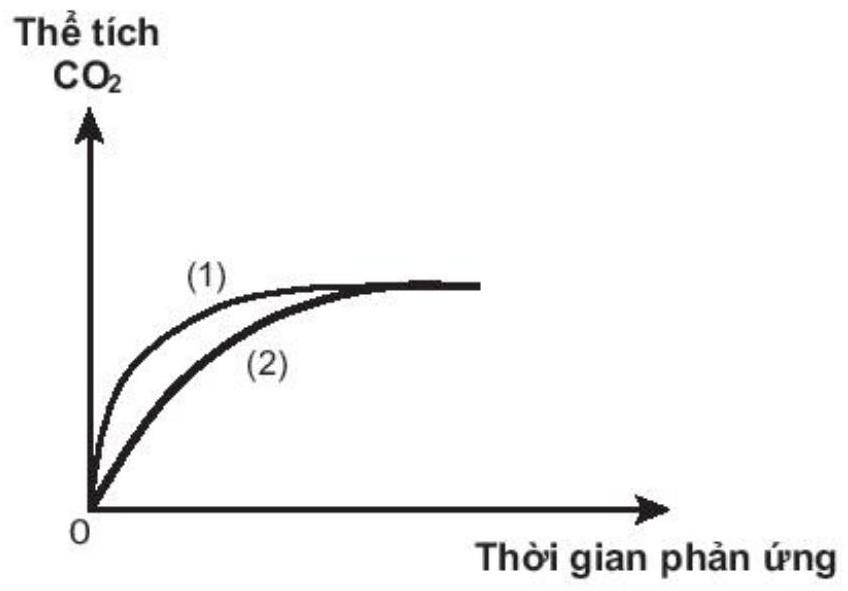
\includegraphics[max width=\textwidth, center]{2025_10_23_daab5c8457c85b365b9eg-53}

Phản ứng nào đã dùng HCl với nồng độ cao hơn?\\
19.17. Cho phản ứng hoá học sau:

$$
\mathrm{H}_{2} \mathrm{O}_{2} \rightarrow \mathrm{H}_{2} \mathrm{O}+\frac{1}{2} \mathrm{O}_{2}
$$

Biết rằng tốc độ của phản ứng này tuân theo biểu thức của định luật tác dụng khối lượng.\\
a) Hãy viết biểu thức tốc độ phản ứng.\\
b) Tốc độ phản ứng tức thời tăng dần hay giảm dần theo thời gian?\\
19.18. Cách nào sau đây sẽ làm củ khoai tây chín nhanh nhất?\\
A. Luộc trong nước sôi.\\
B. Hấp cách thuỷ trong nồi cơm.\\
C. Nướng ở $180^{\circ} \mathrm{C}$.\\
D. Hấp trên nồi hơi.\\
19.19. Các nhà khảo cổ thường tìm được xác các loài động thực vật thời tiền sử nguyên vẹn trong băng. Hãy giải thích tại sao băng lại giúp bảo quản xác động thực vật.\\
19.20. NOCl là chất khí độc, sinh ra do sự phân huỷ nước cường toan (hỗn hợp $\mathrm{HNO}_{3}$ và HCl có tỉ lệ mol $1: 3$ ). NOCl có tính oxi hoá mạnh, ở nhiệt độ cao bị phân huỷ theo phản ứng hoá học sau:

$$
2 \mathrm{NOCl} \rightarrow 2 \mathrm{NO}+\mathrm{Cl}_{2}
$$

Tốc độ phản ứng ở $70^{\circ} \mathrm{C}$ là $2.10^{-7} \mathrm{~mol} /(\mathrm{L} \cdot \mathrm{s})$ và ở $80^{\circ} \mathrm{C}$ là $4,5 \cdot 10^{-7} \mathrm{~mol} /(\mathrm{L} \cdot \mathrm{s})$.\\
a) Tính hệ số nhiệt độ $\gamma$ của phản ứng.\\
b) Dự đoán tốc độ phản ứng ở $60^{\circ} \mathrm{C}$.\\
19.21. Khi thắng đường để làm caramen hoặc nước hàng, ta thường dùng đường kính chứ không dùng đường phèn. Giải thích.\\
19.22. Khi dùng $\mathrm{MnO}_{2}$ làm xúc tác trong phản ứng phân huỷ $\mathrm{H}_{2} \mathrm{O}_{2}$, tại sao ta cần dùng $\mathrm{MnO}_{2}$ ở dạng bột chứ không dùng ở dạng viên.\\
19.23. Trong công nghiệp, vôi sông được sản xuất bằng cách nung đá vôi.

Phản ứng hoá học xảy ra như sau:

$$
\mathrm{CaCO}_{3} \rightarrow \mathrm{CaO}+\mathrm{CO}_{2}
$$

Khi nung, đá vôi cần phải được đập nhỏ nhưng không nên nghiền mịn đá vôi thành bột. Giải thích.

\section*{VẬN DỤNG}
19.24. Trong quá trình tổng hợp nitric acid, có giai đoạn đốt cháy $\mathrm{NH}_{3}$ bằng $\mathrm{O}_{2}$ có xúc tác. Phản ứng xảy ra trong pha khí như sau:

$$
4 \mathrm{NH}_{3}+5 \mathrm{O}_{2} \rightarrow 4 \mathrm{NO}+6 \mathrm{H}_{2} \mathrm{O}
$$

Trong một thí nghiệm, cho vào bình phản ứng (bình kín) 560 mL khí $\mathrm{NH}_{3}$ và 672 mL khí $\mathrm{O}_{2}$ (có xúc tác, các thể tích khí đo ở đktc). Sau khi thực hiện phản ứng 2,5 giờ, thấy có $0,432 \mathrm{~g}$ nước tạo thành.\\
a) Viết biểu thức tính tốc độ trung bình của phản ứng theo các chất tham gia và chất tạo thành trong phản ứng.\\
b) Tính tốc độ trung bình của phản ứng theo đơn vị $\mathrm{mol} / \mathrm{h}$.\\
c) Tính số $\mathrm{mol} \mathrm{NH}_{3}$ và $\mathrm{O}_{2}$ sau 2,5 giờ.\\
19.25. Thực hiện phản ứng sau: $\mathrm{CaCO}_{3}+2 \mathrm{HCl} \rightarrow \mathrm{CaCl}_{2}+\mathrm{CO}_{2} \uparrow+\mathrm{H}_{2} \mathrm{O}$

Theo dõi thể tích $\mathrm{CO}_{2}$ thoat ra theo thời gian, thu được đồ thị như sau (thể tích khí được đo ở áp suất khí quyển và nhiệt độ phòng).\\
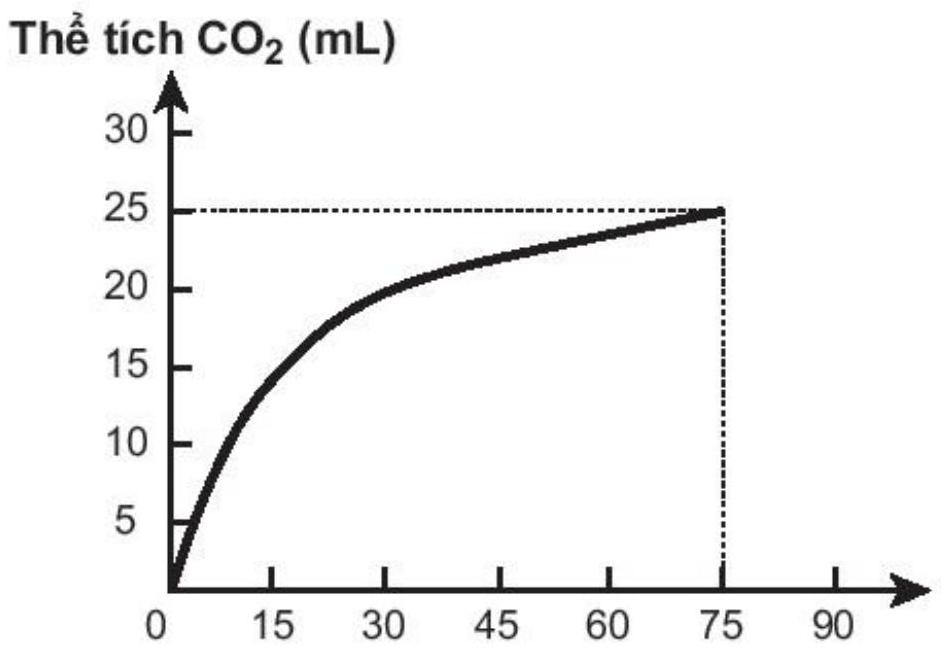
\includegraphics[max width=\textwidth, center]{2025_10_23_daab5c8457c85b365b9eg-54}

Trong các phát biểu sau, phát biểu nào không đúng?\\
A. Ở thời điểm 90 giây, tốc độ phản ứng bằng 0 .\\
B. Tốc độ phản ứng giảm dần theo thời gian.\\
C. Tốc độ trung bình của phản ứng trong khoảng thời gian từ thời điểm đầu đến 75 giây là $0,33 \mathrm{~mL} / \mathrm{s}$.\\
D. Tốc độ trung bình của phản ứng trong các khoảng thời gian 15 giây là như nhau\\
19.26. Thực hiện phản ứng sau:

$$
\mathrm{H}_{2} \mathrm{SO}_{4}+\mathrm{Na}_{2} \mathrm{~S}_{2} \mathrm{O}_{3} \rightarrow \mathrm{Na}_{2} \mathrm{SO}_{4}+\mathrm{SO}_{2}+\mathrm{S}+\mathrm{H}_{2} \mathrm{O}
$$

Theo dõi thể tích $\mathrm{SO}_{2}$ thoát ra theo thời gian, ta có bảng sau (thể tích khí được đo ở áp suất khí quyển và nhiệt độ phòng).

\begin{center}
\begin{tabular}{|c|c|c|c|c|c|c|c|c|}
\hline
Thòi gian (s) & 0 & 10 & 20 & 30 & 40 & 50 & 60 & 70 \\
\hline
Thể tích $\mathbf{S O}_{\mathbf{2}}(\mathbf{m L})$ & 0,0 & 12,5 & 20,0 & 26,5 & 31,0 & 32,5 & 33 & 33 \\
\hline
\end{tabular}
\end{center}

a) Vẽ đồ thị biểu diễn sự phụ thuộc thể tích khí $\mathrm{SO}_{2}$ vào thời gian phản ứng.\\
b) Thời điểm đầu, tốc độ phản ứng nhanh hay chậm?\\
c) Thời điểm kết thúc phản ứng, đồ thị có hình dạng như thế nào?\\
d) Tính tốc độ trung bình của phản ứng trong khoảng: từ $0 \div 10$ giây; từ $10 \div 20$ giây; từ $20 \div 40$ giây.\\
19.27. Xét phản ứng sau:

$$
2 \mathrm{ClO}_{2}+2 \mathrm{NaOH} \rightarrow \mathrm{NaClO}_{3}+\mathrm{NaClO}_{2}+\mathrm{H}_{2} \mathrm{O}
$$

Tốc độ phản ứng được viết như sau: $\mathrm{v}=\mathrm{k} \cdot \mathrm{C}_{\mathrm{ClO}_{2}}^{\mathrm{x}} \cdot \mathrm{C}_{\mathrm{NaOH}}^{\mathrm{y}}$\\
Thực hiện phản ứng với những nồng độ chất đầu khác nhau và đo tốc độ phản ứng tương ứng thu được kết quả trong bảng sau:

\begin{center}
\begin{tabular}{|c|c|c|c|}
\hline
STT & \begin{tabular}{c}
Nồng độ $\mathbf{C l O}_{\mathbf{2}}$ \\
$(\mathbf{M})$ \\
\end{tabular} & \begin{tabular}{c}
Nồng độ $\mathbf{N a O H}$ \\
$(\mathbf{M})$ \\
\end{tabular} & \begin{tabular}{c}
Tốc độ phản úng \\
$(\mathbf{m o l} /(\mathbf{L} . \mathbf{s}))$ \\
\end{tabular} \\
\hline
1 & 0,01 & 0,01 & $2.10^{-4}$ \\
\hline
2 & 0,02 & 0,01 & $8.10^{-4}$ \\
\hline
3 & 0,01 & 0,02 & $4.10^{-4}$ \\
\hline
\end{tabular}
\end{center}

Hãy tính x và y trong biểu thức tốc độ phản ứng.\\
19.28. Hãy đề xuất một phương pháp thực nghiệm để nghiên cứu tốc độ các phản ứng sau đây. Trong đó chỉ rõ: đại lượng nào em sẽ đo; đồ thị theo dõi sự thay đổi của đại lượng đó theo thời gian có dạng thế nào.\\
a) Phản ứng xảy ra trong dung dịch:

$$
\mathrm{CH}_{3} \mathrm{CH}_{2} \mathrm{Br}+\mathrm{H}_{2} \mathrm{O} \rightarrow \mathrm{CH}_{3} \mathrm{CH}_{2} \mathrm{OH}+\mathrm{HBr}
$$

b) Phản ứng xảy ra trong pha khí:

$$
2 \mathrm{NO}+\mathrm{Cl}_{2} \rightarrow 2 \mathrm{NOCl}
$$

19.29. Thực hiện phản ứng:

$$
2 \mathrm{ICl}+\mathrm{H}_{2} \rightarrow \mathrm{I}_{2}+2 \mathrm{HCl}
$$

Nồng độ đầu của ICl và $\mathrm{H}_{2}$ được lấy đúng theo tỉ lệ hợp thức. Nghiên cứu sự thay đổi nồng độ các chất tham gia và chất tạo thành trong phản ưng theo thời gian, thu được đồ thị sau:\\
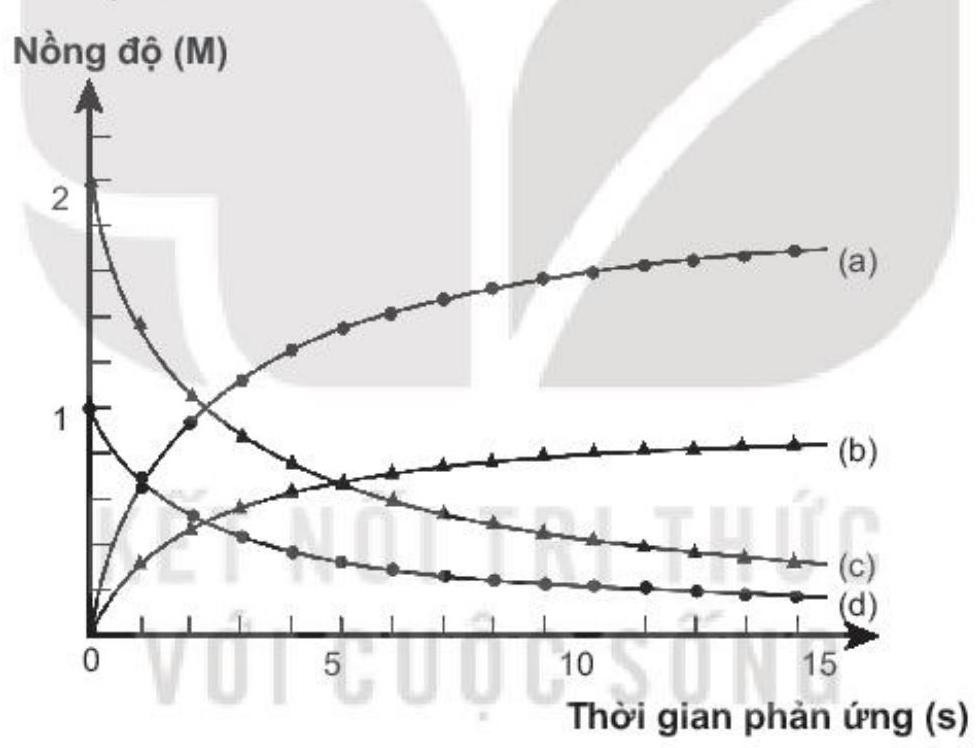
\includegraphics[max width=\textwidth, center]{2025_10_23_daab5c8457c85b365b9eg-56}

Cho biết các đường (a), (b), (c), (d) tương ứng với sự biến đổi nồng độ các chất nào trong phương trình phản ứng trên. Giải thích.\\
19.30. Phosgen ( $\mathrm{COCl}_{2}$ ) là một chất độc hoá học được sử dụng trong chiến tranh thế giới thứ nhất.\\
Phản ứng tổng hợp phosgen như sau: $\mathrm{CO}+\mathrm{Cl}_{2} \rightarrow \mathrm{COCl}_{2}$.\\
Biểu thức tốc độ phản ứng có dạng: $\mathrm{v}=\mathrm{k} \cdot \mathrm{C}_{\mathrm{CO}} \cdot \mathrm{C}_{\mathrm{Cl}_{2}}^{3 / 2}$.\\
Tốc độ phản ứng thay đổi như nào nếu:\\
a) Tăng nồng độ CO lên 2 lần.\\
b) Giảm nồng độ $\mathrm{Cl}_{2}$ xuống 4 lần.\\
19.31. Cho phản ứng hoá học sau:

$$
\mathrm{Zn}(\mathrm{~s})+\mathrm{H}_{2} \mathrm{SO}_{4}(\mathrm{aq}) \rightarrow \mathrm{ZnSO}_{4}(\mathrm{aq})+\mathrm{H}_{2}(\mathrm{~g})
$$

a) Ở nhiệt độ phòng, đo được sau 1 phút có $7,5 \mathrm{~mL}$ khí hydrogen thoát ra. Tính tốc độ trung bình của phản ứng theo hydrogen.\\
b) Ở nhiệt độ thấp, tốc độ phản ứng là $3 \mathrm{~mL} / \mathrm{min}$. Hãy tính xem sau bao lâu thì thu được $7,5 \mathrm{~mL}$ khí hydrogen.\\
19.32. Khi nhiệt độ phòng là $25^{\circ} \mathrm{C}$, cho 10 g đá vôi (dạng viên) vào cốc đựng 100 g dung dịch HCl loãng và nhanh chóng cho lên một cân điện tử. Đọc giá trị khối lượng cốc tại thời điểm ban đầu và sau 1 phút.\\
Lặp lại thí nghiệm khi nhiệt độ phòng là $35^{\circ} \mathrm{C}$. Kết quả thí nghiệm được ghi trong bảng sau:

\begin{center}
\begin{tabular}{|c|c|c|c|}
\hline
\multirow{2}{*}{STT} & \multirow{2}{*}{Nhiệt độ $\left({ }^{\circ} \mathrm{C}\right)$} & \multicolumn{2}{|c|}{Khối lượng cốc (g)} \\
\cline { 3 - 4 }
 &  & Thời điểm đầu & Sau 1 phút \\
\hline
1 & 25 & 235,40 & 235,13 \\
\hline
2 & 35 & 235,78 & 235,21 \\
\hline
\end{tabular}
\end{center}

a) Tính hệ số nhiệt độ của phản ứng.\\
b) Giả sử ban đầu cốc chứa dung dịch HCl và đá vôi có khối lượng $235,40 \mathrm{~g}$. Thực hiện thí nghiệm ở $45^{\circ} \mathrm{C}$. Hỏi sau 1 phút, khối lượng cốc là bao nhiêu? (Bỏ qua khối lượng nước bay hơi).\\
19.33. Có hai miếng iron có kích thước giống hệt nhau, một miếng là khối iron đặc (A), một miếng có nhiều lỗ nhỏ li ti bên trong và trên bề mặt (B). Thả hai miếng iron vào hai cốc đựng dung dịch HCl cùng thể tích và nồng độ, theo dõi thể tích khí hydrogen thoát ra theo thời gian. Vẽ đồ thị thể tích khí theo thời gian, thu được hai đồ thị sau:\\
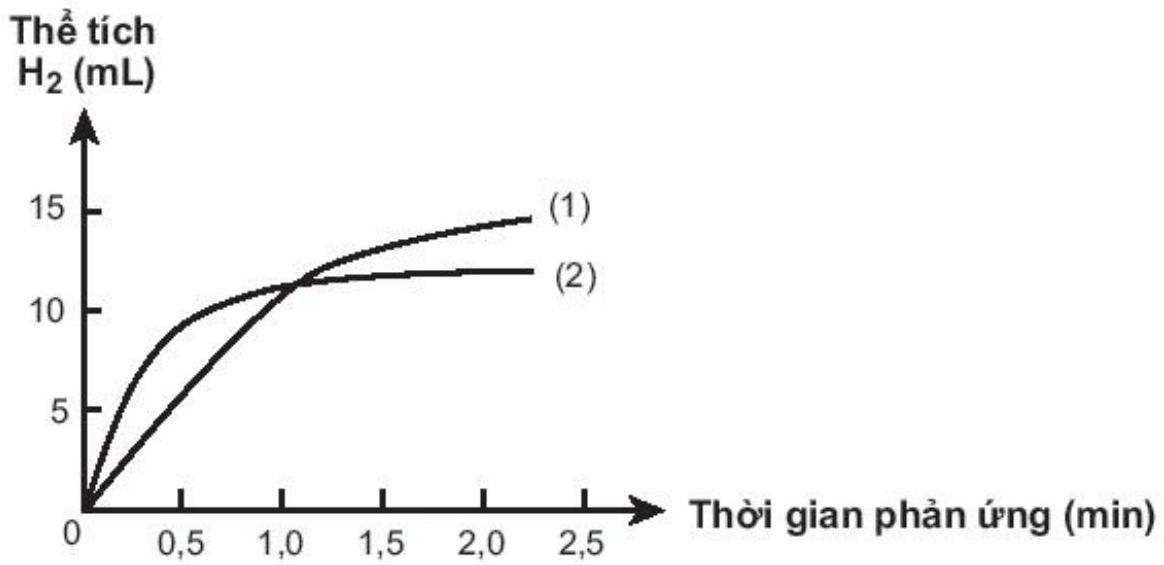
\includegraphics[max width=\textwidth, center]{2025_10_23_daab5c8457c85b365b9eg-58}

Cho biết đồ thị nào mô tả tốc độ thoát khí từ miếng sắt A , miếng sắt B . Giải thích.\\
19.34. Xúc tác có hiệu quả cao là xúc tác làm tăng nhanh tốc độ phản ứng. Hai chất $\mathrm{MnO}_{2}$ và $\mathrm{Fe}_{2} \mathrm{O}_{3}$ đều có khả năng xúc tác cho phản ứng phân huỷ $\mathrm{H}_{2} \mathrm{O}_{2}$. Đo nồng độ $\mathrm{H}_{2} \mathrm{O}_{2}$ theo thời gian, thu được đồ thị sau:\\
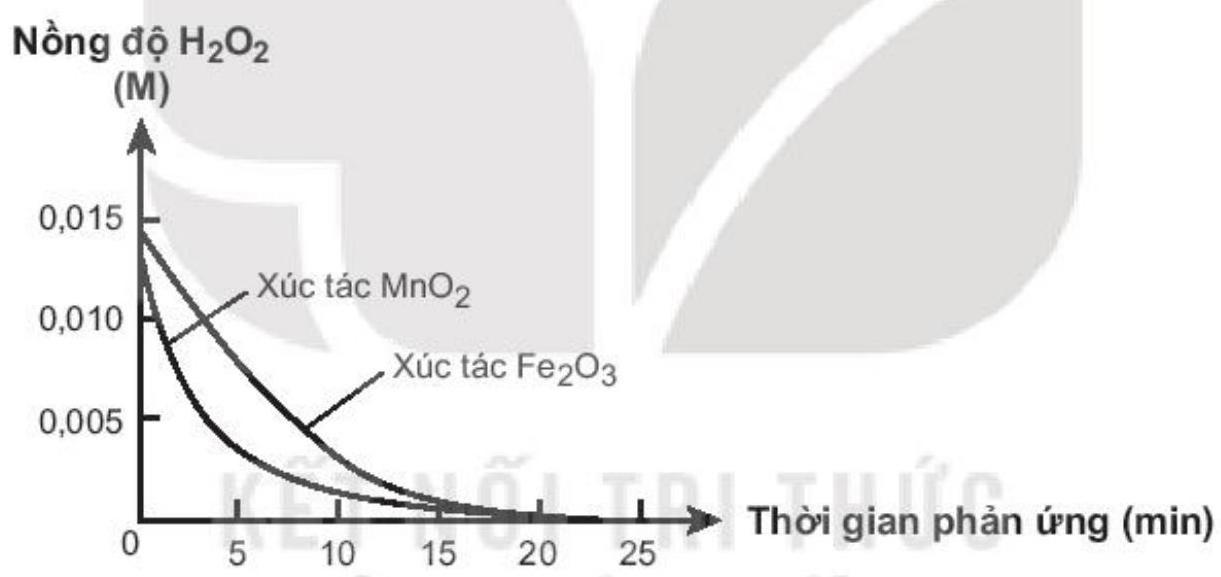
\includegraphics[max width=\textwidth, center]{2025_10_23_daab5c8457c85b365b9eg-58(1)}

Cho biết xúc tác nào có hiệu quả hơn. Giải thích.\\
19.35. Khí oxygen và hydrogen có thể cùng tồn tại trong một bình kín ở điều kiện bình thường mà không nguy hiểm. Nhưng khi có tia lửa điện hoặc một it bột kim loại được thêm vào bình thì lập tức có phản ứng mãnh liệt xảy ra và có thể gây nổ.\\
a) Tia lửa điện có phải chất xúc tác không? Giải thích.\\
b) Bột kim loại có phải chất xúc tác không? Giải thích.

\section*{Bài 20. ÔN TẬP CHUƠNG 6}
\section*{NHẬN BIẾT}
20.1. Cho phản ứng hoá học sau:

$$
\mathrm{C}(\mathrm{~s})+\mathrm{O}_{2}(\mathrm{~g}) \rightarrow \mathrm{CO}_{2}(\mathrm{~g})
$$

Yếu tố nào sau đây không ảnh hưởng đến tốc độ phản ứng trên?\\
A. Nhiệt độ.\\
B. Áp suất $\mathrm{O}_{2}$.\\
C. Hàm lượng carbon.\\
D. Diện tích bề mặt carbon.\\
20.2. Cho Zn phản ứng với HCl để điều chế hydrogen. Hãy nêu 3 cách để làm tăng tốc độ phản ứng này.\\
20.3. Khí oxygen được điều chế trong phòng thí nghiệm bằng cách nhiệt phân potassium chlorate. Để thí nghiệm thành công và rút ngắn thời gian tiến hành có thể dùng một số biện pháp sau:\\
(1) Dùng chất xúc tác manganese dioxide.\\
(2) Nung ở nhiệt độ cao.\\
(3) Dùng phương pháp dời nước để thu khí oxygen.\\
(4) Đập nhỏ potassium chlorate.\\
(5) Trộn đều bột potassium chlorate và xúc tác.

Số biện pháp dùng để tăng tốc độ phản ưng là\\
A. 2 .\\
B. 3 .\\
C. 4 .\\
D. 5 .\\
20.4. Phát biểu nào sau đây không đúng?\\
A. Nhiên liệu cháy ở trên vùng cao nhanh hơn khi cháy ở vùng thấp.\\
B. Thực phẩm được bảo quản ở nhiệt độ thấp hơn sẽ giữ được lâu hơn.\\
C. Dừng men làm chất xúc tác để chuyển hoá cơm nếp thành rượu.\\
D. Nếu không cho nước dưa chua khi muối dưa thì dưa vẫn sẽ chua nhưng chậm hơn.\\
20.5. Trong quy trình sản xuất sulfuric acid, xảy ra phản ứng hoá học sau:

$$
2 \mathrm{SO}_{2}+\mathrm{O}_{2} \xrightarrow{\mathrm{~V}_{2} \mathrm{O}_{5}} 2 \mathrm{SO}_{3}
$$

Phát biểu nào sau đây không đúng?\\
A. Khi tăng áp suất khí $\mathrm{SO}_{2}$ hay $\mathrm{O}_{2}$ thì tốc độ phản ứng đều tăng lên.\\
B. Tăng diện tích bề mặt của xúc tác $\mathrm{V}_{2} \mathrm{O}_{5}$ sẽ làm tăng tốc độ phản ứng.\\
C. Xúc tác sẽ dần chuyển hoá thành chất khác nhưng khối lượng không đổi.\\
D. Cần làm nóng bình phản ứng để đẩy nhanh tốc độ phản ứng.

\section*{THÔNG HIỂU}
20.6. Khi để ở nhiệt độ $30^{\circ} \mathrm{C}$, một quả táo bị hư sau 3 ngày. Khi được bảo quản ở $0^{\circ} \mathrm{C}$ (trong tủ lạnh), quả táo đó bị hư sau 24 ngày.\\
a) Hãy tính hệ số nhiệt độ của phản ứng xảy ra khi quả táo bị hư.\\
b) Nếu bảo quản ở $20^{\circ} \mathrm{C}$, quả táo sẽ bị hư sau bao nhiêu ngày?\\
20.7. Cho biết những phát biểu sau đây là đúng hay sai. Giải thích.\\
(1) Để phản ứng hoá học xảy ra, các hạt (phân tử, nguyên tử, ion) của chất phản ứng phải va chạm với nhau.\\
(2) Khi áp suất khí CO tăng, tốc độ phản ứng $4 \mathrm{CO}+\mathrm{Fe}_{3} \mathrm{O}_{4} \rightarrow 4 \mathrm{CO}_{2}+3 \mathrm{Fe}$ tăng lên.\\
(3) Khi tăng nhiệt độ lên $10^{\circ} \mathrm{C}$, tốc độ của các phản ứng hoá học đều tăng gấp đôi.\\
(4) Nếu năng lượng va chạm giữa hai phân tử chất phản ứng nhỏ hơn năng lượng hoạt hoá thì sẽ gây ra phản ứng hoá học.\\
(5) Phản ứng có năng lượng hoạt hoá càng thấp thì xảy ra càng nhanh.\\
20.8. Ở $225^{\circ} \mathrm{C}$, khí $\mathrm{NO}_{2}$ và $\mathrm{O}_{2}$ có phản ứng sau:

$$
2 \mathrm{NO}+\mathrm{O}_{2} \rightarrow 2 \mathrm{NO}_{2}
$$

Biểu thức tốc độ phản ứng có dạng: $\mathrm{v}=\mathrm{k} \cdot \mathrm{C}_{\mathrm{NO}}^{2} \cdot \mathrm{C}_{\mathrm{O}_{2}}$.\\
Cho biết tốc độ phản ứng sẽ thay đổi như thế nào nếu:\\
(i) Tăng nồng độ NO lên 2 lần.\\
(ii) Giảm nồng độ $\mathrm{O}_{2}$ đi 3 lần.\\
(iii) Tăng nồng độ $\mathrm{NO}_{2}$ lên 2 lần.

\section*{VẬN DỤNG}
20.9. Phản ứng phân huỷ ethyl iodide trong pha khí xảy ra như sau:

$$
\mathrm{C}_{2} \mathrm{H}_{5} \mathrm{I} \rightarrow \mathrm{C}_{2} \mathrm{H}_{4}+\mathrm{HI}
$$

Ở $127^{\circ} \mathrm{C}$, hằng số tốc độ của phản ứng là $1,60 \cdot 10^{-7} \mathrm{~s}^{-1}$, ở $227^{\circ} \mathrm{C}$ là $4,25 \cdot 10^{-4} \mathrm{~s}^{-1}$.\\
a) Hãy tính hệ số nhiệt độ của phản ứng trên.\\
b) Tính hằng số tốc độ của phản ứng ở $167^{\circ} \mathrm{C}$.\\
20.10. Ở vùng đồng bằng (độ cao gần mực nước biển), nước sôi ở $100^{\circ} \mathrm{C}$. Trên đỉnh núi Fansipan (cao 3200 m so với mực nước biển), nước sôi ở $90^{\circ} \mathrm{C}$. Khi luộc chín một miếng thịt trong nước sôi, ở vùng đồng bằng mất 3,2 phút, trong khi đó trên đỉnh Fansipan mất 3,8 phút.\\
a) Tính hệ số nhiệt độ của phản ứng làm chín miếng thịt trên.\\
b) Nếu luộc miếng thịt trên đỉnh núi cao hơn, tại đó nước sôi ở $80^{\circ} \mathrm{C}$ thì mất bao lâu để luộc chín miếng thịt?\\
20.11. Chất độc màu da cam dioxin gây tác hại vô cùng nghiêm trọng đối với môi trường và sức khoẻ con người. Nó phân huỷ vô cùng chậm trong đất. Nghiên cứu cho thấy phải mất tám năm để lượng dioxin trong đất giảm đi một nửa. Nếu một mảnh đất có chứa $0,128 \mathrm{mg}$ dioxin thì sau bao lâu lượng dioxin còn lại là $10^{-6} \mathrm{~g}$ dioxin.\\
20.12. Phản ứng phân huỷ một loại hoạt chất kháng sinh có hệ số nhiệt độ là 2,5 . Ở $27^{\circ} \mathrm{C}$, sau 10 giờ thì lượng hoạt chất giảm đi một nửa.\\
a) Khi đưa vào cơ thể người ( $37^{\circ} \mathrm{C}$ ) thì lượng hoạt chất giảm đi một nửa sau bao lâu?\\
b) Sau bao lâu thì hoạt chất kháng sinh này trong cơ thể người còn lại $12,5 \%$ so với ban đầu?

\section*{Bài 21. NHÓM HALOGEN}
\section*{NHẬN BIÉT}
21.1. Số electron ở lớp ngoài cùng của mỗi nguyên tử nguyên tố halogen là\\
A. 5 .\\
B. 7 .\\
C. 2 .\\
D. 8 .\\
21.2. Tính chất hoá học đặc trưng của các đơn chất halogen là\\
A. tính khử.\\
B. tính base.\\
C. tính acid.\\
D. tính oxi hoá.\\
21.3. Trong tự nhiên, nguyên tố fluorine tồn tại phổ biến nhất ở dạng hợp chất là\\
A. $\mathrm{Na}_{3} \mathrm{AlF}_{6}$.\\
B. NaF .\\
C. HF .\\
D. $\mathrm{CaF}_{2}$.\\
21.4. Ở điều kiện thường, halogen tồn tại ở thể rắn, có màu đen tím là\\
A. $F_{2}$.\\
B. $\mathrm{Br}_{2}$.\\
C. $\mathrm{I}_{2}$.\\
D. $\mathrm{Cl}_{2}$.\\
21.5. Muối nào có nhiều nhất trong nước biển với nồng độ khoảng $3 \%$ ?\\
A. NaCl .\\
B. KCl .\\
C. $\mathrm{MgCl}_{2}$.\\
D. NaF .\\
21.6. Số oxi hoá cao nhất mà nguyên tử chlorine thể hiện được trong các hợp chất là\\
A. -1 .\\
B. +7 .\\
C. +5 .\\
D. +1 .\\
21.7. Các nguyên tố halogen thuộc nhóm nào trong bảng tuần hoàn?\\
A. VIIIA.\\
B. VIA.\\
C. VIIA.\\
D. IIA.\\
21.8. Trong nhóm halogen, đơn chất có tính oxi hoá mạnh nhất là\\
A. $F_{2}$.\\
B. $\mathrm{Cl}_{2}$.\\
C. $\mathrm{Br}_{2}$.\\
D. $\mathrm{I}_{2}$.\\
21.9. Khi đun nóng, chất thăng hoa chuyển từ thể rắn sang thể hơi màu tím là\\
A. $F_{2}$.\\
B. $\mathrm{Cl}_{2}$.\\
C. $\mathrm{Br}_{2}$.\\
D. $\mathrm{I}_{2}$.\\
21.10. Halogen nào sau đây được dùng để khử trùng nước sinh hoạt?\\
A. $F_{2}$.\\
B. $\mathrm{Cl}_{2}$.\\
C. $\mathrm{Br}_{2}$.\\
D. $\mathrm{I}_{2}$.\\
21.11. Trong cơ thể người, nguyên tố iodine tập trung ở tuyến nào sau đây?\\
A. Tuyến thượng thận.\\
B. Tuyến tuy.\\
C. Tuyến yên.\\
D. Tuyến giáp trạng.\\
21.12. Trong dãy halogen, nguyên tử có độ âm điện nhỏ nhất là\\
A. fluorine.\\
B. chlorine.\\
C. bromine.\\
D. iodine.

\section*{THÔNG HIỂU}
21.13. Trong nhóm halogen, từ fluorine đến iodine, bán kính nguyên tử biến đổi như thế nào?\\
A. Giảm dần.\\
B. Không đổi.\\
C. Tăng dần.\\
D. Tuần hoàn.\\
21.14. Trong nhóm halogen, nguyên tử nguyên tố thể hiện khuynh hướng nhận 1 electron yếu nhất là\\
A. fluorine.\\
B. chlorine.\\
C. bromine.\\
D. iodine.\\
21.15. Trong nhóm halogen, từ fluorine đến iodine, nhiệt độ nóng chảy biến đổi như thế nào?\\
A. Giảm dần.\\
B. Tăng dần.\\
C. Không đổi.\\
D. Tuần hoàn.\\
21.16. Halogen phản ứng mãnh liệt với hydrogen ngay cả trong bóng tối là\\
A. $F_{2}$.\\
B. $\mathrm{Cl}_{2}$.\\
C. $\mathrm{Br}_{2}$.\\
D. $\mathrm{I}_{2}$.\\
21.17. Khi tác dụng với kim loại, các nguyên tử halogen thể hiện xu hướng nào sau đây?\\
A. Nhường 1 electron.\\
B. Nhận 1 electron.\\
C. Nhường 7 electron.\\
D. Góp chung 1 electron.\\
21.18. Hít thở không khí có chứa khí nào sau đây vượt ngưỡng $30 \mu \mathrm{~g} / \mathrm{m}^{3}$ không khí (QCVN 06:2009/BTNMT) sẽ tiềm ẩn nguy cơ gây viêm đường hô hấp, co thắt phế quản, khó thở?\\
A. $\mathrm{O}_{2}$.\\
B. $\mathrm{Cl}_{2}$.\\
C. $\mathrm{N}_{2}$.\\
D. $\mathrm{O}_{3}$.\\
21.19. Quá trình sản xuất khí chlorine trong công nghiệp hiện nay dựa trên phản ứng nào sau đây?\\
A. $\mathrm{MnO}_{2}+4 \mathrm{HCl} \xrightarrow{\mathrm{t}^{\circ}} \mathrm{MnCl}_{2}+\mathrm{Cl}_{2}+2 \mathrm{H}_{2} \mathrm{O}$.\\
B. $\mathrm{Cl}_{2}+2 \mathrm{NaBr} \longrightarrow 2 \mathrm{NaCl}+\mathrm{Br}_{2}$.\\
C. $2 \mathrm{NaCl}+2 \mathrm{H}_{2} \mathrm{O} \xrightarrow[\text { mn }]{\text { dpdd }} 2 \mathrm{NaOH}+\mathrm{Cl}_{2}+\mathrm{H}_{2}$.\\
D. $2 \mathrm{NaOH}+\mathrm{Cl}_{2} \longrightarrow \mathrm{NaCl}+\mathrm{NaClO}+\mathrm{H}_{2} \mathrm{O}$.\\
21.20. Chỉ thị nào sau đây thường dùng để nhận biết dung dịch $\mathrm{I}_{2}$ ?\\
A. Phenolphtalein.\\
B. Hồ tinh bột.\\
C. Quỳ tím.\\
D. Nước vôi trong.

\section*{VÂN DỤNG}
21.21. Thực nghiệm cho thấy các phản ứng: $\mathrm{H}_{2}(\mathrm{~g})+\mathrm{X}_{2}(\mathrm{~g}) \longrightarrow 2 \mathrm{HX}(\mathrm{g})$ trong dãy halogen xảy ra với mức độ giảm dần từ $\mathrm{F}_{2}$ đến $\mathrm{I}_{2}$.\\
Biến thiên enthalpy của các phản ứng thay đổi như thế nào trong dãy trên?\\
21.22. Đốt cháy hoàn toàn $0,48 \mathrm{~g}$ kim loại M (hoá trị II) bằng khí chlorine, thu được $1,332 \mathrm{~g}$ muối chloride. Xác định kim loại M .\\
21.23. Nung nóng một bình bằng thép có chứa $0,04 \mathrm{~mol} \mathrm{H}_{2}$ và $0,04 \mathrm{~mol} \mathrm{Cl}_{2}$ để thực hiện phản ứng, thu được $0,072 \mathrm{~mol}$ khí HCl .\\
a) Tính hiệu suất của phản ứng tạo thành HCl .\\
b) Ở cùng nhiệt độ thường, áp suất suất khí trong bình trước và sau phản ứng lần lượt là $P_{1}$ và $P_{2}$. Hãy so sánh $P_{1}$ và $P_{2}$.\\
21.24. Có hai ống nghiệm, mỗi ống chứa 2 mL dung dịch muối X của kali. Cho vài giọt dung dịch $\mathrm{AgNO}_{3}$ vào ống thứ nhất, thu được kết tủa màu vàng. Nhỏ vài giọt nước $\mathrm{Br}_{2}$ vào ống thứ hai, lắc đều rồi thêm hồ tinh bột, thấy có màu xanh tím. Xác định công thức hoá học của X và viết phương trình hoá học của các phản ứng.\\
21.25. Trong phòng thí nghiệm, khí chlorine được điều chế, làm khô và thu vào bình theo sơ đồ dưới đây.\\
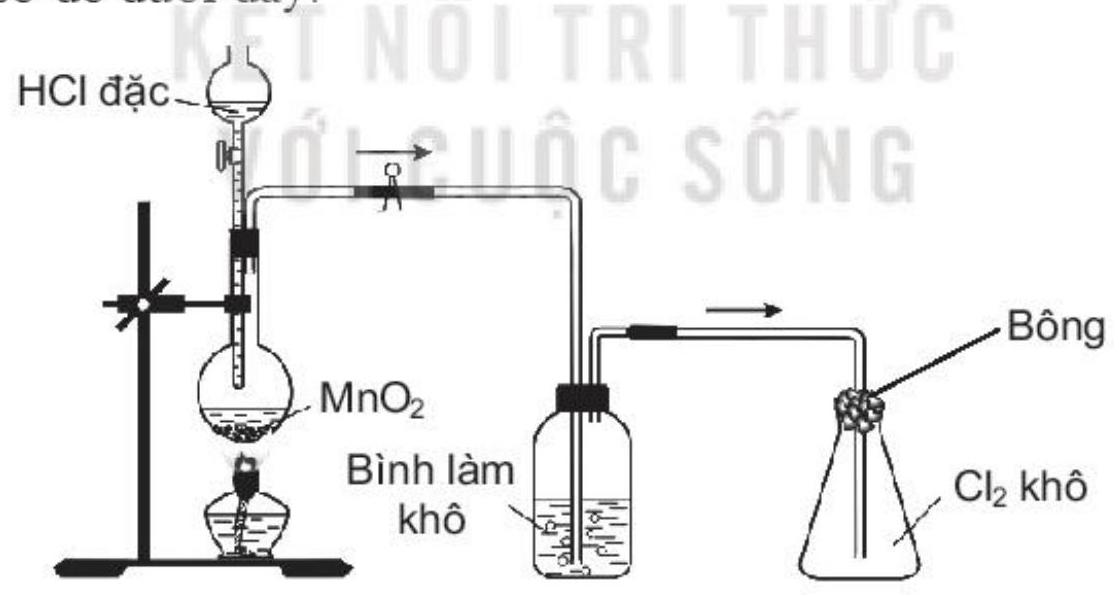
\includegraphics[max width=\textwidth, center]{2025_10_23_daab5c8457c85b365b9eg-64}

Hãy đề xuất một dung dịch để sử dụng cho từng mục đích sau:\\
a) Cho vào bình làm khô để làm khô khí $\mathrm{Cl}_{2}$.\\
b) Tẩm vào bông đậy bình thu khí để hạn chế khí $\mathrm{Cl}_{2}$ bay ra. Giải thích và viết phương trình hoá học minh hoạ nếu có.

\section*{Bài 22. HYDROGEN HALIDE. MUỐI HALIDE}
\section*{NHẬN BIẾT}
22.1. Ở trạng thái lỏng, giữa các phân tử hydrogen halide nào sau đây tạo được liên kết hydrogen mạnh?\\
A. HCl .\\
B. HI .\\
C. HF .\\
D. HBr .\\
22.2. Hydrogen halide nào sau đây có nhiệt độ sôi cao nhất ở áp suất thường?\\
A. HCl .\\
B. HBr .\\
C. HF .\\
D. HI .\\
22.3. Trong dãy hydrogen halide, từ HF đến HI , độ bền liên kết biến đổi như thế nào?\\
A. Tăng dần.\\
B. Giảm dần.\\
C. Không đổi.\\
D. Tuần hoàn.\\
22.4. Dung dịch hydrohalic acid nào sau đây có tính acid yếu?\\
A. HF .\\
B. HBr .\\
C. HCl .\\
D. HI .\\
22.5. Nhỏ vài giọt dung dịch nào sau đây vào dung dịch $\mathrm{AgNO}_{3}$ thu được kết tủa màu vàng nhạt?\\
A. HCl .\\
B. NaBr .\\
C. NaCl .\\
D. HF .\\
22.6. Trong điều kiện không có không khí, đinh sắt tác dụng với dung dịch HCl thu được các sản phẩm là\\
A. $\mathrm{FeCl}_{3}$ và $\mathrm{H}_{2}$.\\
B. $\mathrm{FeCl}_{2}$ và $\mathrm{Cl}_{2}$.\\
C. $\mathrm{FeCl}_{3}$ và $\mathrm{Cl}_{2}$.\\
D. $\mathrm{FeCl}_{2}$ và $\mathrm{H}_{2}$.\\
22.7. Hydrohalic acid thường được dùng để đánh sạch bề mặt kim loại trước khi sơn, hàn, mạ điện là\\
A. HBr .\\
B. HF .\\
C. HI.\\
D. HCl .\\
22.8. Hydrohalic acid được dùng làm nguyên liệu để sản xuất hợp chất chống dính teflon là\\
A. HF .\\
B. HCl .\\
C. HBr .\\
D. HI.\\
22.9. Dung dịch nào sau đây có thể phân biệt được các ion $\mathrm{F}^{-}, \mathrm{Cl}^{-}, \mathrm{Br}^{-}, \mathrm{I}^{-}$ trong dung dịch muối?\\
A. NaOH .\\
B. HCl .\\
C. $\mathrm{AgNO}_{3}$.\\
D. $\mathrm{KNO}_{3}$.\\
22.10. KBr thể hiện tính khử khi đun nóng với dung dịch nào sau đây?\\
A. $\mathrm{AgNO}_{3}$.\\
B. $\mathrm{H}_{2} \mathrm{SO}_{4}$ đặc.\\
C. HCl .\\
D. $\mathrm{H}_{2} \mathrm{SO}_{4}$ loãng.

\section*{THÔNG HIỂU}
22.11. Trong dãy hydrogen halide, từ HCl đến HI , nhiệt độ sôi tăng dần chủ yếu do nguyên nhân nào sau đây?\\
A. Tương tác van der Waals tăng dần.\\
B. Phân tử khối tăng dần.\\
C. Độ bền liên kết giảm dần.\\
D. Độ phân cực liên kết giảm dần.\\
22.12. Trong dãy hydrogen halide, từ HF đến HI , độ phân cực của liên kết biến đổi như thế nào?\\
A. Tuần hoàn.\\
B. Tăng dần.\\
C. Giảm dần.\\
D. Không đổi.\\
22.13. Hydrochloric acid đặc thể hiện tính khử khi tác dụng với chất nào sau đây?\\
A. $\mathrm{NaHCO}_{3}$.\\
B. $\mathrm{CaCO}_{3}$.\\
C. NaOH .\\
D. $\mathrm{MnO}_{2}$.\\
22.14. Hydrochloric acid loãng thể hiện tính oxi hoá khi tác dụng với chất nào sau đây?\\
A. $\mathrm{FeCO}_{3}$.\\
B. Fe.\\
C. $\mathrm{Fe}(\mathrm{OH})_{2}$.\\
D. $\mathrm{Fe}_{2} \mathrm{O}_{3}$.\\
22.15. Thuốc thử nào sau đây phân biệt được hai dung dịch HCl và NaCl ?\\
A. Phenolphthalein.\\
B. Hồ tinh bột.\\
C. Quỳ tím.\\
D. Nước brom.\\
22.16. Dung dịch HF có khả năng ăn mòn thuỷ tinh là do xảy ra phản ứng hoá học nào sau đây?\\
A. $\mathrm{SiO}_{2}+4 \mathrm{HF} \longrightarrow \mathrm{SiF}_{4}+2 \mathrm{H}_{2} \mathrm{O}$.\\
B. $\mathrm{NaOH}+\mathrm{HF} \longrightarrow \mathrm{NaF}+\mathrm{H}_{2} \mathrm{O}$.\\
C. $\mathrm{H}_{2}+\mathrm{F}_{2} \longrightarrow 2 \mathrm{HF}$.\\
D. $2 \mathrm{~F}_{2}+2 \mathrm{H}_{2} \mathrm{O} \longrightarrow 4 \mathrm{HF}+\mathrm{O}_{2}$.\\
22.17. Trong dãy hydrohalic acid, từ HF đến HI , tính acid tăng dần do nguyên nhân chính là\\
A. tương tác van der Waals tăng dần.\\
B. độ phân cực liên kết giảm dần.\\
C. phân tử khối tăng dần.\\
D. độ bền liên kết giảm dần.\\
22.18. Cho muối halide nào sau đây tác dụng với dung dịch $\mathrm{H}_{2} \mathrm{SO}_{4}$ đặc, nóng thì chỉ xảy ra phản ứng trao đổi?\\
A. KBr .\\
B. KI .\\
C. NaCl .\\
D. NaBr .\\
22.19. Phát biểu nào sau đây không đúng?\\
A. Dung dịch hydrofluoric acid có khả năng ăn mòn thuỷ tinh.\\
B. NaCl rắn tác dụng với $\mathrm{H}_{2} \mathrm{SO}_{4}$ đặc, nóng, thu được hydrogen chloride.\\
C. Hydrogen chloride tan nhiều trong nước.\\
D. Lực acid trong dãy hydrohalic acid giảm dần từ HF đến HI .\\
22.20. Dung dịch nào sau đây có thể phân biệt hai dung dịch NaF và NaCl ?\\
A. HCl .\\
B. HF .\\
C. $\mathrm{AgNO}_{3}$.\\
D. $\mathrm{Br}_{2}$

\section*{VẬN DỤNG}
22.21. Thực hiện thí nghiệm thử tính tan của hydrogen chloride theo các bước sau:\\
Bước 1: chuẩn bị một bình khô chứa khí HCl , đậy bình bằng nút cao su có ống thuỷ tinh xuyên qua và một cốc nước.\\
Bước 2: nhúng ống thuỷ tinh vào cốc nước, thấy\\
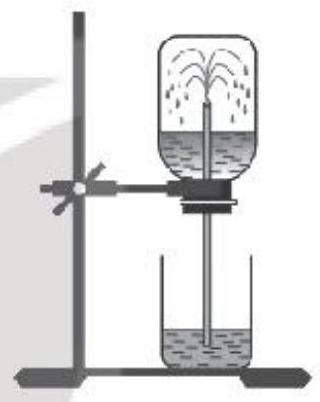
\includegraphics[max width=\textwidth, center]{2025_10_23_daab5c8457c85b365b9eg-67}

Thí nghiệm về tính tan của khi HCl .\\
nước phun vào bình (xem hình bên).\\
a) Hiện tượng nước phun vào bình cho thấy áp suất khí HCl trong bình đã tăng hay giảm rất nhanh. Giải thích.\\
b) Sự biến đổi áp suất như vậy đã chưng tỏ tính chất gì của khí HCl ?\\
22.22. Trong cơ thể người, dịch vị dạ dày có môi trường acid $(\mathrm{HCl}), \mathrm{pH}=1,6 \div 2,4$ giúp hỗ trợ tiêu hoá.\\
a) Một bệnh nhân bị đau đạ dày do dư thừa acid được kê đơn thuốc uống có chứa $\mathrm{NaHCO}_{3}$. Viết phản ứng minh hoạ tác dụng của thuốc.\\
b) Ở $37^{\circ} \mathrm{C}$, tinh bột bị thuỷ phân thành glucose trong môi trường acid $(\mathrm{HCl})$ có xúc tác enzyme. Viết phương trình hoá học của phản ứng xảy ra.\\
22.23. Có hai ống nghiệm, mỗi ống chứa 2 mL dung dịch muối của sodium.

Cho vài giọt dung dịch $\mathrm{AgNO}_{3}$ vào ống thứ nhất, thu được kết tủa màu vàng nhạt. Nhỏ vài giọt nước $\mathrm{Cl}_{2}$ vào ống thứ hai, lắc nhẹ, thêm 1 mL benzene và\\
lắc đều, thấy benzene từ không màu chuyển sang màu da cam. Xác định công thức của muối sodium và viết phương trình hoá học của các phản ứng xảy ra.\\
22.24. Cho các dung dịch hydrochloric acid, sodium chloride, iodine, kí hiệu ngẫu nhiên là $\mathrm{X}, \mathrm{Y}, \mathrm{Z}$.

Một số kết quả thí nghiệm được ghi lại ở bảng sau.

\begin{center}
\begin{tabular}{|c|c|c|}
\hline
Chất thử & Thuốc thử & Hiện tượng \\
\hline
X & Hồ tinh bột & Xuất hiện màu xanh tím \\
\hline
Z & Baking soda, $\mathrm{NaHCO}_{3}$ & Có bọt khí bay ra \\
\hline
\end{tabular}
\end{center}

Các dung dịch ban đầu được kí hiệu tương ứng là\\
A. $Z, Y, X$.\\
B. $Y, X, Z$.\\
C. $Y, Z, X$.\\
D. $X, Z, Y$.

\section*{Bài 23. ÔN TẬP CHƯƠNG 7}
\section*{NHẬN BIẾT}
23.1. Nguyên tử halogen nào sau đây chỉ thể hiện số oxi hoá -1 trong các hợp chất?\\
A. Fluorine.\\
B. Chlorine.\\
C. Bromine.\\
D. Iodine.\\
23.2. Trong y học, halogen nào sau đây được hoà tan trong cồn để dùng làm thuốc sát trùng ngoài da?\\
A. Fluorine.\\
B. Chlorine.\\
C. Iodine.\\
D. Bromine.\\
23.3. Trong tự nhiên, nguyên tố chlorine tồn tại phổ biến nhất ở dạng hợp chất nào sau đây?\\
A. $\mathrm{MgCl}_{2}$.\\
B. NaCl .\\
C. KCl .\\
D. HCl .\\
23.4. Cấu hình electron lớp ngoài cùng của nguyên tử các nguyên tố halogen có dạng chung là\\
A. $n s^{2} n p^{5}$.\\
B. $\mathrm{ns}^{2}$.\\
C. $\mathrm{ns}^{2} \mathrm{np}^{6}$.\\
D. $n s^{2} n p^{4}$.\\
23.5. Ở điều kiện thường, halogen nào sau đây tồn tại ở thể lỏng, có màu nâu đỏ, gây bỏng sâu nếu rơi vào da?\\
A. $F_{2}$.\\
B. $\mathrm{Cl}_{2}$.\\
C. $\mathrm{I}_{2}$.\\
D. $\mathrm{Br}_{2}$.\\
23.6. Trong dãy hydrogen halide, từ HF đến HI , độ dài liên kết biến đổi như thế nào?\\
A. Không đổi.\\
B. Giảm dần.\\
C. Tăng dần.\\
D. Tuần hoàn.\\
23.7. Dung dịch hydrohalic acid có khả năng ăn mòn thuỷ tinh là\\
A. HCl .\\
B. HI .\\
C. HF .\\
D. HBr .\\
23.8. Trong phòng thí nghiệm, có thể điều chế khí $\mathrm{Cl}_{2}$ khi cho chất rắn nào sau đây tác dụng với dung dịch HCl đặc, đun nóng?\\
A. $\mathrm{CaCO}_{3}$.\\
B. $\mathrm{NaHCO}_{3}$.\\
C. FeO .\\
D. $\mathrm{MnO}_{2}$.\\
23.9. Cho khí $\mathrm{Cl}_{2}$ tác dụng với dung dịch KOH , đun nóng, thu được dung dịch chứa muối KCl và muối nào sau đây?\\
A. KClO .\\
B. $\mathrm{KClO}_{3}$.\\
C. $\mathrm{KClO}_{4}$.\\
D. $\mathrm{KClO}_{2}$.

\section*{THÔNG HIỂU}
23.10. Hydrohalic acid nào sau đây có tính acid mạnh nhất?\\
A. HI.\\
B. HF .\\
C. HCl .\\
D. HBr .\\
23.11. Quặng apatite, loại quặng phổ biến trong tự nhiên có chứa nguyên tố fluorine, có thành phần hoá học chính là\\
A. $\mathrm{CF}_{3} \mathrm{Cl}$.\\
B. NaF .\\
C. $\mathrm{Na}_{3} \mathrm{AlF}_{6}$\\
D. $\mathrm{Ca}_{10}\left(\mathrm{PO}_{4}\right)_{6} \mathrm{~F}_{2}$.\\
23.12. Ở nhiệt độ cao và có xúc tác, phản ứng giữa hydrogen với halogen nào sau đây xảy ra thuận nghịch?\\
A. $F_{2}$.\\
B. $\mathrm{I}_{2}$.\\
C. $\mathrm{Br}_{2}$.\\
D. $\mathrm{Cl}_{2}$.\\
23.13. Trong các đơn chất halogen, từ $F_{2}$ đến $I_{2}$, nhiệt độ sôi biến đổi như thế nào?\\
A. Giảm dần.\\
B. Tuần hoàn.\\
C. Không đổi.\\
D. Tăng dần.\\
23.14. Ở cùng điều kiện, giữa các phân tử đơn chất halogen nào sau đây có tương tác van der Waals mạnh nhất?\\
A. $\mathrm{I}_{2}$.\\
B. $\mathrm{Br}_{2}$.\\
C. $\mathrm{Cl}_{2}$.\\
D. $F_{2}$.\\
23.15. Khi phản ứng với phi kim, các nguyên tử halogen thể hiện xu hướng nào sau đây?\\
A. Nhường 1 electron.\\
B. Nhận 1 electron.\\
C. Nhận 2 electron.\\
D. Góp chung electron.\\
23.16. Chất nào sau đây có nhiệt độ sôi thấp nhất dưới áp suất thường?\\
A. HF .\\
B. HBr .\\
C. HCl .\\
D. HI .\\
23.17. Dung dịch nào sau đây có thể phân biệt được hai dung dịch HCl và NaCl ?\\
A. HCl .\\
B. $\mathrm{Br}_{2}$.\\
C. $\mathrm{AgNO}_{3}$.\\
D. $\mathrm{NaHCO}_{3}$.\\
23.18. Hai chất nào sau đây được cho vào muối ăn để bổ sung nguyên tố iodine?\\
A. $\mathrm{I}_{2}, \mathrm{HI}$.\\
B. $\mathrm{HI}, \mathrm{HIO}_{3}$.\\
C. $\mathrm{KI}, \mathrm{KIO}_{3}$.\\
D. $\mathrm{I}_{2}, \mathrm{AlI}_{3}$.\\
23.19. Không sử dụng chai, lọ thuỷ tinh mà thường dùng chai nhựa để chứa, đựng, bảo quản hydrohalic acid nào sau đây?\\
A. HF .\\
B. HCl .\\
C. HBr .\\
D. HI.

\section*{VẬN DỤNG}
23.20. Cho các phát biểu sau:\\
(a) Muối iodized dùng để phòng bệnh bướu cổ do thiếu iodine.\\
(b) Chloramine-B được dùng phun khử khuẩn phòng dịch Covid-19.\\
(c) Nước Javel được dùng để tẩy màu và sát trùng.\\
(d) Muối ăn là nguyên liệu sản xuất xút, chlorine, nước Javel.

Số phát biểu đúng là\\
A. 1 .\\
B. 2.\\
C. 3 .\\
D. 4 .\\
23.21. Hydrochloric acid được dùng để đánh sạch lớp gi đồng màu xanh gồm hydroxide và muối carbonate của một tấm đồng trước khi sơn. Viết phương trình hoá học các phản ứng xảy ra.\\
23.22. Cho các dung dịch hydrofluoric acid, potassium iodide, sodium chloride, kí hiệu ngẫu nhiên là $\mathrm{X}, \mathrm{Y}, \mathrm{Z}$. Khi dùng thuốc thử silicon dioxide và silver nitrate để nhận biết $\mathrm{Y}, \mathrm{Z}$ thu được kết quả cho trong bảng sau:

\begin{center}
\begin{tabular}{|c|c|c|}
\hline
Chất thử & Thuốc thử & Hiện tượng \\
\hline
Y & silicon dioxide & silicon dioxide bị hoà tan \\
\hline
Z & silver nitrate & có kết tủa màu vàng \\
\hline
\end{tabular}
\end{center}

Các dung dịch ban đầu được kí hiệu tương ứng là\\
A. $Z, Y, X$.\\
B. Y, X, Z.\\
C. $Y, Z, X$.\\
D. $\mathrm{X}, \mathrm{Z}, \mathrm{Y}$.\\
23.23. Cho từ từ đến hết 10 g dung dịch X gồm $\mathrm{NaF} 0,84 \%$ và $\mathrm{NaCl} 1,17 \%$, vào dung dịch $\mathrm{AgNO}_{3}$ dư, thu được m g kết tủa. Tính giá trị của m .\\
23.24. Trong công nghiệp, nước Javel được sản xuất bằng phương pháp điện phân dung dịch NaCl không sử dụng màng ngăn điện cực. Khi đó, $\mathrm{Cl}_{2}$ và NaOH tạo thành sẽ tiếp tục phản ứng với nhau.\\
Viết phương trình hoá học các phản ứng xảy ra khi sản xuất nước Javel. Xác định vai trò của NaCl và $\mathrm{Cl}_{2}$ trong mỗi phản úng.


\end{document}